\chapter{การวิเคราะห์และออกแบบระบบ}

การวิเคราะห์และออกแบบระบบก่อนดำเนินการจริงเป็นอีกหนึ่งขั้นตอนที่มีความสำคัญมาก เพราะการวิเคราะห์และออกแบบระบบนั้นเป็นการกระทำที่ทำให้ผู้พัฒนาเห็นรายละเอียดส่วนย่อยของงานทั้งหมด เพิ่มประสิทธิภาพในการวางแผน การทำงาน และยังช่วยลดปัญหาที่อาจจะเกิดขึ้นในระหว่างพัฒนา เพื่อให้ระบบมีความสมบูรณ์มากยิ่งขึ้น เนื่องจากการวิเคราะห์และออกแบบระบบนั้นจะช่วยให้ให้บริการ จัดการทรัพยากรได้อย่างคุ้มค่าและตรงตามความต้องการของระบบ

การวิเคราะห์และออกแบบแอปพลิเคชันสูงวัยมายเฟรนด์ ในบทนี้จะแบ่งออกเป็น 6 ขั้นตอนเพื่อให้เห็นการดำเนินงานอย่างมีระบบ ในหัวข้อแรกจะนำเสนอภาพรวมของระบบ ก่อนจะนำเสนอเอกสารแสดงความต้องการของระบบซึ่งจะทำให้เห็นที่มาของเพจต่าง ๆ ในขั้นตอนของการออกแบบในหัวข้อที่สาม ส่วนหัวข้อที่เหลือจะแสดงแผนภาพการการทำงานของระบบโดยใช้ UML diagram ซึ่งประกอบไปด้วย Use Case, Class และ Sequence Diagram เพื่อแสดงรายละเอียดของระบบก่อนนำไปเขียนคำสั่งด้วยภาษาโปรแกรมในบทต่อไป

\begin{enumerate}[label=3.\arabic*]
	\item โครงสร้างภาพรวมของระบบ (System Architecture)
	\item การวิเคราะห์ความต้องการของระบบ (System Requirements)
	\item การออกแบบส่วนติดต่อผู้ใช้ (User Interface Design)
	\item แผนภาพไดอะแกรม
	\begin{enumerate}[label=3.3.\arabic*]
		\item ยูสเคสไดอะแกรม (Use Case Diagram)
		\item คลาสไดอะแกรม (Class Diagram)
		\item ซีเควสไดอะแกรม (Sequence Diagram)
	\end{enumerate}	
\end{enumerate}	

%  เริ่มต้น ภาพรวมของระบบ

\section{โครงสร้างภาพรวมของระบบ}
    ความหมายของ System Architecture \cite{architecture} หมายถึง กรอบโครงสร้างของระบบที่อธิบายความสัมพันธ์ขององค์ประกอบต่าง ๆ ไปจนถึงขั้นการเชื่อมต่อกันของระบบย่อยต่าง ๆ โดยจัดกลุ่มองค์ประกอบไว้ในหลาย ๆ ลักษณะเพื่อให้ผู้เกี่ยวข้อง (Stakeholder) จากพื้นฐานสาขาอาชีพที่แตกต่าง กันสามารถทำความเข้าใจได้ง่าย เช่น การจัดแบ่งองค์ประกอบตามลักษณะการทำงานของระบบ (functional components) เป็นต้น
    
    การออกแบบ System architecture แสดงภาพรวมและเทคโนโลยีของแอปพลิเคชันสูงวัยมายเฟรนด์ มีรายละเอียดดังรูปที่ \ref{Fig:architecture}
   	\begin{figure}[H]
   		\centering
   		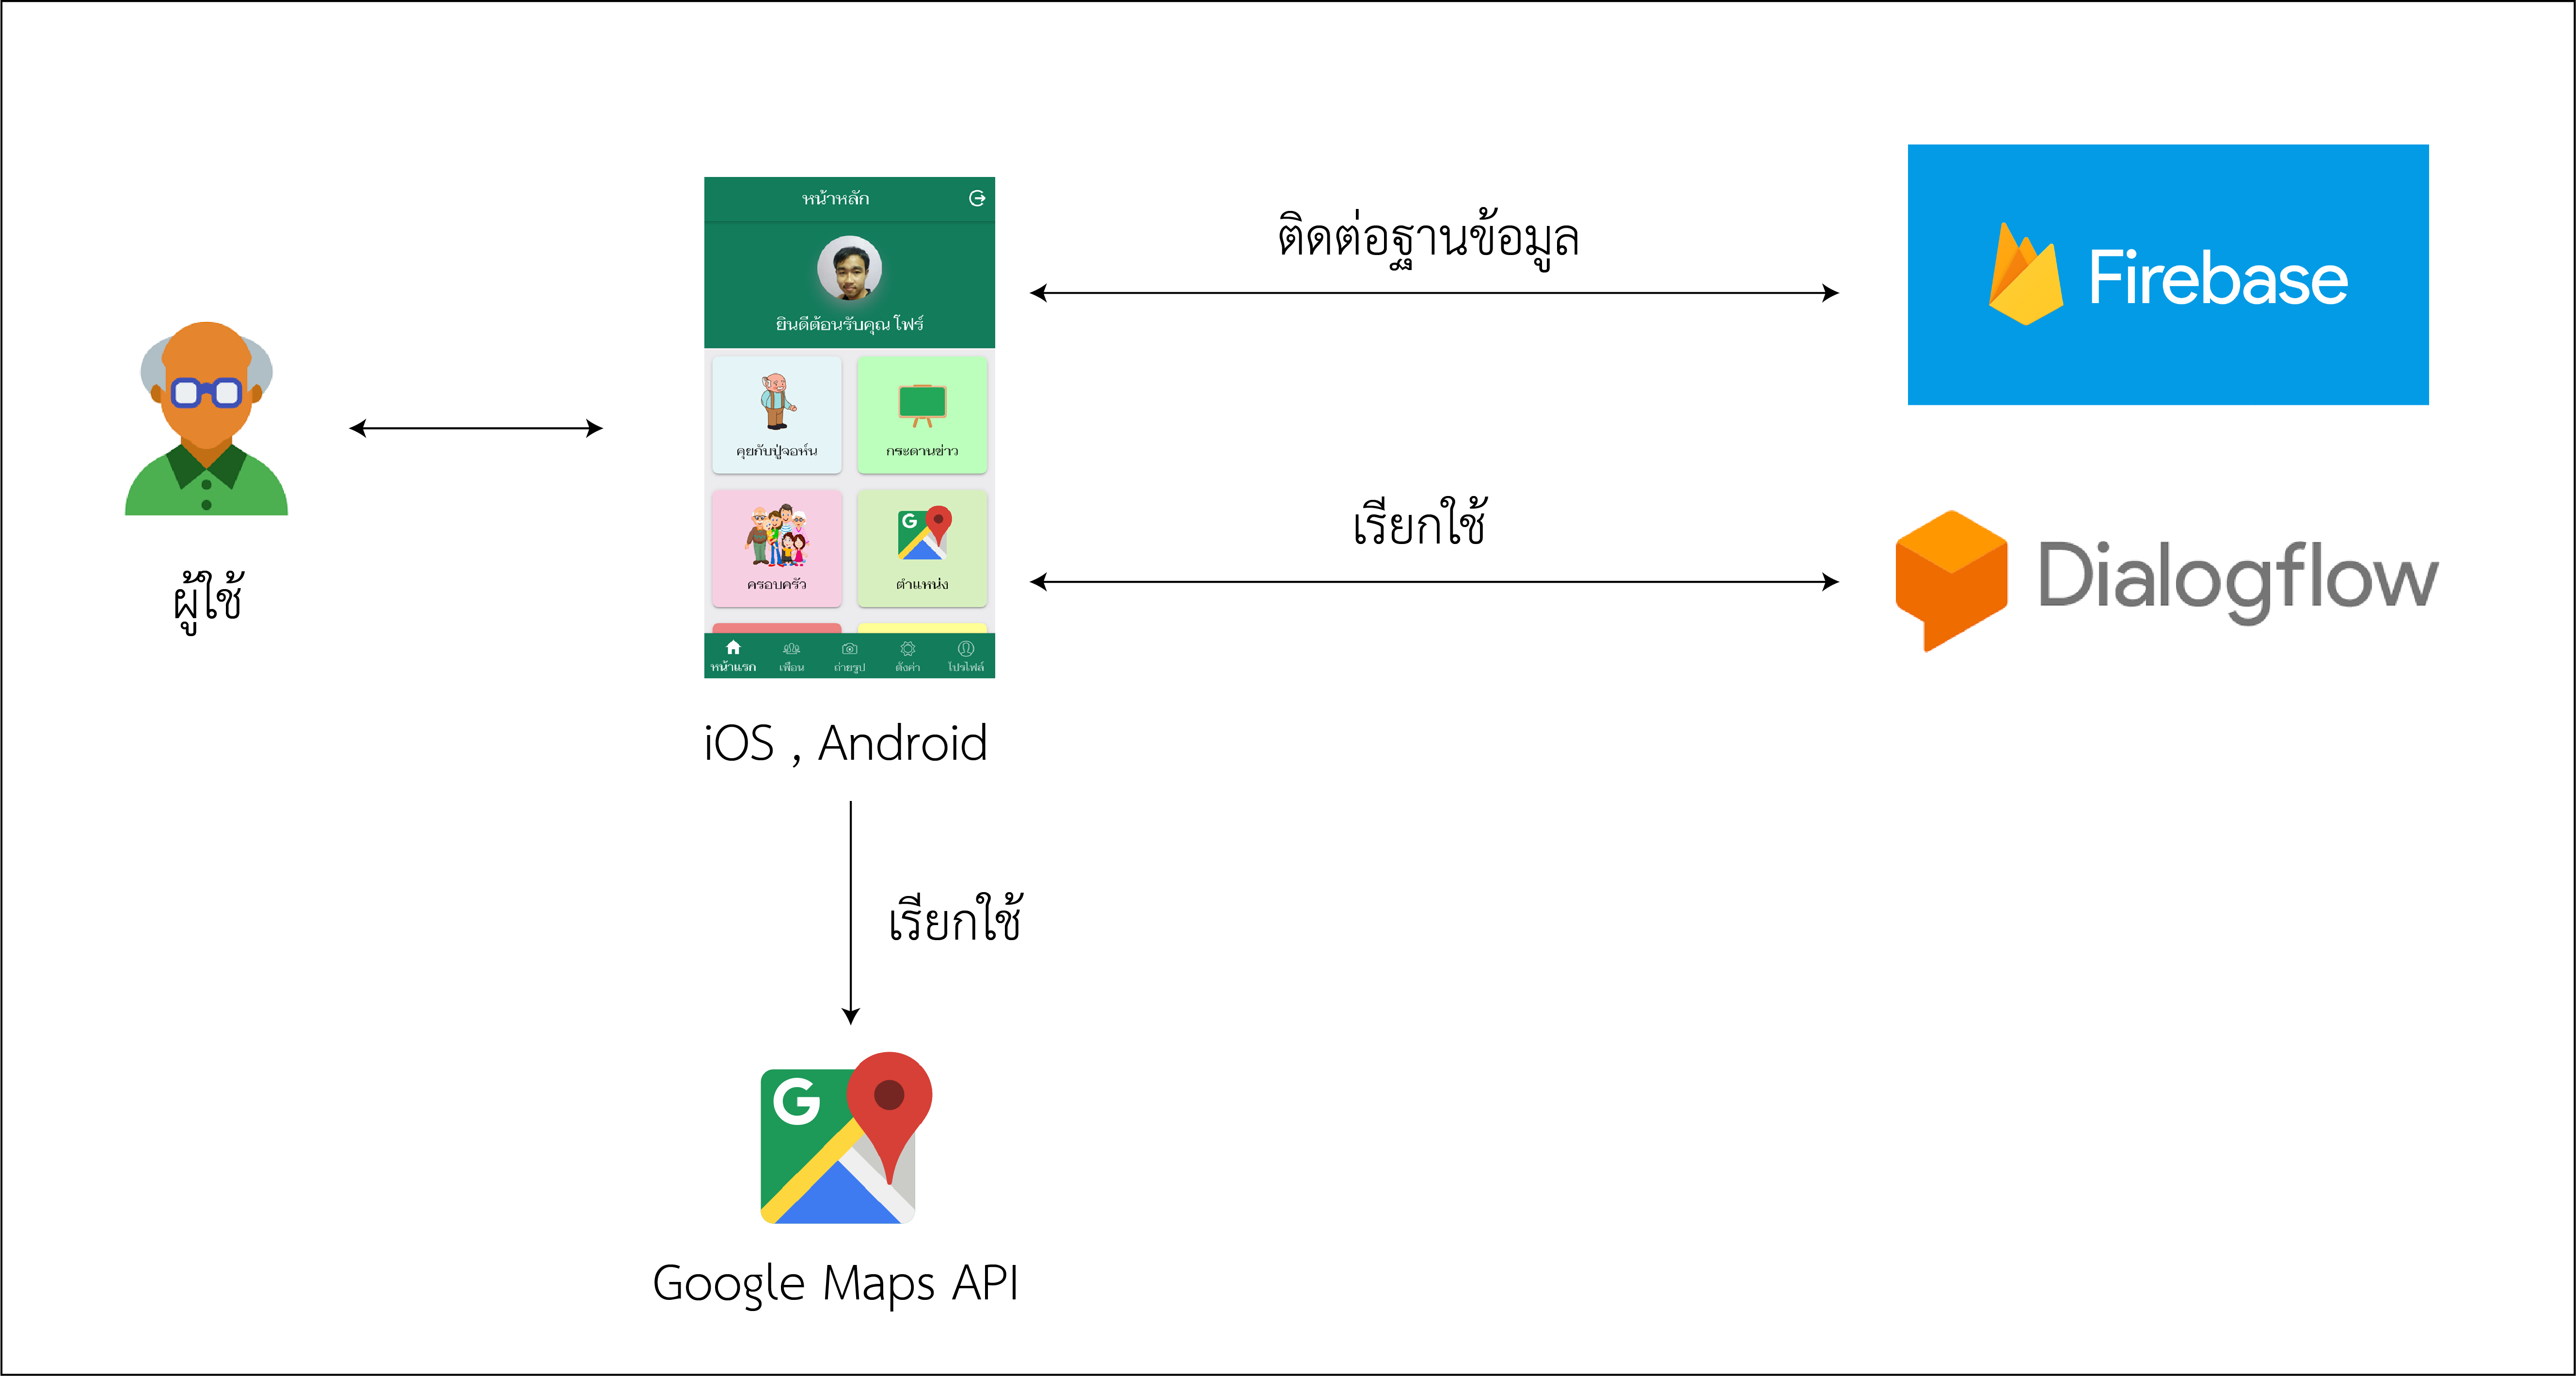
\includegraphics[width=\textwidth]{Figures/3/architecture/structure_app}
   		\caption{System architecture แอปพลิเคชันสูงวัยมายเฟรนด์}
   		\label{Fig:architecture}
   	\end{figure}
   
   จากรูปที่ \ref{Fig:architecture} สามารถอธิบายโครงสร้างและเทคโนโลยีของระบบโดยแบ่งเป็น 3 ส่วนหลัก ดังนี้
   \begin{enumerate}
   	\item Database
   	 ระบบใช้บริการฐานข้อมูลแบบ NoSQL ของไฟร์เบสชื่อ Cloud Firestore
	  \item Server
	   กระบวนการทำงานในส่วนของเซิฟเวอร์ (server) แบ่งเป็น 3 ส่วนได้แก่
	   \begin{itemize}
	   	\item Dialogflow เป็น Platform ไว้สำหรับจัดการการโต้ตอบอัตโนมัติหรือแชทบอท
	   	\item Google Maps Api เป็น Api ของ Google ไว้สำหรับเรียกใช้งาน Google Maps เพื่อใช้งานแผนที่
	   	\item ชุดบริการไฟร์เบส Api ใช้สำหรับการทำงานกับบริการต่าง ๆ ของไฟร์เบสบนแฟลตฟอร์มที่แตกต่างกัน เช่น Authentication ใช้สำหรับการจัดการข้อมูลผู้ใช้หรือไฟร์เบส Storage ที่ใช้สำหรับจัดเก็บไฟล์เอกสารและรูปภาพต่าง ๆ เป็นต้น
	   \end{itemize}
	   \item Client
	    App Moblie แอปพลิเคชันทำงานบนอุปกรณ์พกพาสามารถใช้ได้ทั้งแอนดรอยด์และไอโอเอส
   \end{enumerate}

%  สิ้นสุด ภาพรวมของระบบ

%  เริ่มต้น การวิเคราะห์ความต้องการของระบบ

\section{การวิเคราะห์ความต้องการของระบบ}
\subsection{ความต้องการหลักของระบบ (Functional Requirements)}
	แอปพลิเคชันสูงวัยมายเฟรนด์ แบ่งความสามารถของระบบดังนี้
	\begin{enumerate}
		\item ผู้ใช้งาน
			\begin{itemize}[label={--}]
				\item สามารถสมัครสมาชิกและเข้าสู่ระบบได้
				\item สามารถดู สร้าง แก้ไข ลบ โพสท์ได้
				\item สามารคุยโต้ตอบกับแชทบอทได้
				\item สามารถดูตำแหน่งของคนในครอบครัวได้
				\item สามารถส่งแจ้งเตือนรูปแบบการโทร หรือข้อความ ไปหาคนในครอบครัวได้
				\item สามารถเพิ่ม ลบ เพื่อนได้
				\item สามารถรับการแจ้งเตือนการทานยาได้
				\item สามารถดูและแก้ไขข้อมูลส่วนตัวได้
			\end{itemize}
	\end{enumerate}

\subsection{Non-functional Requirements}
\begin{enumerate}
		\item แอปพลิเคชัน
		\begin{itemize}[label={--}]
			\item แชทบอทสามารถตอบโต้ได้ตรงประเด็น
			\item มีความรวดเร็วในการกดไลท์
			\item สามารถใช้งานได้รวดเร็ว
			\item สามารถดูตำแหน่งของคนในครอบครัวแบบ Realtime
			\item สามารถแจ้งเตือนการทานยาได้เมื่อปิดแอปพลิเคชันอย่างสมบูรณ์
		\end{itemize}
	\end{enumerate}
%  สิ้นสุด การวิเคราะห์ความต้องการของระบบ
	
%  เริ่มต้น User Interface Design

\section{การออกแบบส่วนติดต่อผู้ใช้}
ในการออกแบบส่วนติดต่อผู้ใช้ของแอปพลิเคชันสูงวัยมายเฟรนด์ ประกอบด้วยส่วนต่าง ๆ ดังนี้
	\subsection{หน้าเข้าสู่ระบบ}
		\begin{figure}[H]
			\centering
			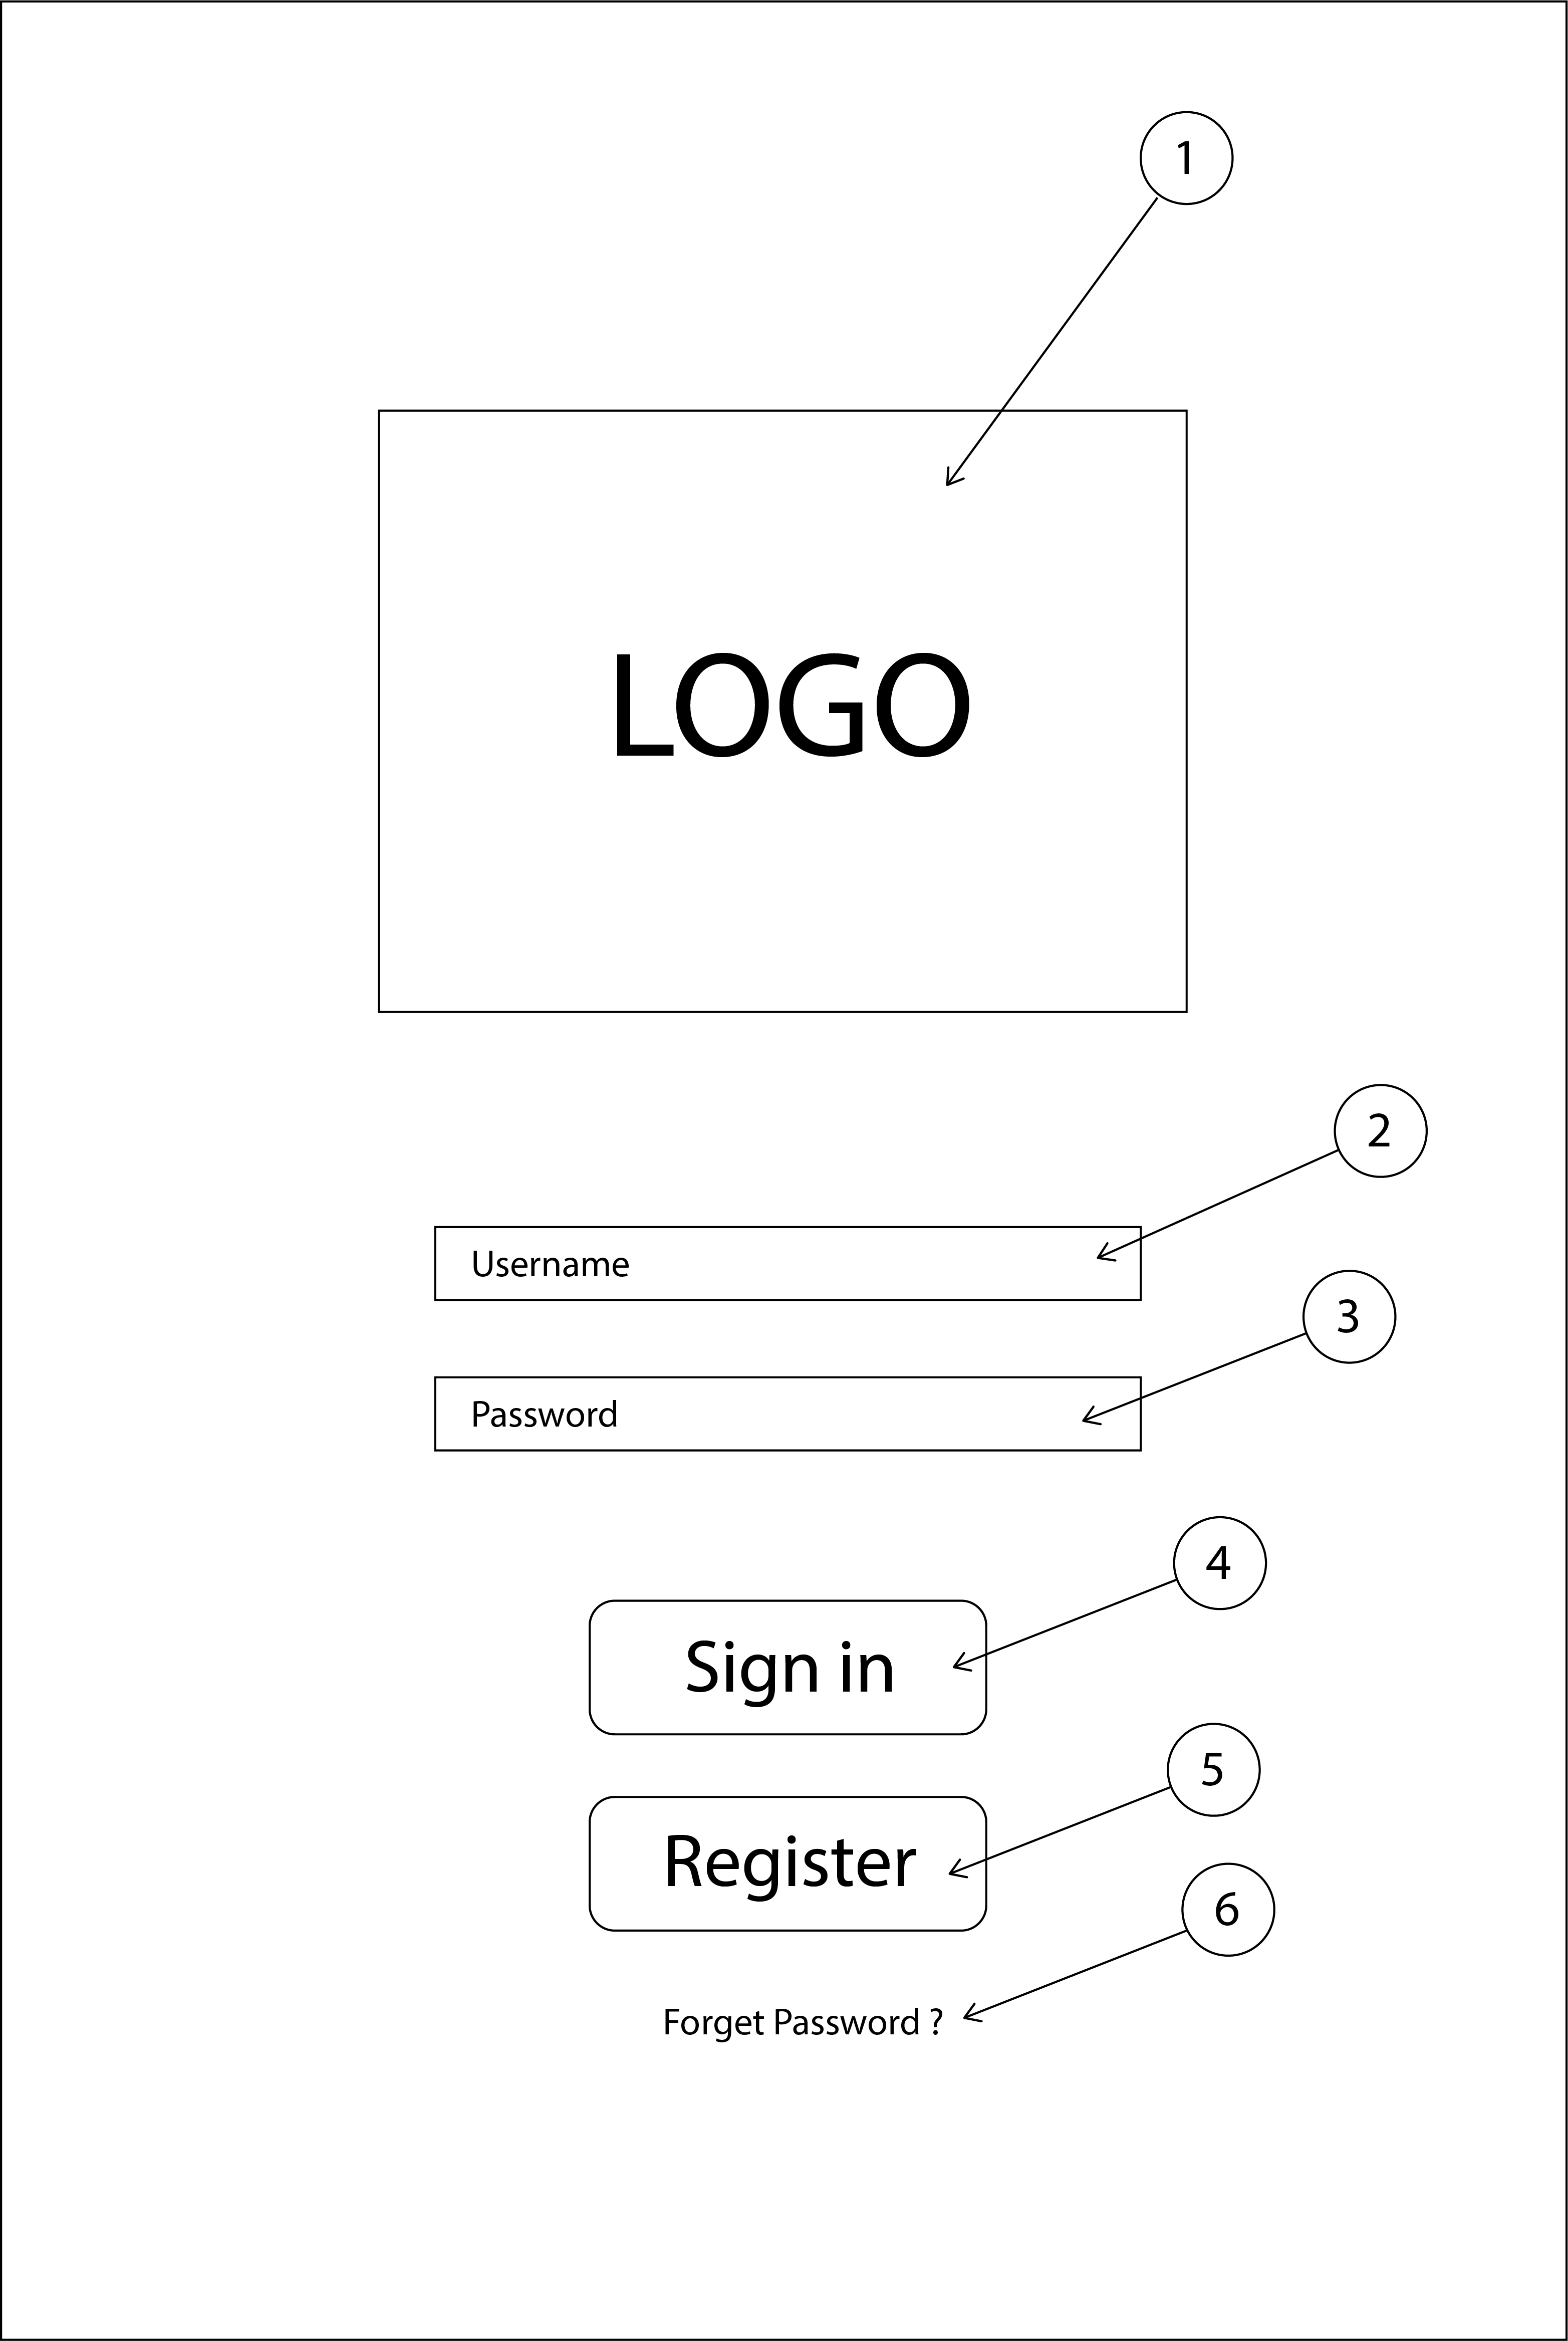
\includegraphics[width=0.6\textwidth]{Figures/3/UI/login}
			\caption{หน้าจอเข้าสู่ระบบ}
			\label{Fig:หน้าจอเข้าสู่ระบบ}
		\end{figure}
		จากภาพที่ \ref{Fig:หน้าจอเข้าสู่ระบบ} การออกแบบหน้าจอเข้าสู่ระบบประกอบไปด้วย 6 ส่วนดังนี้
		\begin{itemize}
			\item ส่วนที่ 1 โลโก้ของแอปพลิเคชัน
			\item ส่วนที่ 2 ช่องสำหรับกรอกชื่อผู้ใช้
			\item ส่วนที่ 3 ช่องสำหรับกรอกรหัสผ่าน
			\item ส่วนที่ 4 ปุ่มสำหรับเข้าสู่ระบบ
			\item ส่วนที่ 5 ปุ่มสำหรับสมัครสมาชิก
			\item ส่วนที่ 6 ข้อความสำหรับกดเมื่อลืมรหัสผ่าน
		\end{itemize}

		\begin{figure}[H]
			\centering
			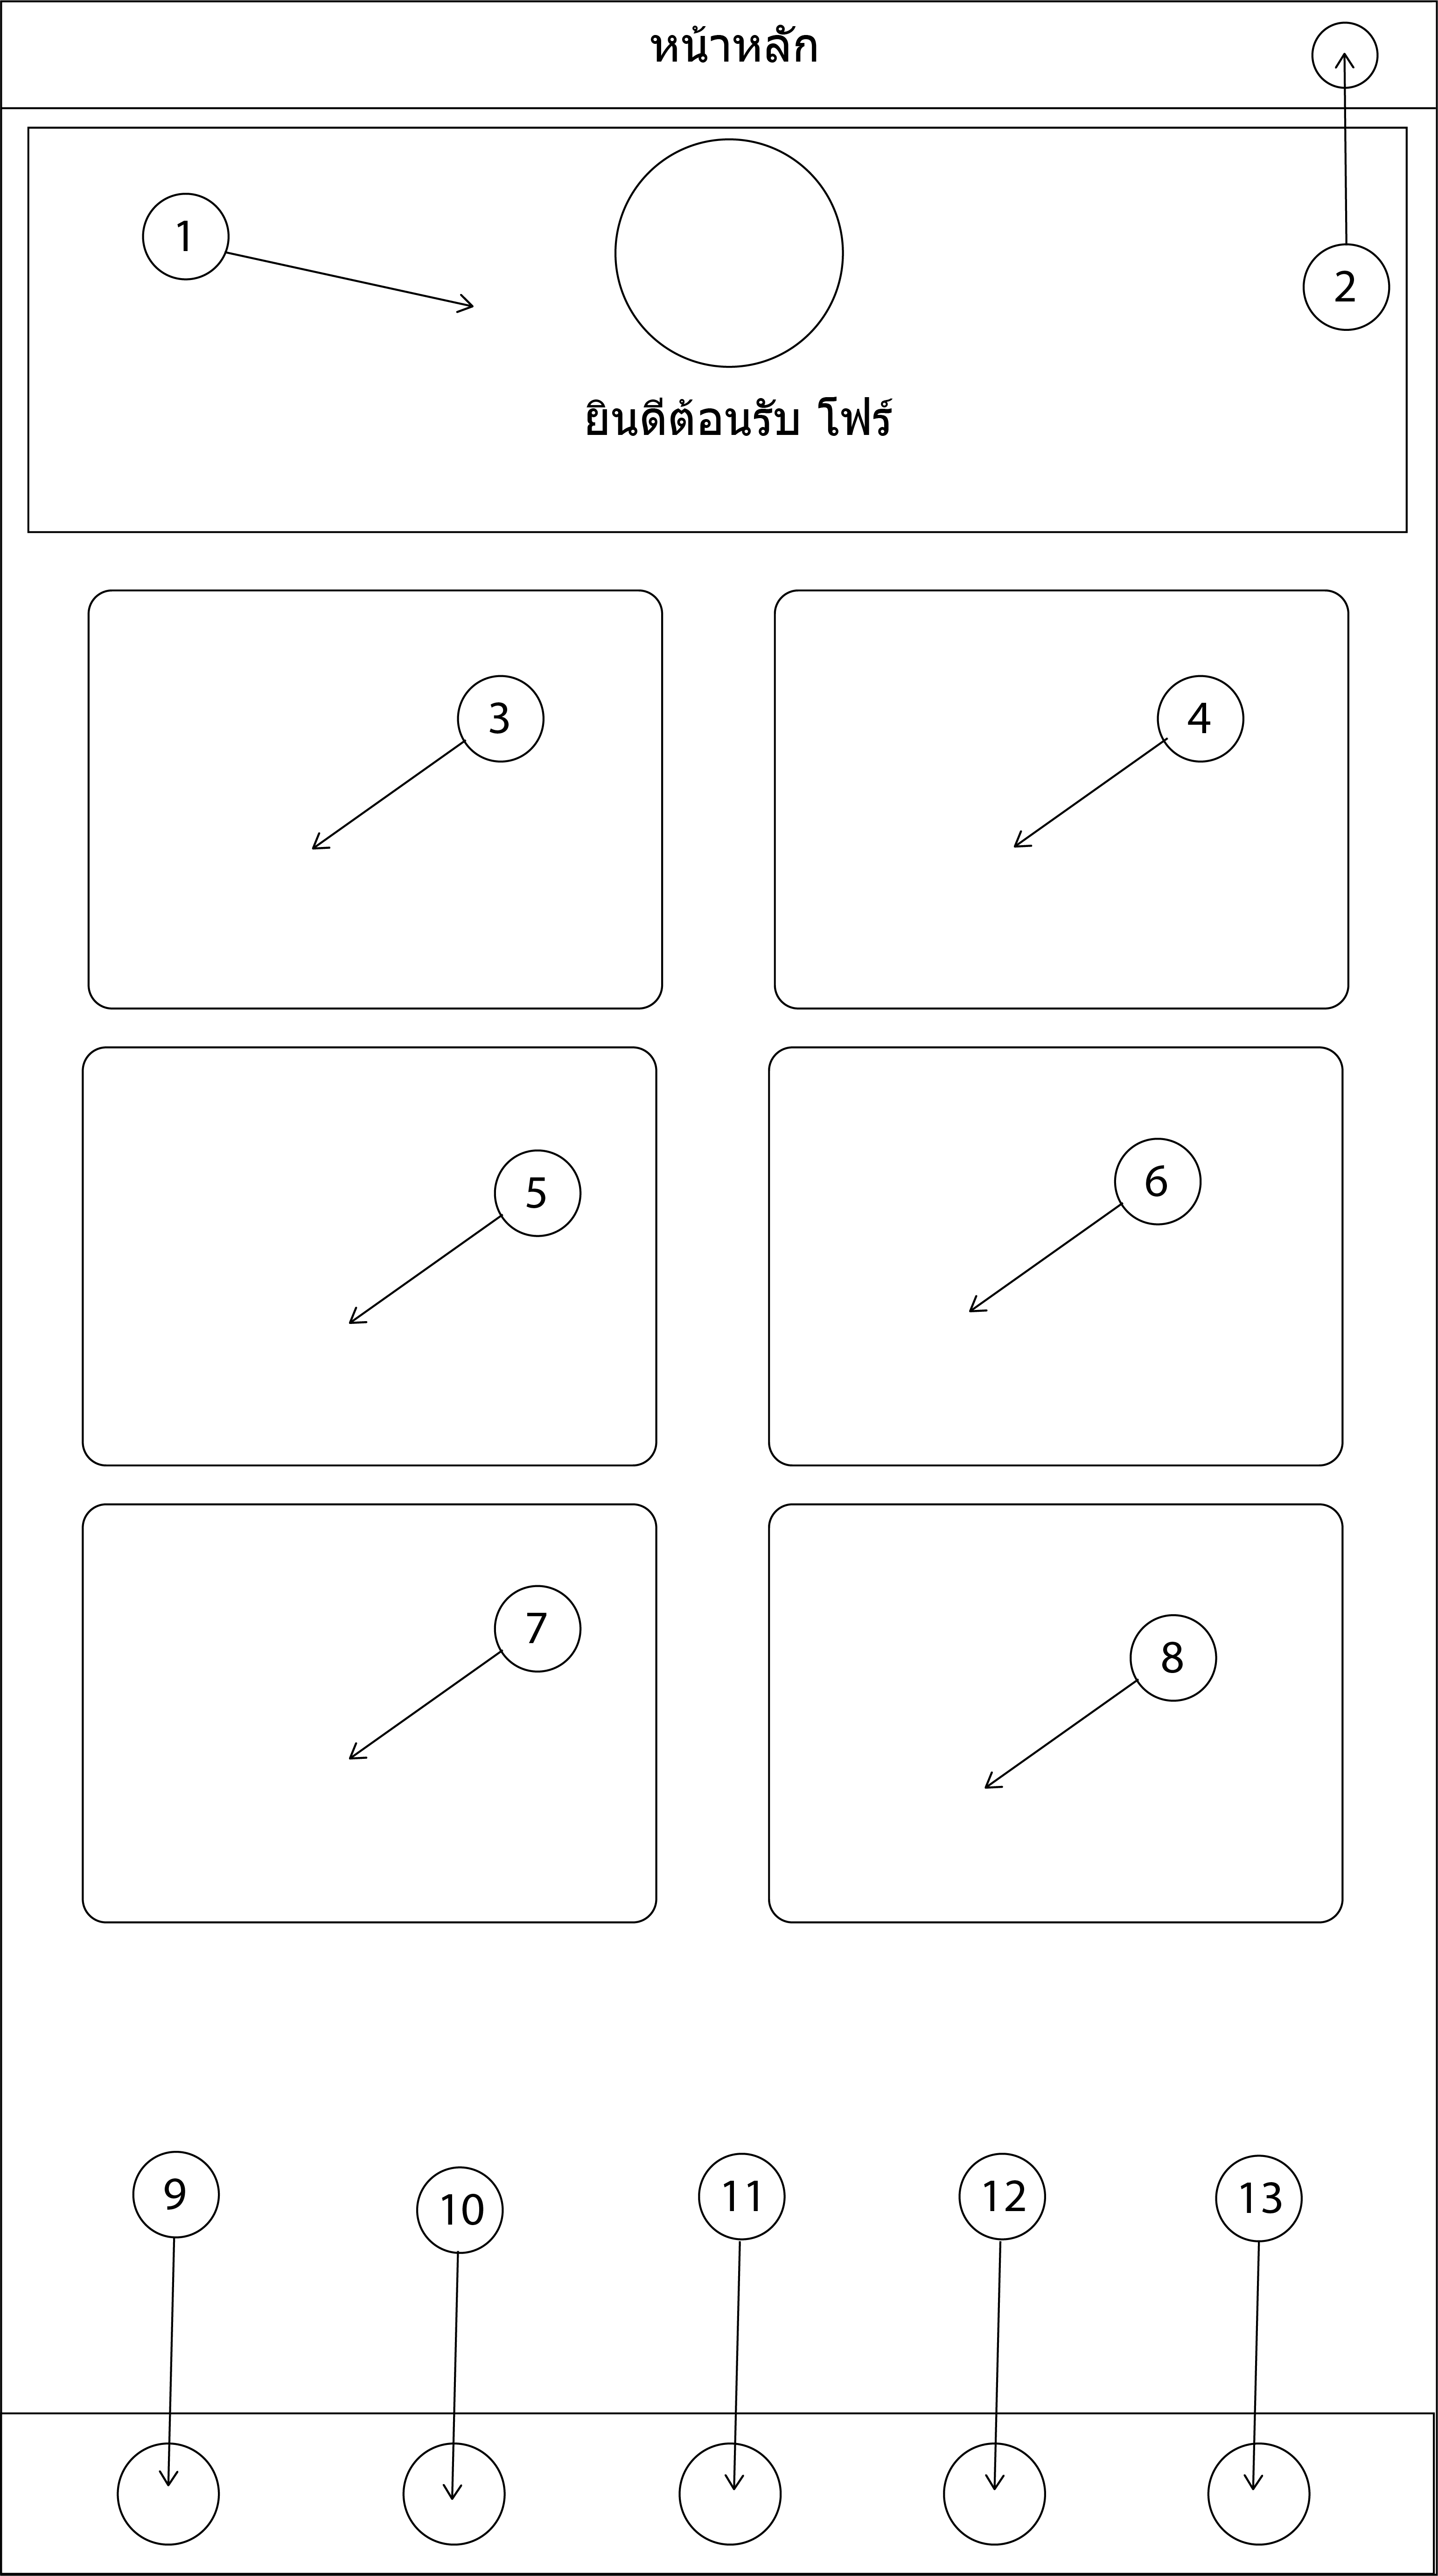
\includegraphics[width=0.6\textwidth]{Figures/3/UI/main}
			\caption{หน้าจอหลัก}
			\label{Fig:หน้าจอหลัก}
		\end{figure}
		จากภาพที่ \ref{Fig:หน้าจอหลัก} การออกแบบหลักประกอบไปด้วย 13 ส่วนดังนี้
		\begin{itemize}
			\item ส่วนที่ 1 ข้อมูลของผู้ใช้ประกอบไปด้วยรูปประจำตัวและชื่อผู้ใช้
			\item ส่วนที่ 2 ปุ่มสำหรับออกจากระบบ
			\item ส่วนที่ 3 ปุ่มสำหรับไปยังหน้าปู่จอห์นที่เป็นแชทบอท
			\item ส่วนที่ 4 ปุ่มสำหรับไปยังหน้ากระดานข่าว
			\item ส่วนที่ 5 ปุ่มสำหรับไปยังหน้าครอบครัว
			\item ส่วนที่ 6 ปุ่มสำหรับไปยังหน้าตำแหน่งของครอบครัว
			\item ส่วนที่ 7 ปุ่มสำหรับไปยังหน้าฉุกเฉิน
			\item ส่วนที่ 8 ปุ่มไปยังหน้าวิธีใช้งาน
			\item ส่วนที่ 9 ปุ่มไปยังหน้าหลักเราจะอยู่หน้านี้ทุกครั้งเมื่อเราเข้าสู่แอปพลิเคชัน
			\item ส่วนที่ 10 ปุ่มสำหรับไปยังหน้าเพื่อนและครอบครัว
			\item ส่วนที่ 11 ปุ่มเพื่อโพสท์ข้อความหรือรูปภาพ
			\item ส่วนที่ 12 ปุ่มสำหรับไปหน้าตั้งค่า
			\item ส่วนที่ 13 ปุ่มสำหรับไปยังหน้าโปรไฟล์หรือข้อมูลส่วนตัว
		\end{itemize}

		\begin{figure}[H]
			\centering
			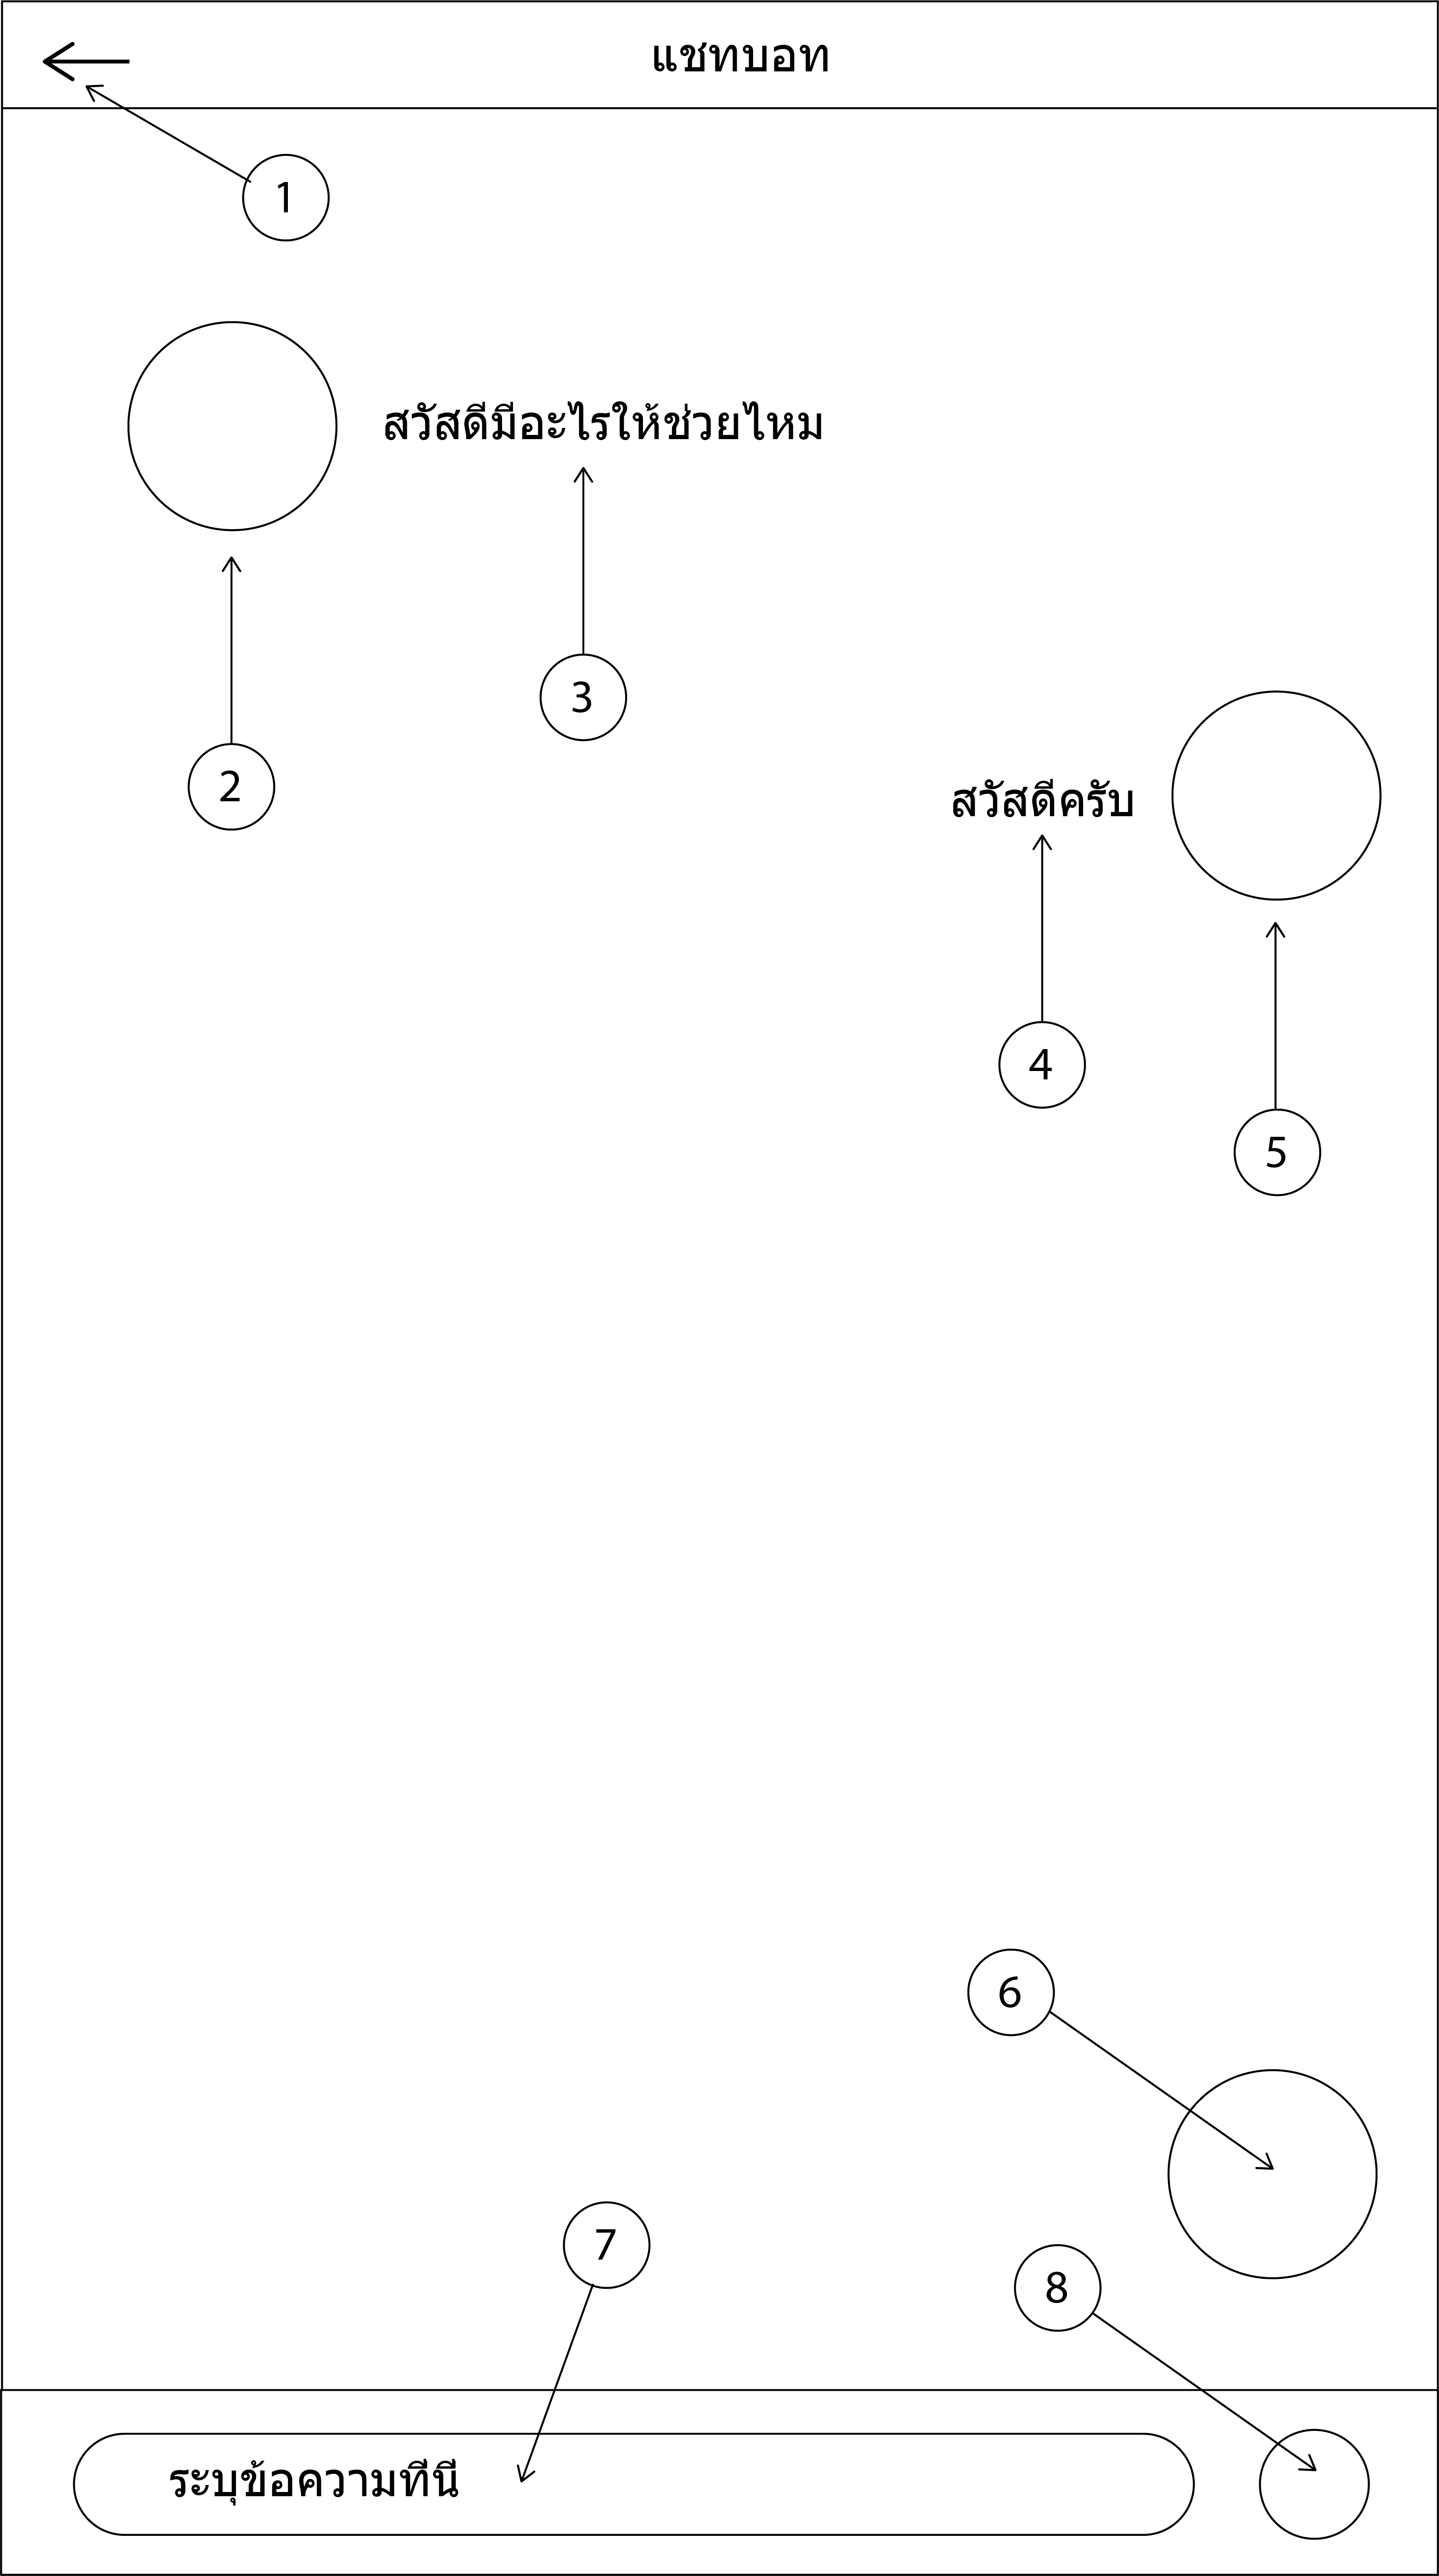
\includegraphics[width=0.6\textwidth]{Figures/3/UI/chatbot}
			\caption{หน้าแชทบอทคุยกับปู่จอห์น}
			\label{Fig:แชทบอท}
		\end{figure}
		จากภาพที่ \ref{Fig:แชทบอท} การออกแบบหลักประกอบไปด้วย 8 ส่วนดังนี้
		\begin{itemize}
			\item ส่วนที่ 1 ปุ่มลูกศรกลับไปยังหน้าจอหลัก
			\item ส่วนที่ 2 รูปประจำตัวของปู่จอห์น
			\item ส่วนที่ 3 ข้อความที่ปู่จอห์นตอบกลับผู้ใช้
			\item ส่วนที่ 4 ข้อความของผู้ใช้
			\item ส่วนที่ 5 รูปประจำตัวของผู้ใช้
			\item ส่วนที่ 6 ปุ่มสำหรับพิมพ์ข้อความด้วยเสียง (Speech to text)
			\item ส่วนที่ 7 ช่องสำหรับกรอกข้อความที่จะแสดงในส่วนที่ 4
			\item ส่วนที่ 8 ปุ่มสำหรับยืนยันข้อความส่วนที่ 7
		\end{itemize}

		\begin{figure}[H]
			\centering
			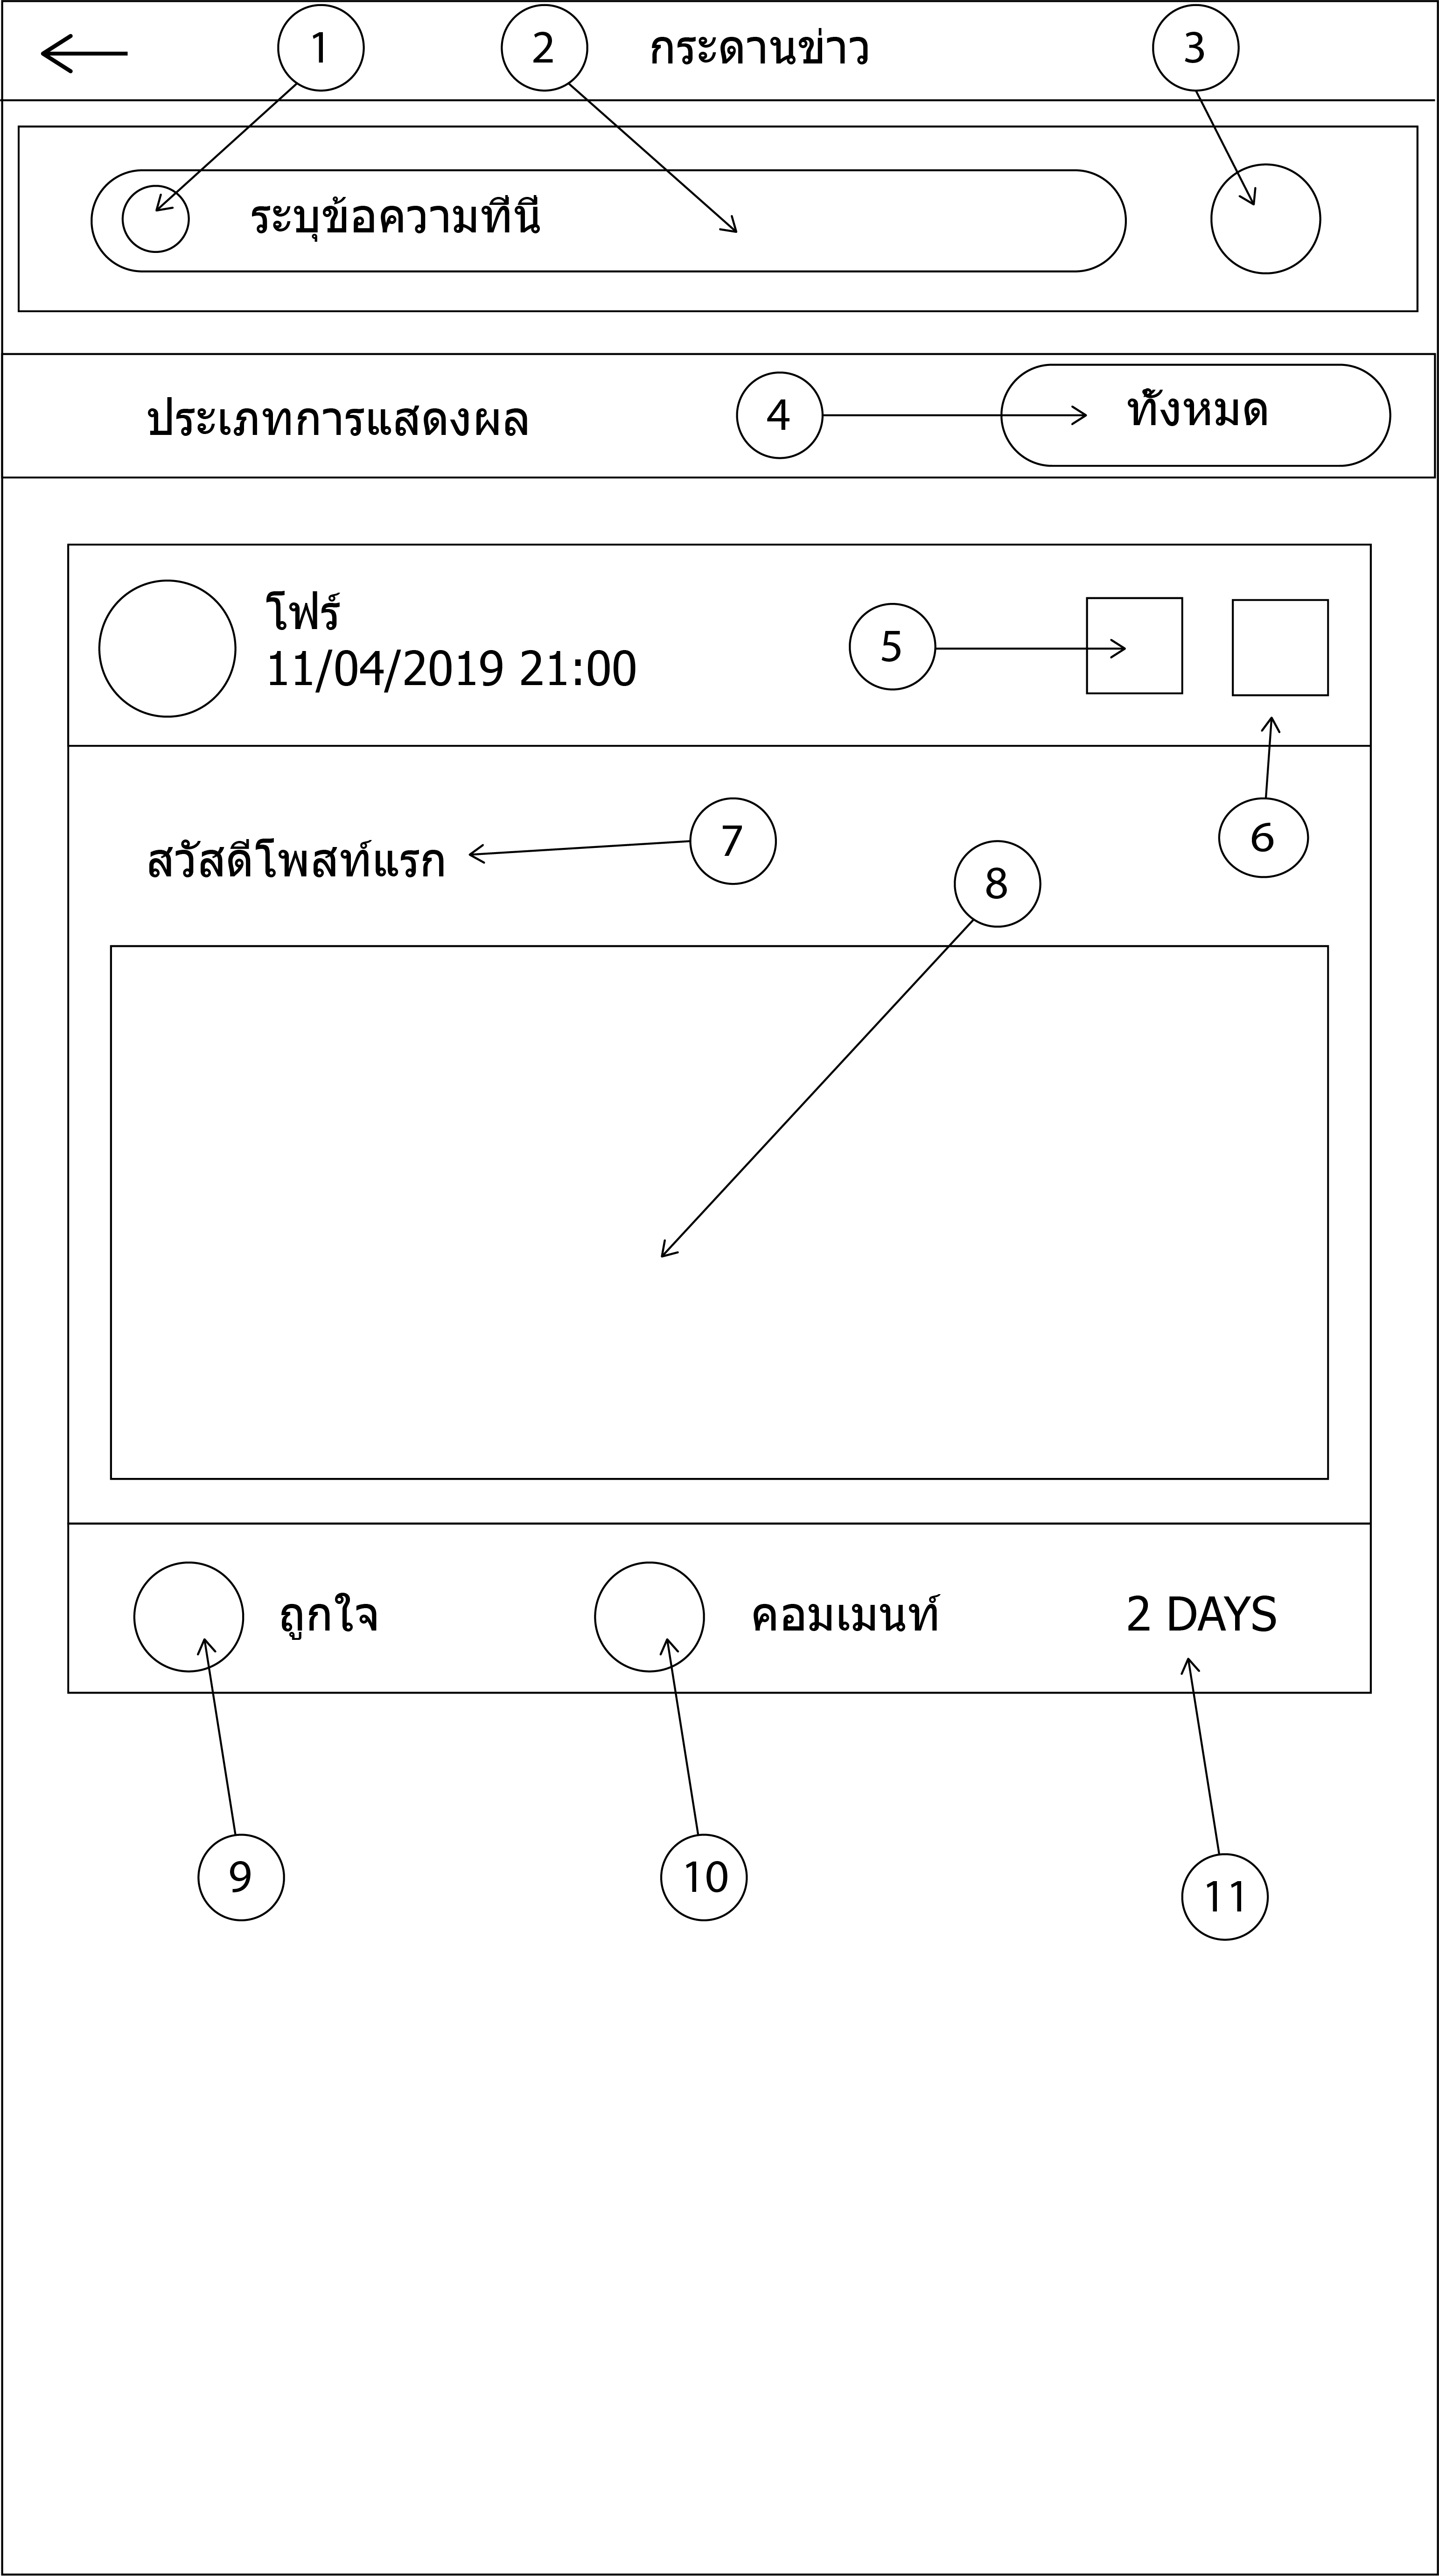
\includegraphics[width=0.6\textwidth]{Figures/3/UI/board}
			\caption{หน้าจอกระดานข่าว}
			\label{Fig:กระดานข่าว}
		\end{figure}
		จากภาพที่ \ref{Fig:กระดานข่าว} การออกแบบหลักประกอบไปด้วย 11 ส่วนดังนี้
		\begin{itemize}
			\item ส่วนที่ 1 ปุ่มสำหรับเพิ่มรูปภาพสำหรับโพสท์มีสองส่วนคือ ถ่ายรูปและเลือกรูปจากแกลอรี่
			\item ส่วนที่ 2 ช่องสำหรับกรอกข้อความที่จะโพสท์
			\item ส่วนที่ 3 ปุ่มสำหรับยืนยันการโพสท์หลังจากคลิกจะมีการเลือกประเภทได้ 3 แบบคือ กีฬา, ศาสนา, ดนตรี
			\item ส่วนที่ 4 ลิสท์สำหรับเลือกแสดงเฉพาะประเภทที่ต้องการมี 4 แบบได้แก่ ทั้งหมด, กีฬา, ศาสนา, ดนตรี
			\item ส่วนที่ 5 ปุ่มสำหรับแก้ไขโพสท์
			\item ส่วนที่ 6 ปุ่มสำหรับลบโพสท์
			\item ส่วนที่ 7 ข้อความโพสท์ของผู้ใช้
			\item ส่วนที่ 8 รูปภาพโพสท์ของผู้ใช้
			\item ส่วนที่ 9 ปุ่มสำหรับกดถูกใจ
			\item ส่วนที่ 10 ปุ่มสำหรับแสดงความคิดเห็น
			\item ส่วนที่ 11 ข้อความแสดงระยะเวลาหลังจากโพสท์ถูกสร้าง
		\end{itemize}

		\begin{figure}[H]
			\centering
			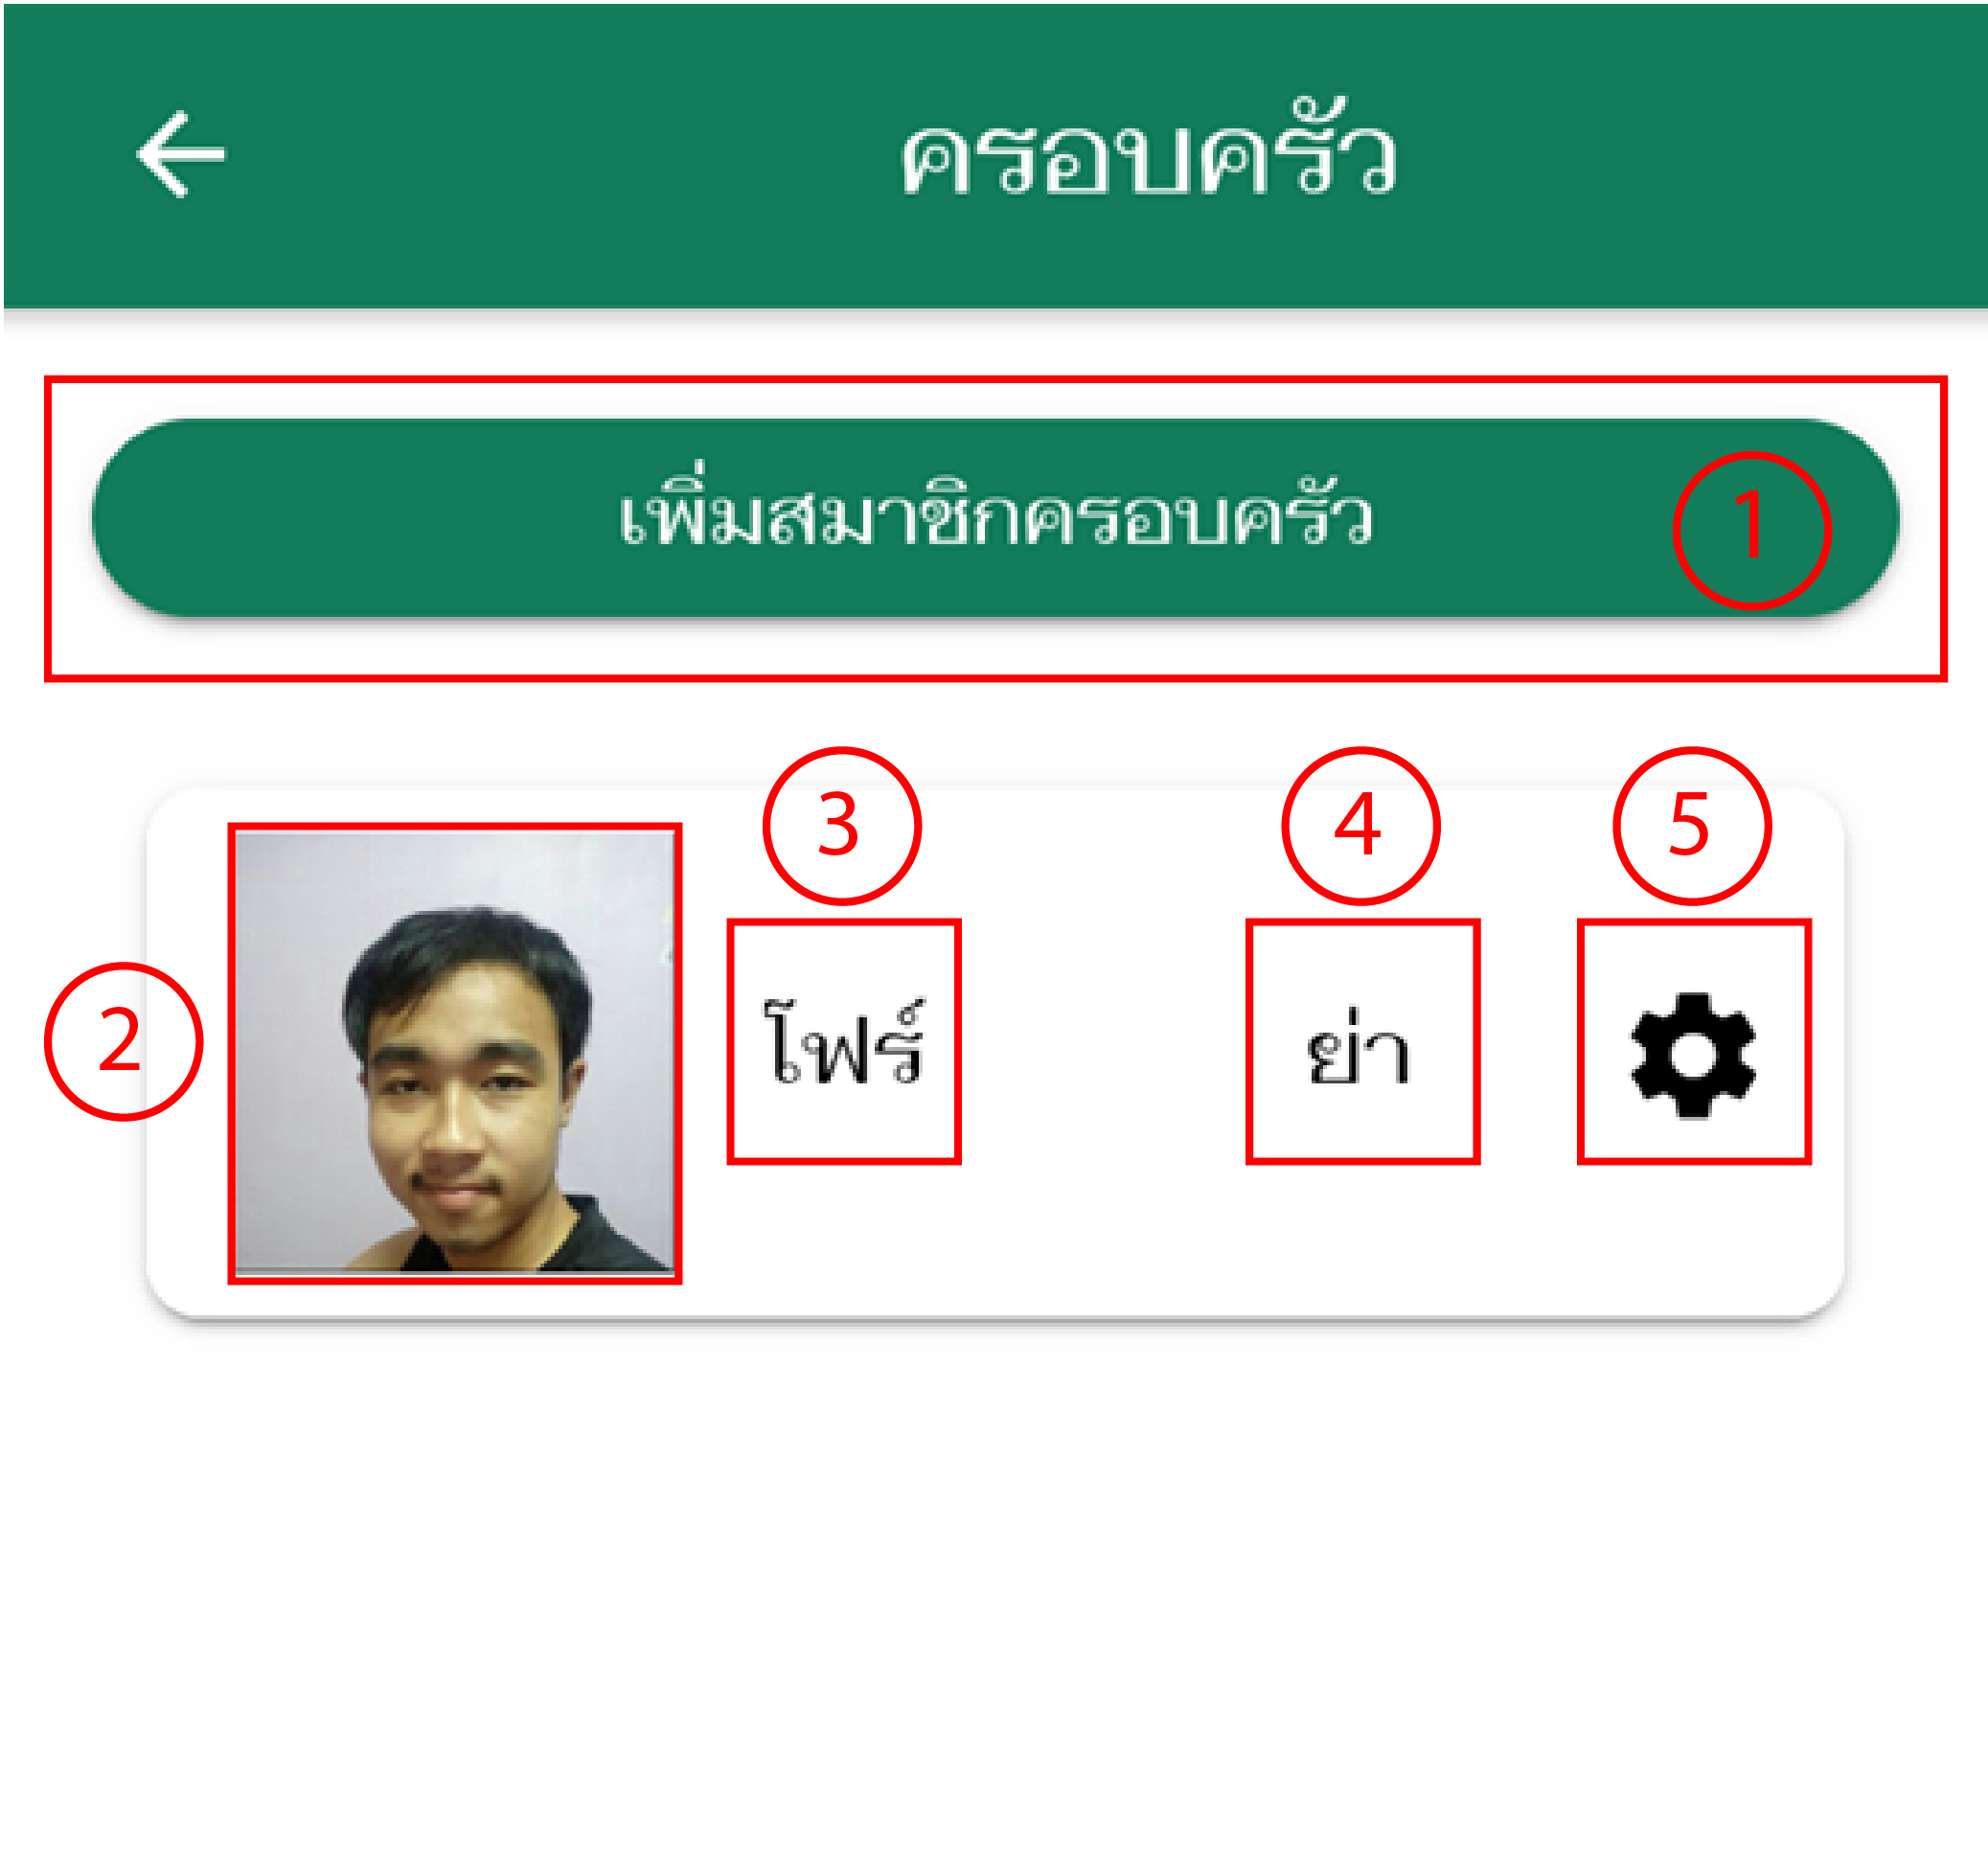
\includegraphics[width=0.6\textwidth]{Figures/3/UI/family}
			\caption{หน้าครอบครัว}
			\label{Fig:ครอบครัว}
		\end{figure}
		จากภาพที่ \ref{Fig:ครอบครัว} การออกแบบหลักประกอบไปด้วย 5 ส่วนดังนี้
		\begin{itemize}
			\item ส่วนที่ 1 ปุ่มสำหรับเพิ่มสมาชิกในครอบครัว
			\item ส่วนที่ 2 รูปภาพของสมาชิกในครอบครัว
			\item ส่วนที่ 3 ชื่อของสมาชิกในครอบครัว
			\item ส่วนที่ 4 สถานะของครอบครัว
			\item ส่วนที่ 5 ปุ่มสำหรับจัดการสมาชิกครอบครัวได้แก่ แก้ไขสถานะ ลบสมาชิก
		\end{itemize}

		\begin{figure}[H]
			\centering
			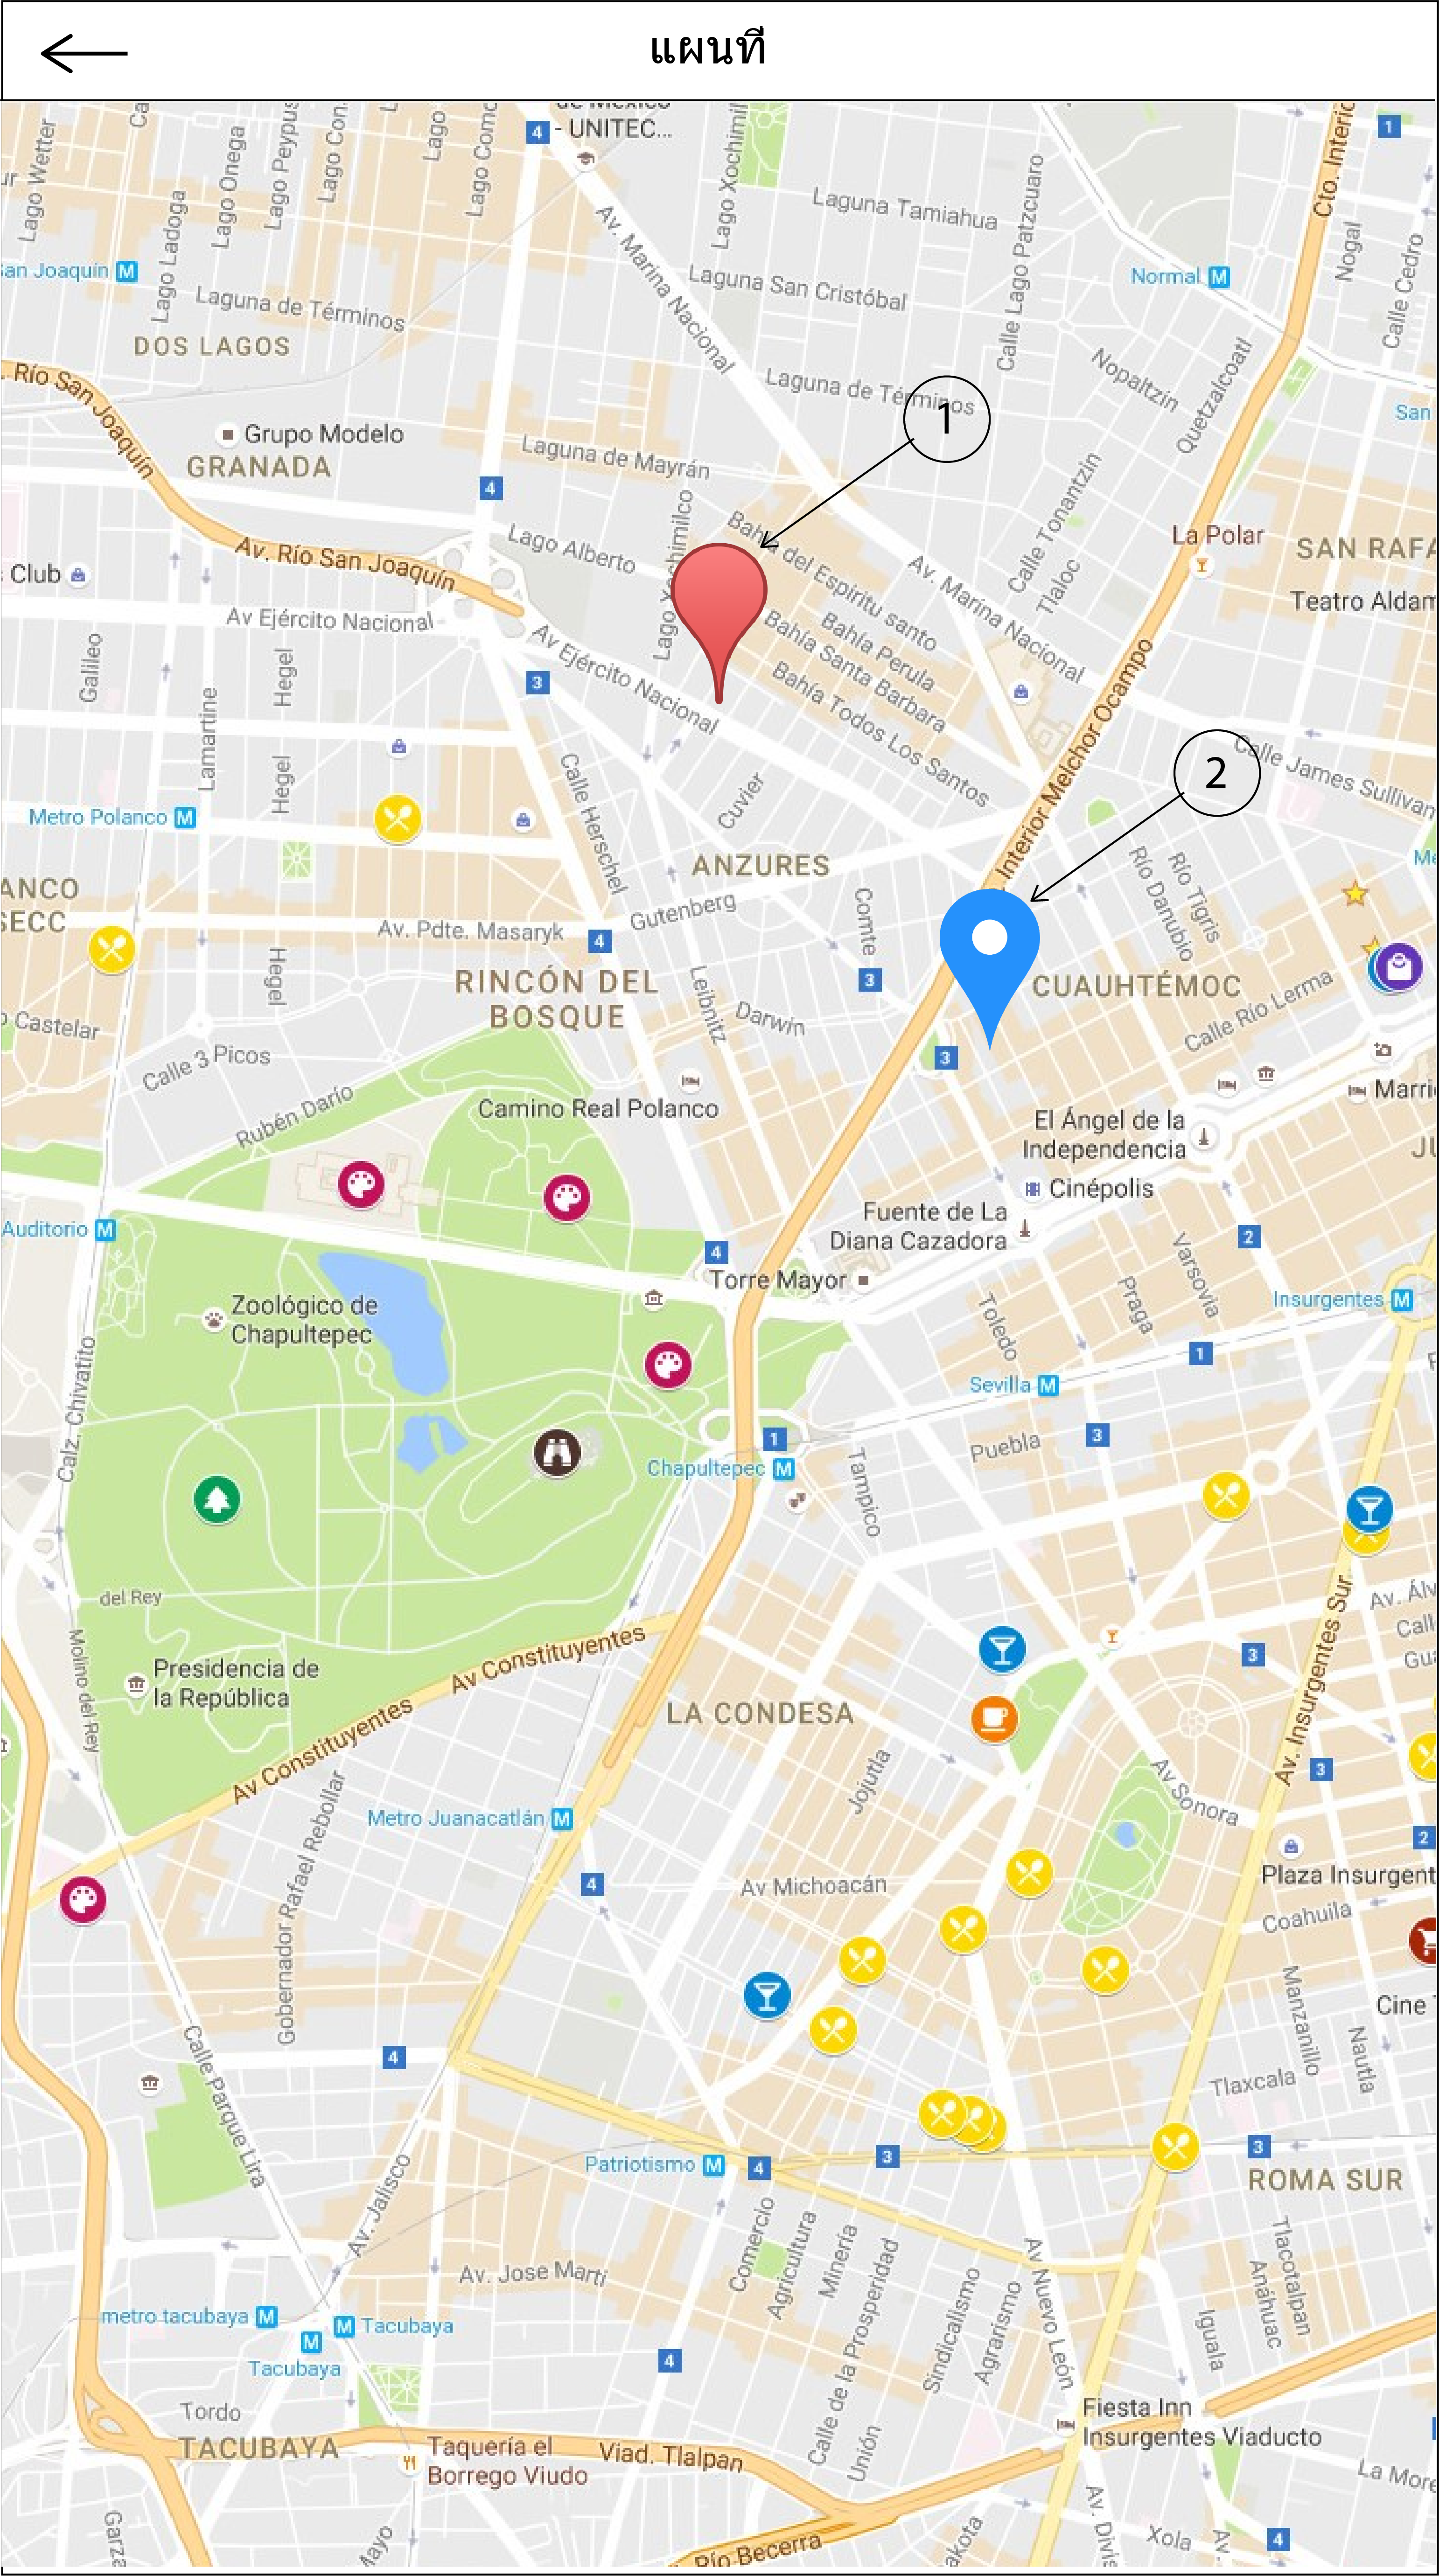
\includegraphics[width=0.6\textwidth]{Figures/3/UI/maps}
			\caption{หน้าแสดงตำแหน่งของครอบครัว}
			\label{Fig:แผนที่}
		\end{figure}
		จากภาพที่ \ref{Fig:แผนที่} การออกแบบหลักประกอบไปด้วย 2 ส่วนดังนี้
		\begin{itemize}
			\item ส่วนที่ 1 แสดงตำแหน่งของผู้ใช้
			\item ส่วนที่ 2 แสดงตำแหน่งของสมาชิกในครอบครัว
		\end{itemize}

		\begin{figure}[H]
			\centering
			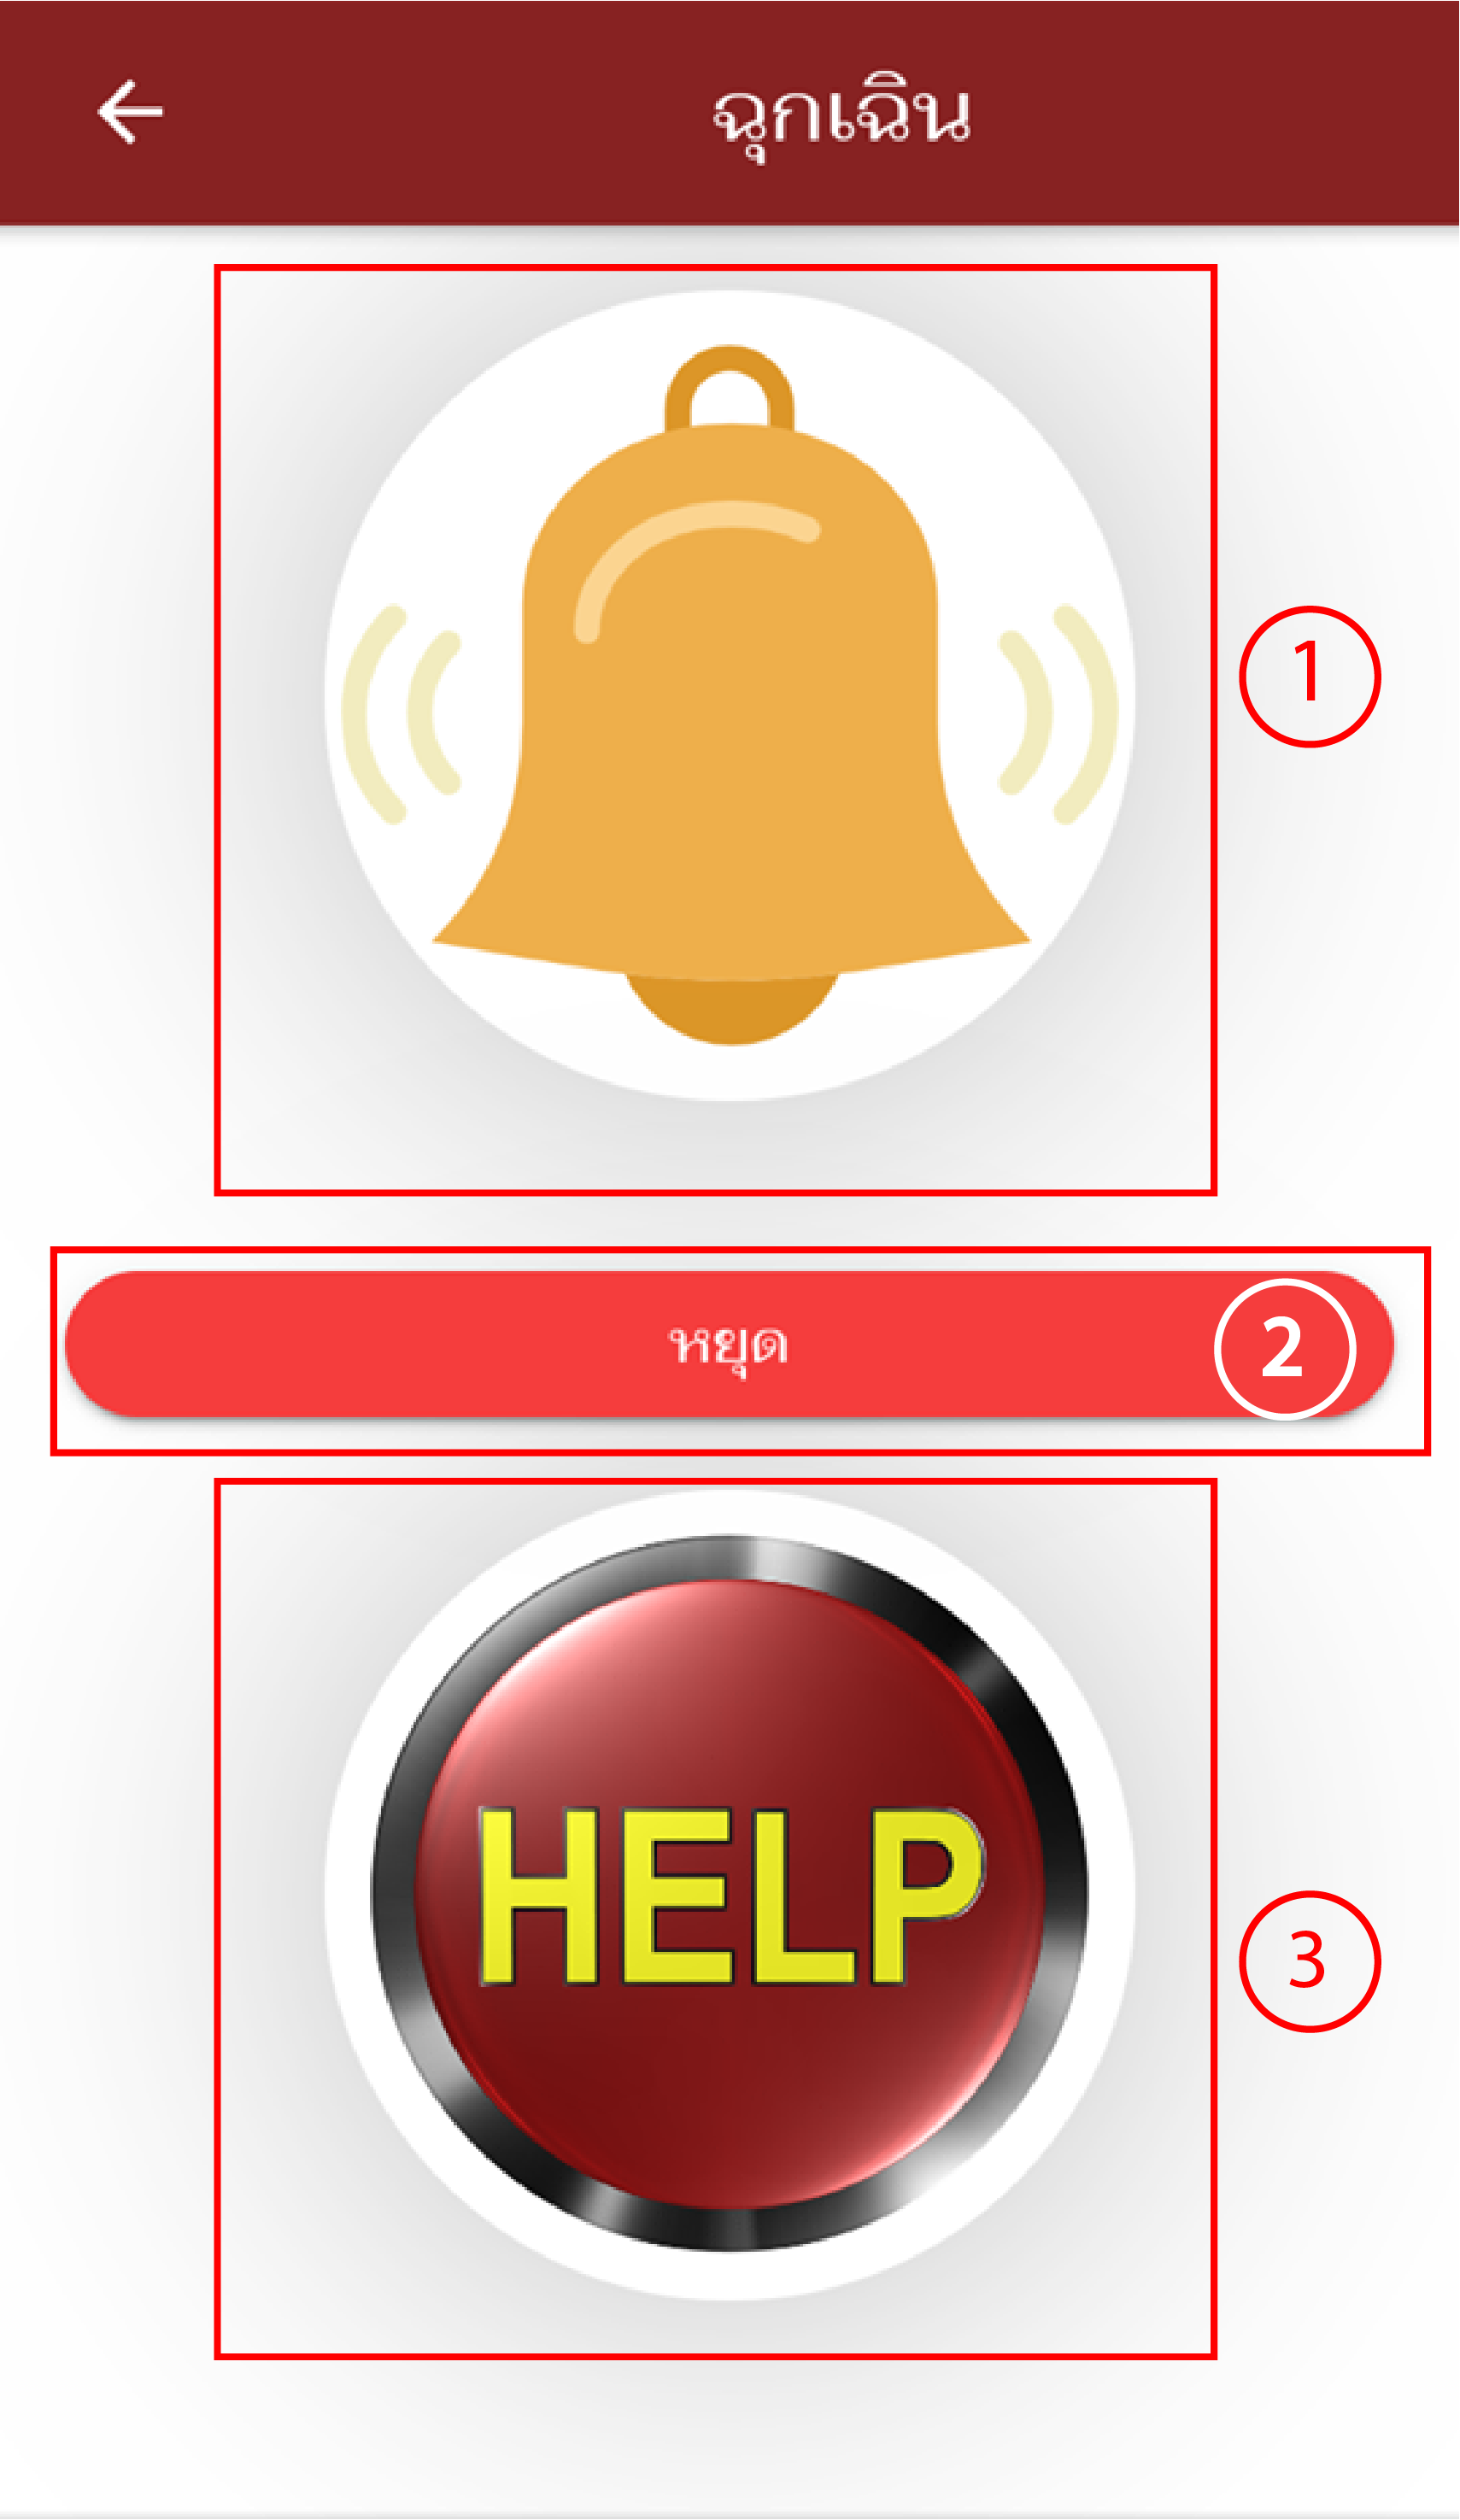
\includegraphics[width=0.6\textwidth]{Figures/3/UI/help}
			\caption{หน้าฉุกเฉิน}
			\label{Fig:ฉุกเฉิน}
		\end{figure}
		จากภาพที่ \ref{Fig:ฉุกเฉิน} การออกแบบหลักประกอบไปด้วย 2 ส่วนดังนี้
		\begin{itemize}
			\item ส่วนที่ 1 ปุ่มสำหรับแสดงเสียงเพื่อขอความช่วยเหลือ
			\item ส่วนที่ 2 ปุ่มสำหรับไปยังหน้าเลือกครอบครัวเพื่อขอความช่วยเหลือจากครอบครัว
		\end{itemize}

		\begin{figure}[H]
			\centering
			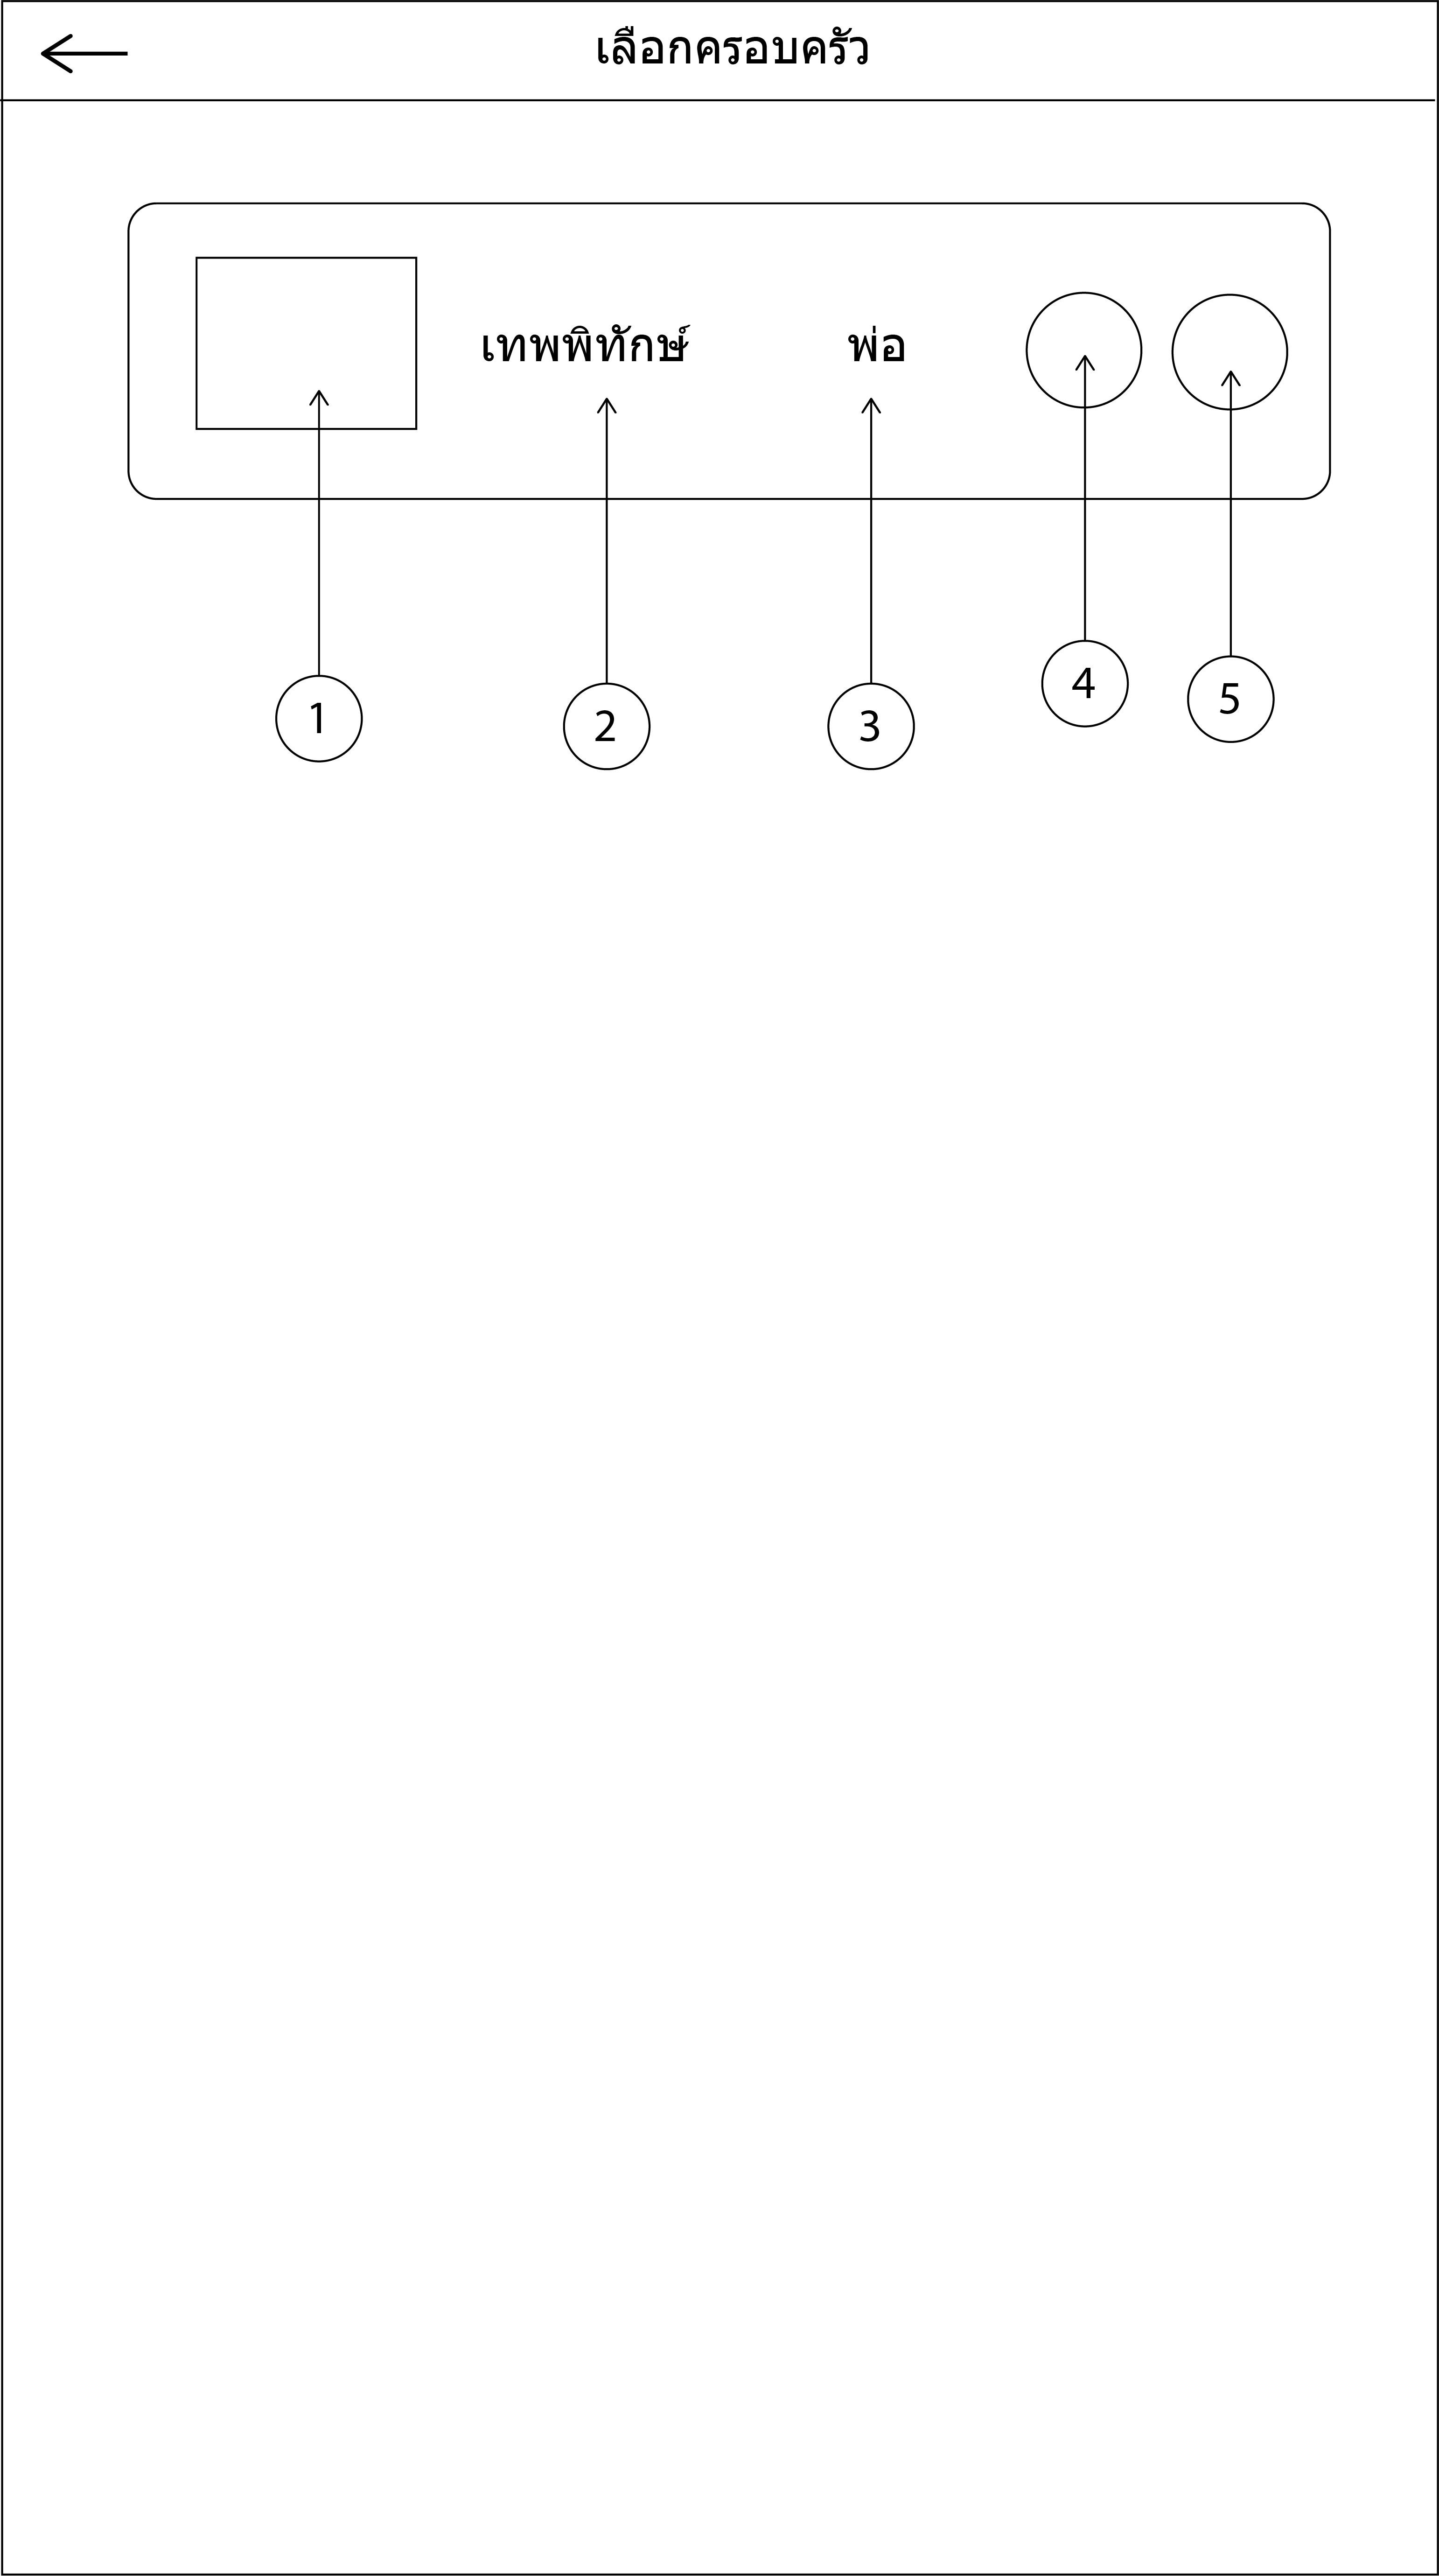
\includegraphics[width=0.6\textwidth]{Figures/3/UI/helpfamily}
			\caption{หน้าเลือกครอบครัว}
			\label{Fig:เลือกครอบครัว}
		\end{figure}
		จากภาพที่ \ref{Fig:เลือกครอบครัว} การออกแบบหลักประกอบไปด้วย 5 ส่วนดังนี้
		\begin{itemize}
			\item ส่วนที่ 1 รูปประจำตัวของสมาชิกในครอบครัว
			\item ส่วนที่ 2 ชื่อของสมาชิกในครอบครัว
			\item ส่วนที่ 3 สถานะของครอบครัว
			\item ส่วนที่ 4 ปุ่มสำหรับโทรไปยังหมายเลขของสมาชิกในครอบครัว
			\item ส่วนที่ 5 ปุ่มสำหรับส่งข้อความไปยังสมาชิกในครอบครัวมีข้อความดังนี้ "ช่วยด้วย !!! นี่ [ชื่อผู้ใช้] เอง ตอนนี้มีปัญหาช่วยติดต่อกลับมาที่ [เบอร์ผู้ใช้] ด้วยนะ ด่วนๆ"
		\end{itemize}

		\begin{figure}[H]
			\centering
			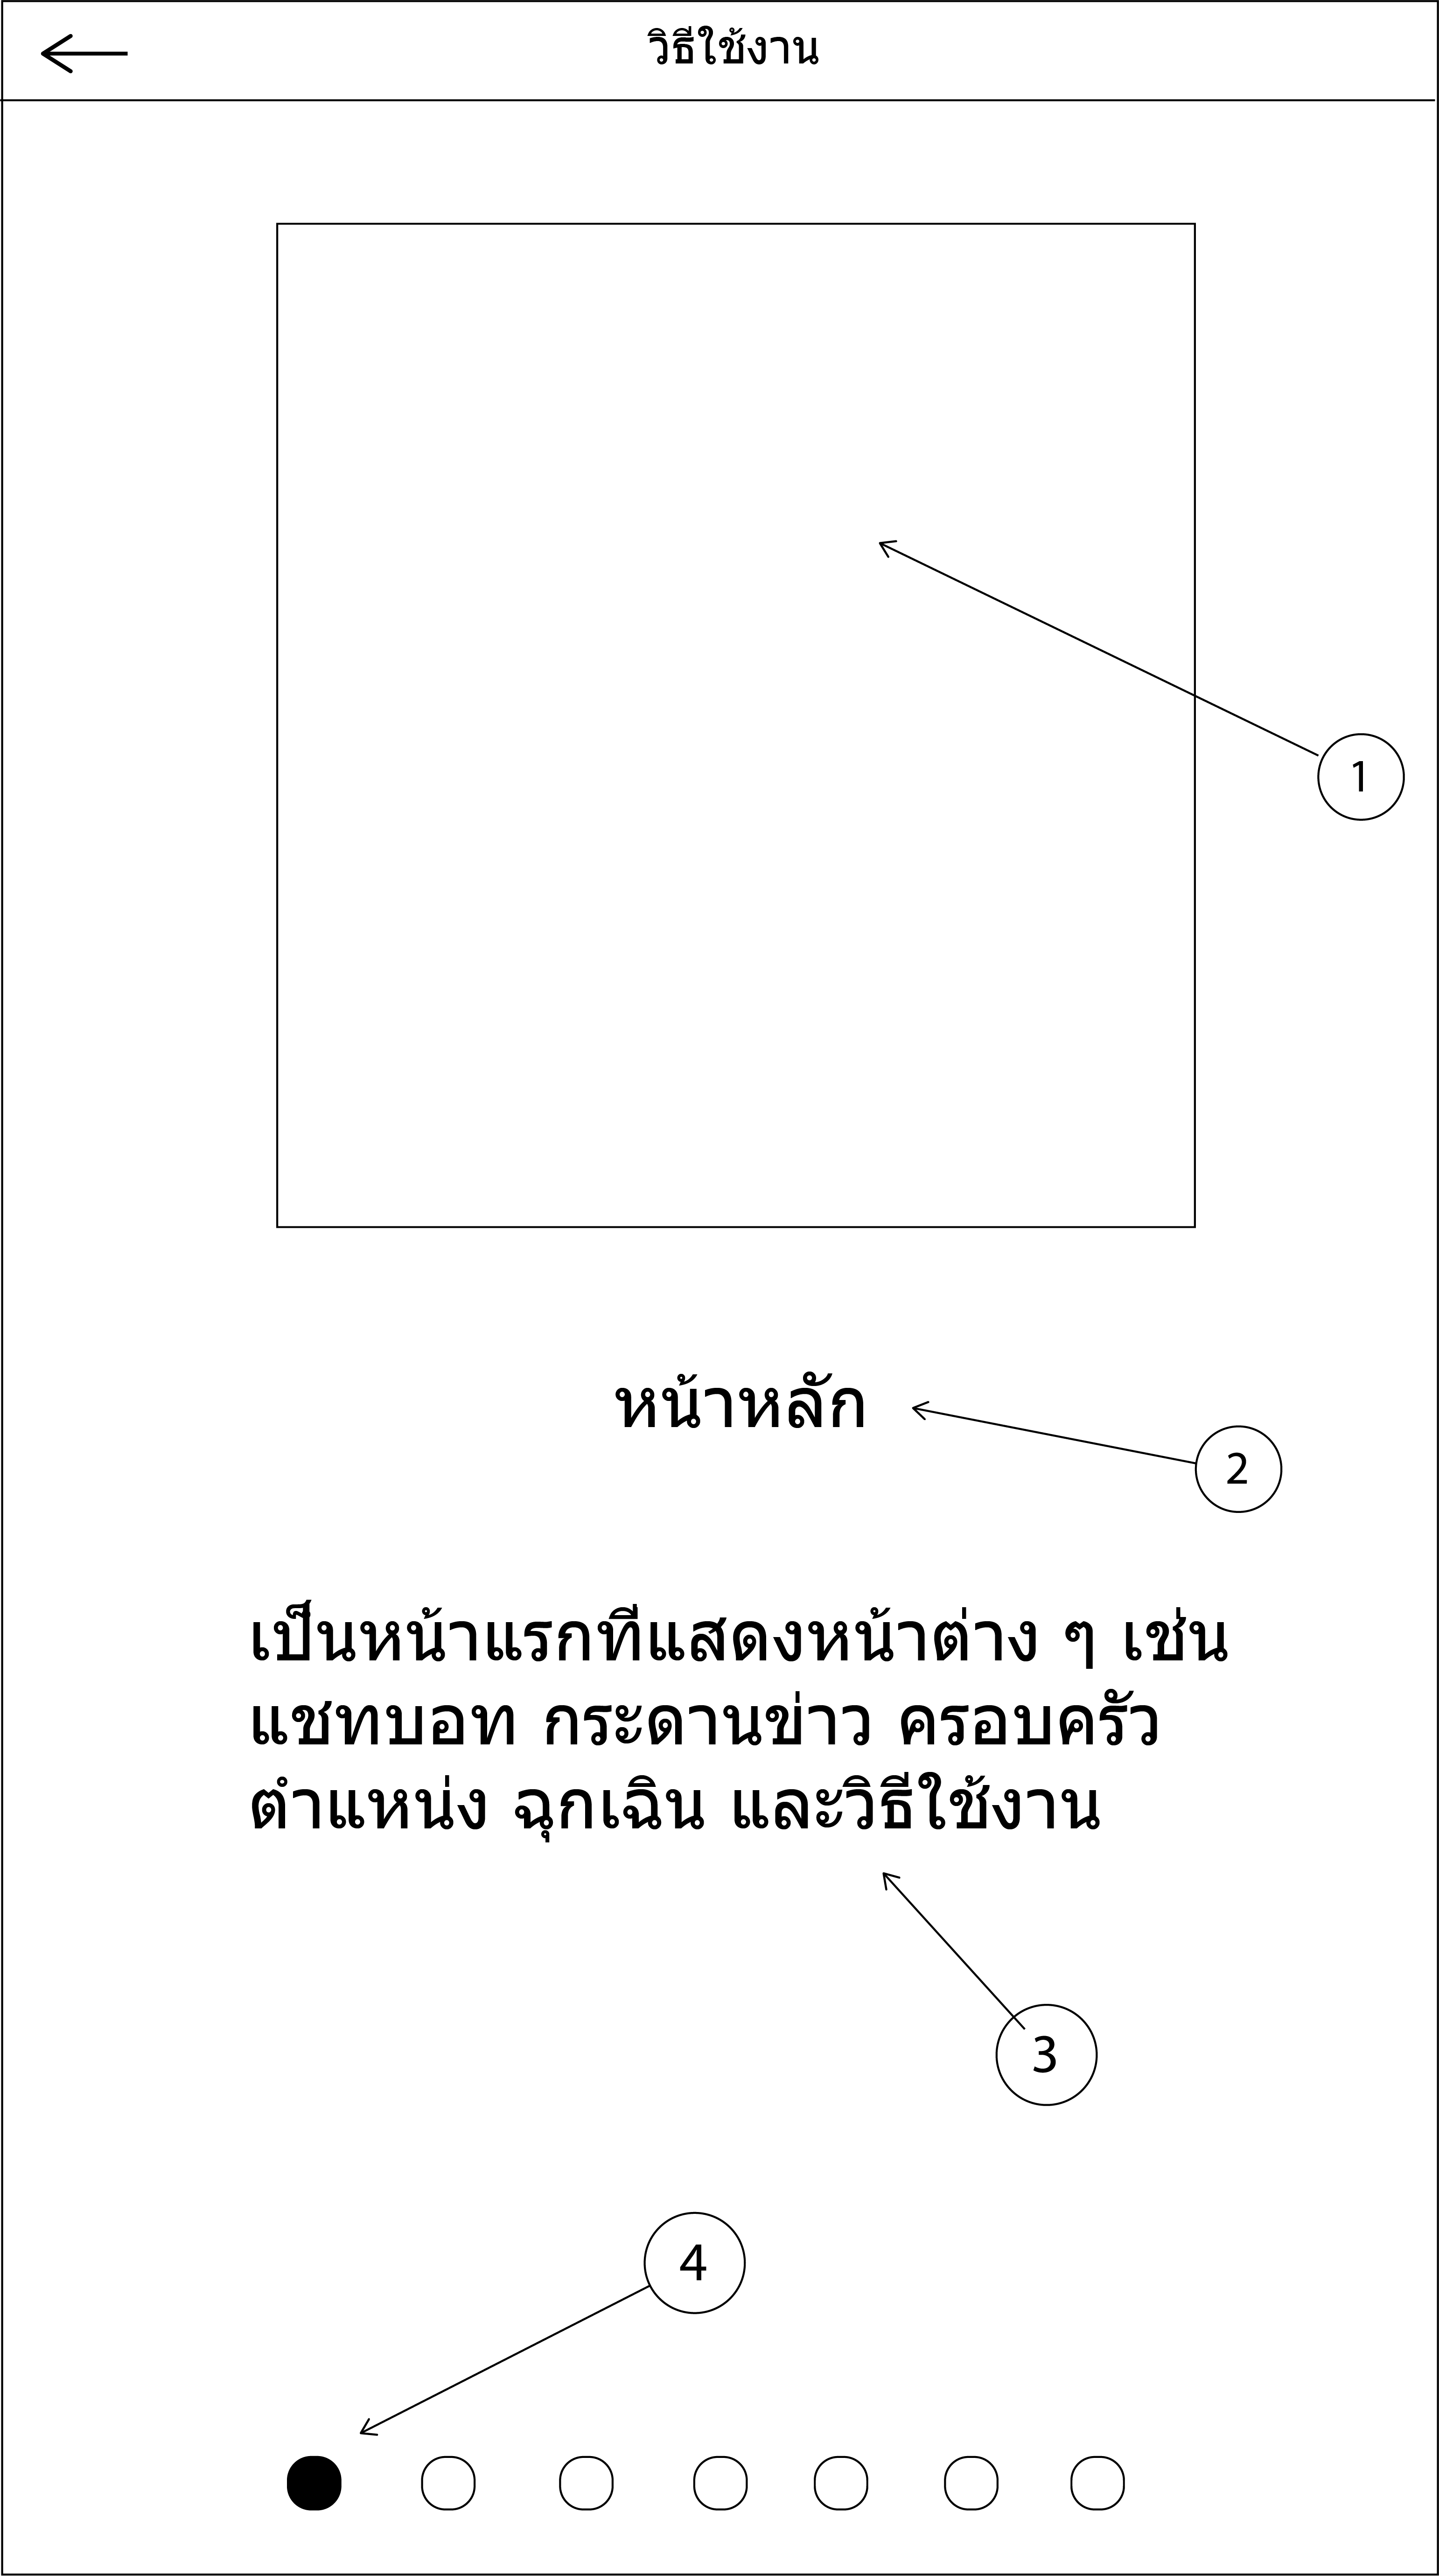
\includegraphics[width=0.6\textwidth]{Figures/3/UI/howto}
			\caption{หน้าวิธีใช้งาน}
			\label{Fig:วิธีใช้งาน}
		\end{figure}
		จากภาพที่ \ref{Fig:วิธีใช้งาน} การออกแบบหลักประกอบไปด้วย 4 ส่วนดังนี้
		\begin{itemize}
			\item ส่วนที่ 1 รูปภาพตัวอย่างแสดงหน้าจอนั้นๆ
			\item ส่วนที่ 2 ชือของหน้าจอนั้นๆ
			\item ส่วนที่ 3 รายละเอียดเพิ่มเติมของหน้าจอนั้นๆ
			\item ส่วนที่ 4 จุดสำหรับแสดงตำแหน่งที่เราอยู่ ณ ปัจจุบัน
		\end{itemize}

		\begin{figure}[H]
			\centering
			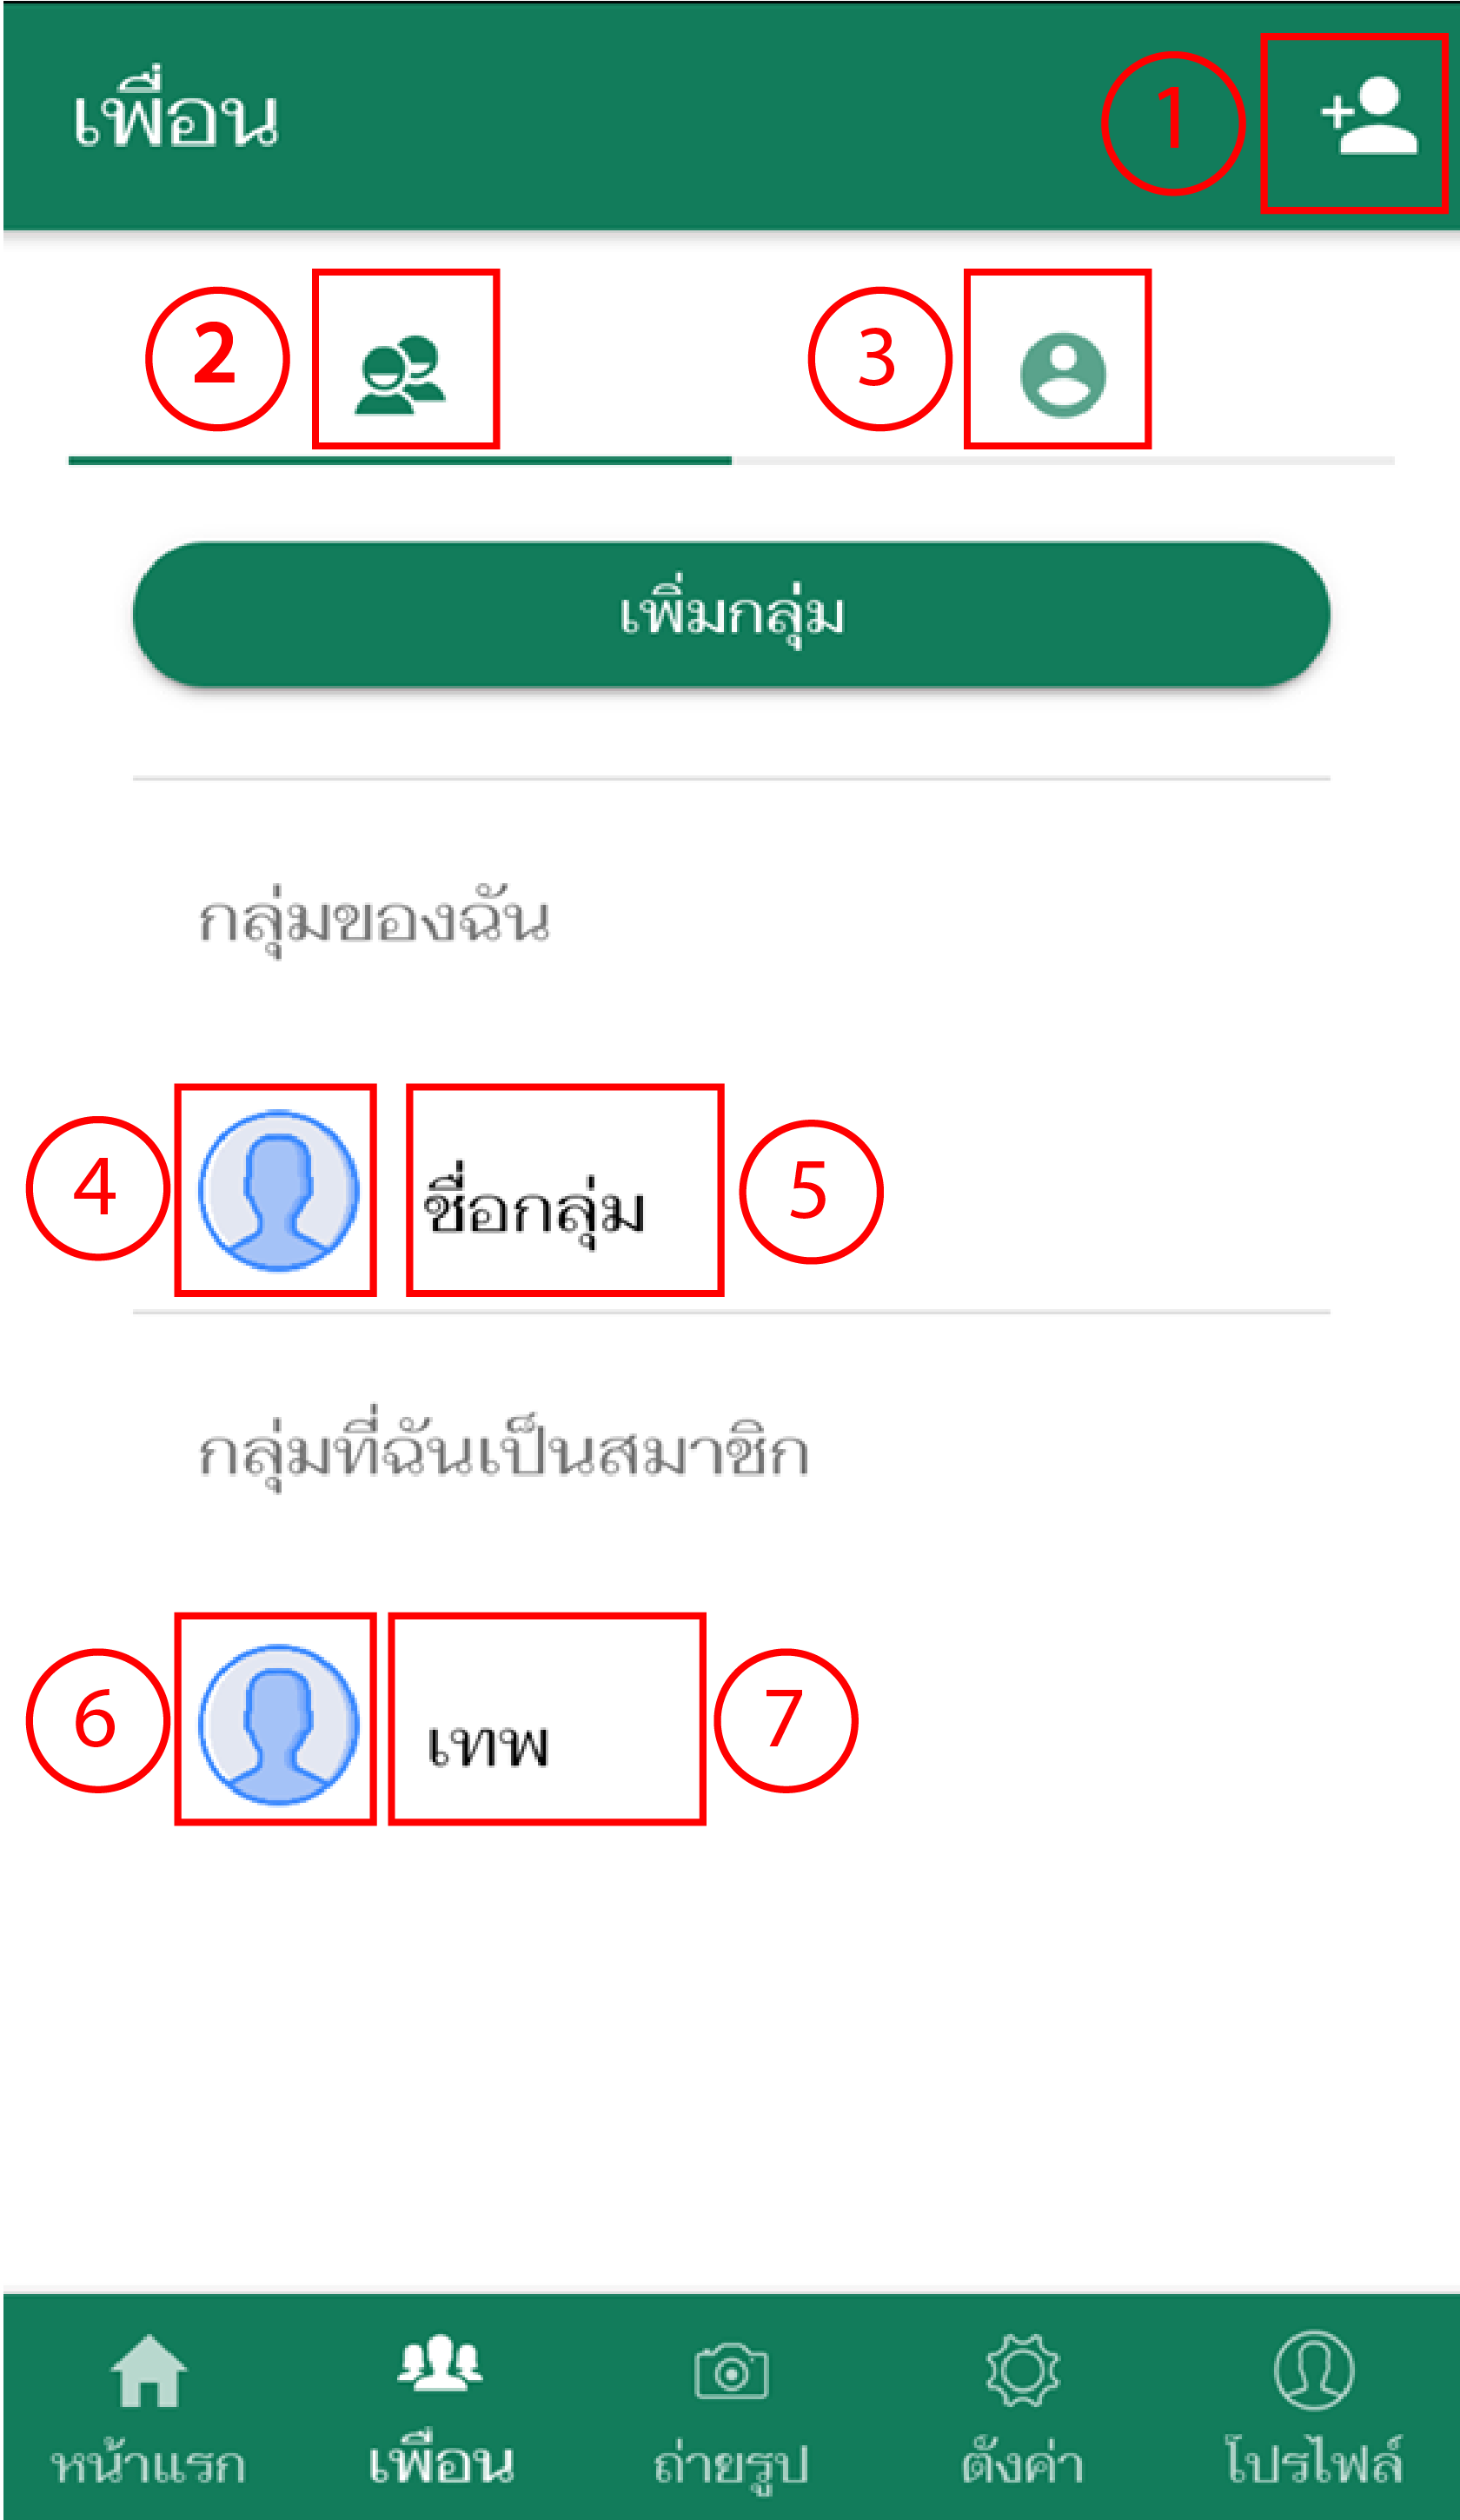
\includegraphics[width=0.6\textwidth]{Figures/3/UI/group}
			\caption{หน้าจอแสดงกลุ่ม}
			\label{Fig:กลุ่ม}
		\end{figure}
		จากภาพที่ \ref{Fig:กลุ่ม} การออกแบบหลักประกอบไปด้วย 7 ส่วนดังนี้
		\begin{itemize}
			\item ส่วนที่ 1 ปุ่มสำหรับเพิ่มเพื่อน
			\item ส่วนที่ 2 ปุ่มสำหรับไปยังหน้าแสดงกลุ่ม
			\item ส่วนที่ 3 ปุ่มสำหรับไปยังหน้าจอแสดงเพื่อน
			\item ส่วนที่ 4 รูปภาพของกลุ่มที่เราเป็นคนสร้าง
			\item ส่วนที่ 5 ชื่อของกลุ่มที่เราเป็นคนสร้าง
			\item ส่วนที่ 6 รูปภาพของกลุ่มที่เราเป็นสมาชิก
			\item ส่วนที่ 7 ชื่อของกลุ่มที่เราเป็นสมาชิก
		\end{itemize}

		\begin{figure}[H]
			\centering
			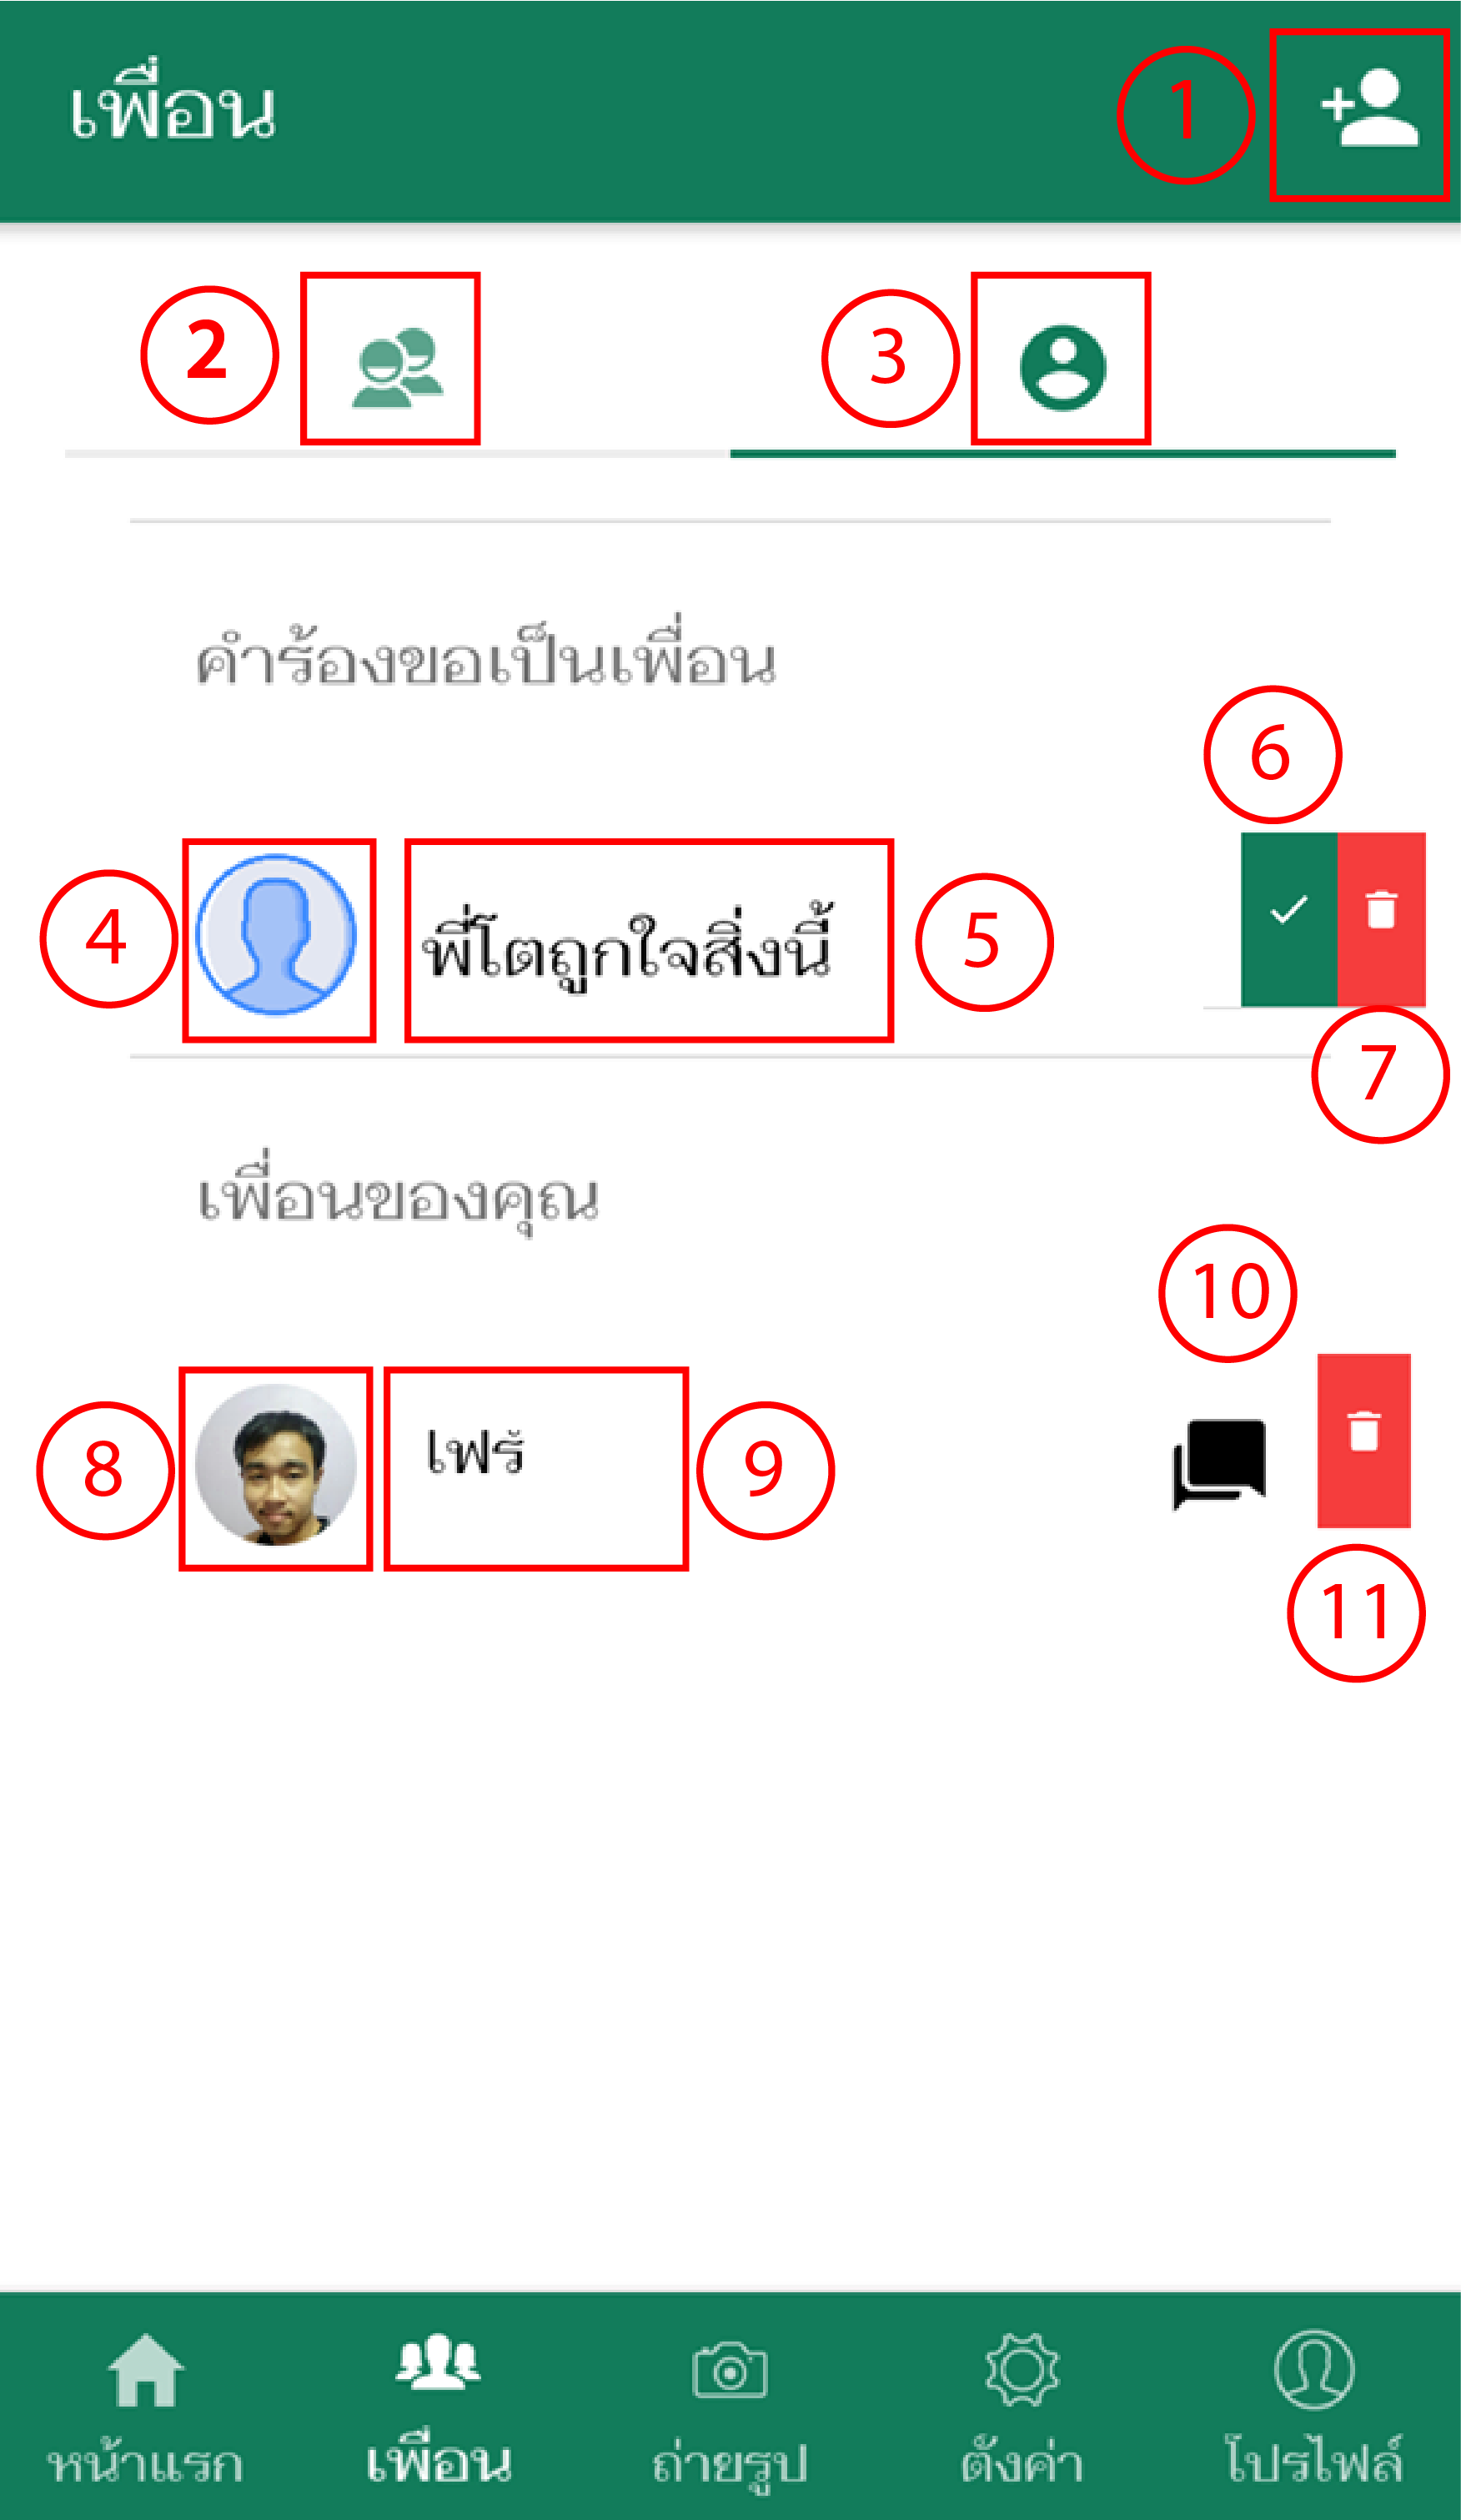
\includegraphics[width=0.6\textwidth]{Figures/3/UI/friend}
			\caption{หน้าจอแสดงเพื่อน}
			\label{Fig:เพื่อน}
		\end{figure}
		จากภาพที่ \ref{Fig:เพื่อน} การออกแบบหลักประกอบไปด้วย 8 ส่วนดังนี้
		\begin{itemize}
			\item ส่วนที่ 1 ปุ่มสำหรับเพิ่มเพื่อน
			\item ส่วนที่ 2 ปุ่มสำหรับไปยังหน้าแสดงกลุ่ม
			\item ส่วนที่ 3 ปุ่มสำหรับไปยังหน้าจอแสดงเพื่อน
			\item ส่วนที่ 4 รูปภาพของเพื่อนที่รอการยืนยัน
			\item ส่วนที่ 5 ชื่อของเพื่อนที่รอการยืนยัน
			\item ส่วนที่ 6 ปุ่มสำหรับยกเลิกคำขอร้องเป็นเพื่อน
			\item ส่วนที่ 7 รูปภาพของเพื่อน
			\item ส่วนที่ 8 ชื่อของเพื่อน
			\item ส่วนที่ 9 ปุ่มสำหรับแชทกับเพื่อน
			\item ส่วนที่ 10 ปุ่มสำหรับลบเพื่อน
		\end{itemize}

		\begin{figure}[H]
			\centering
			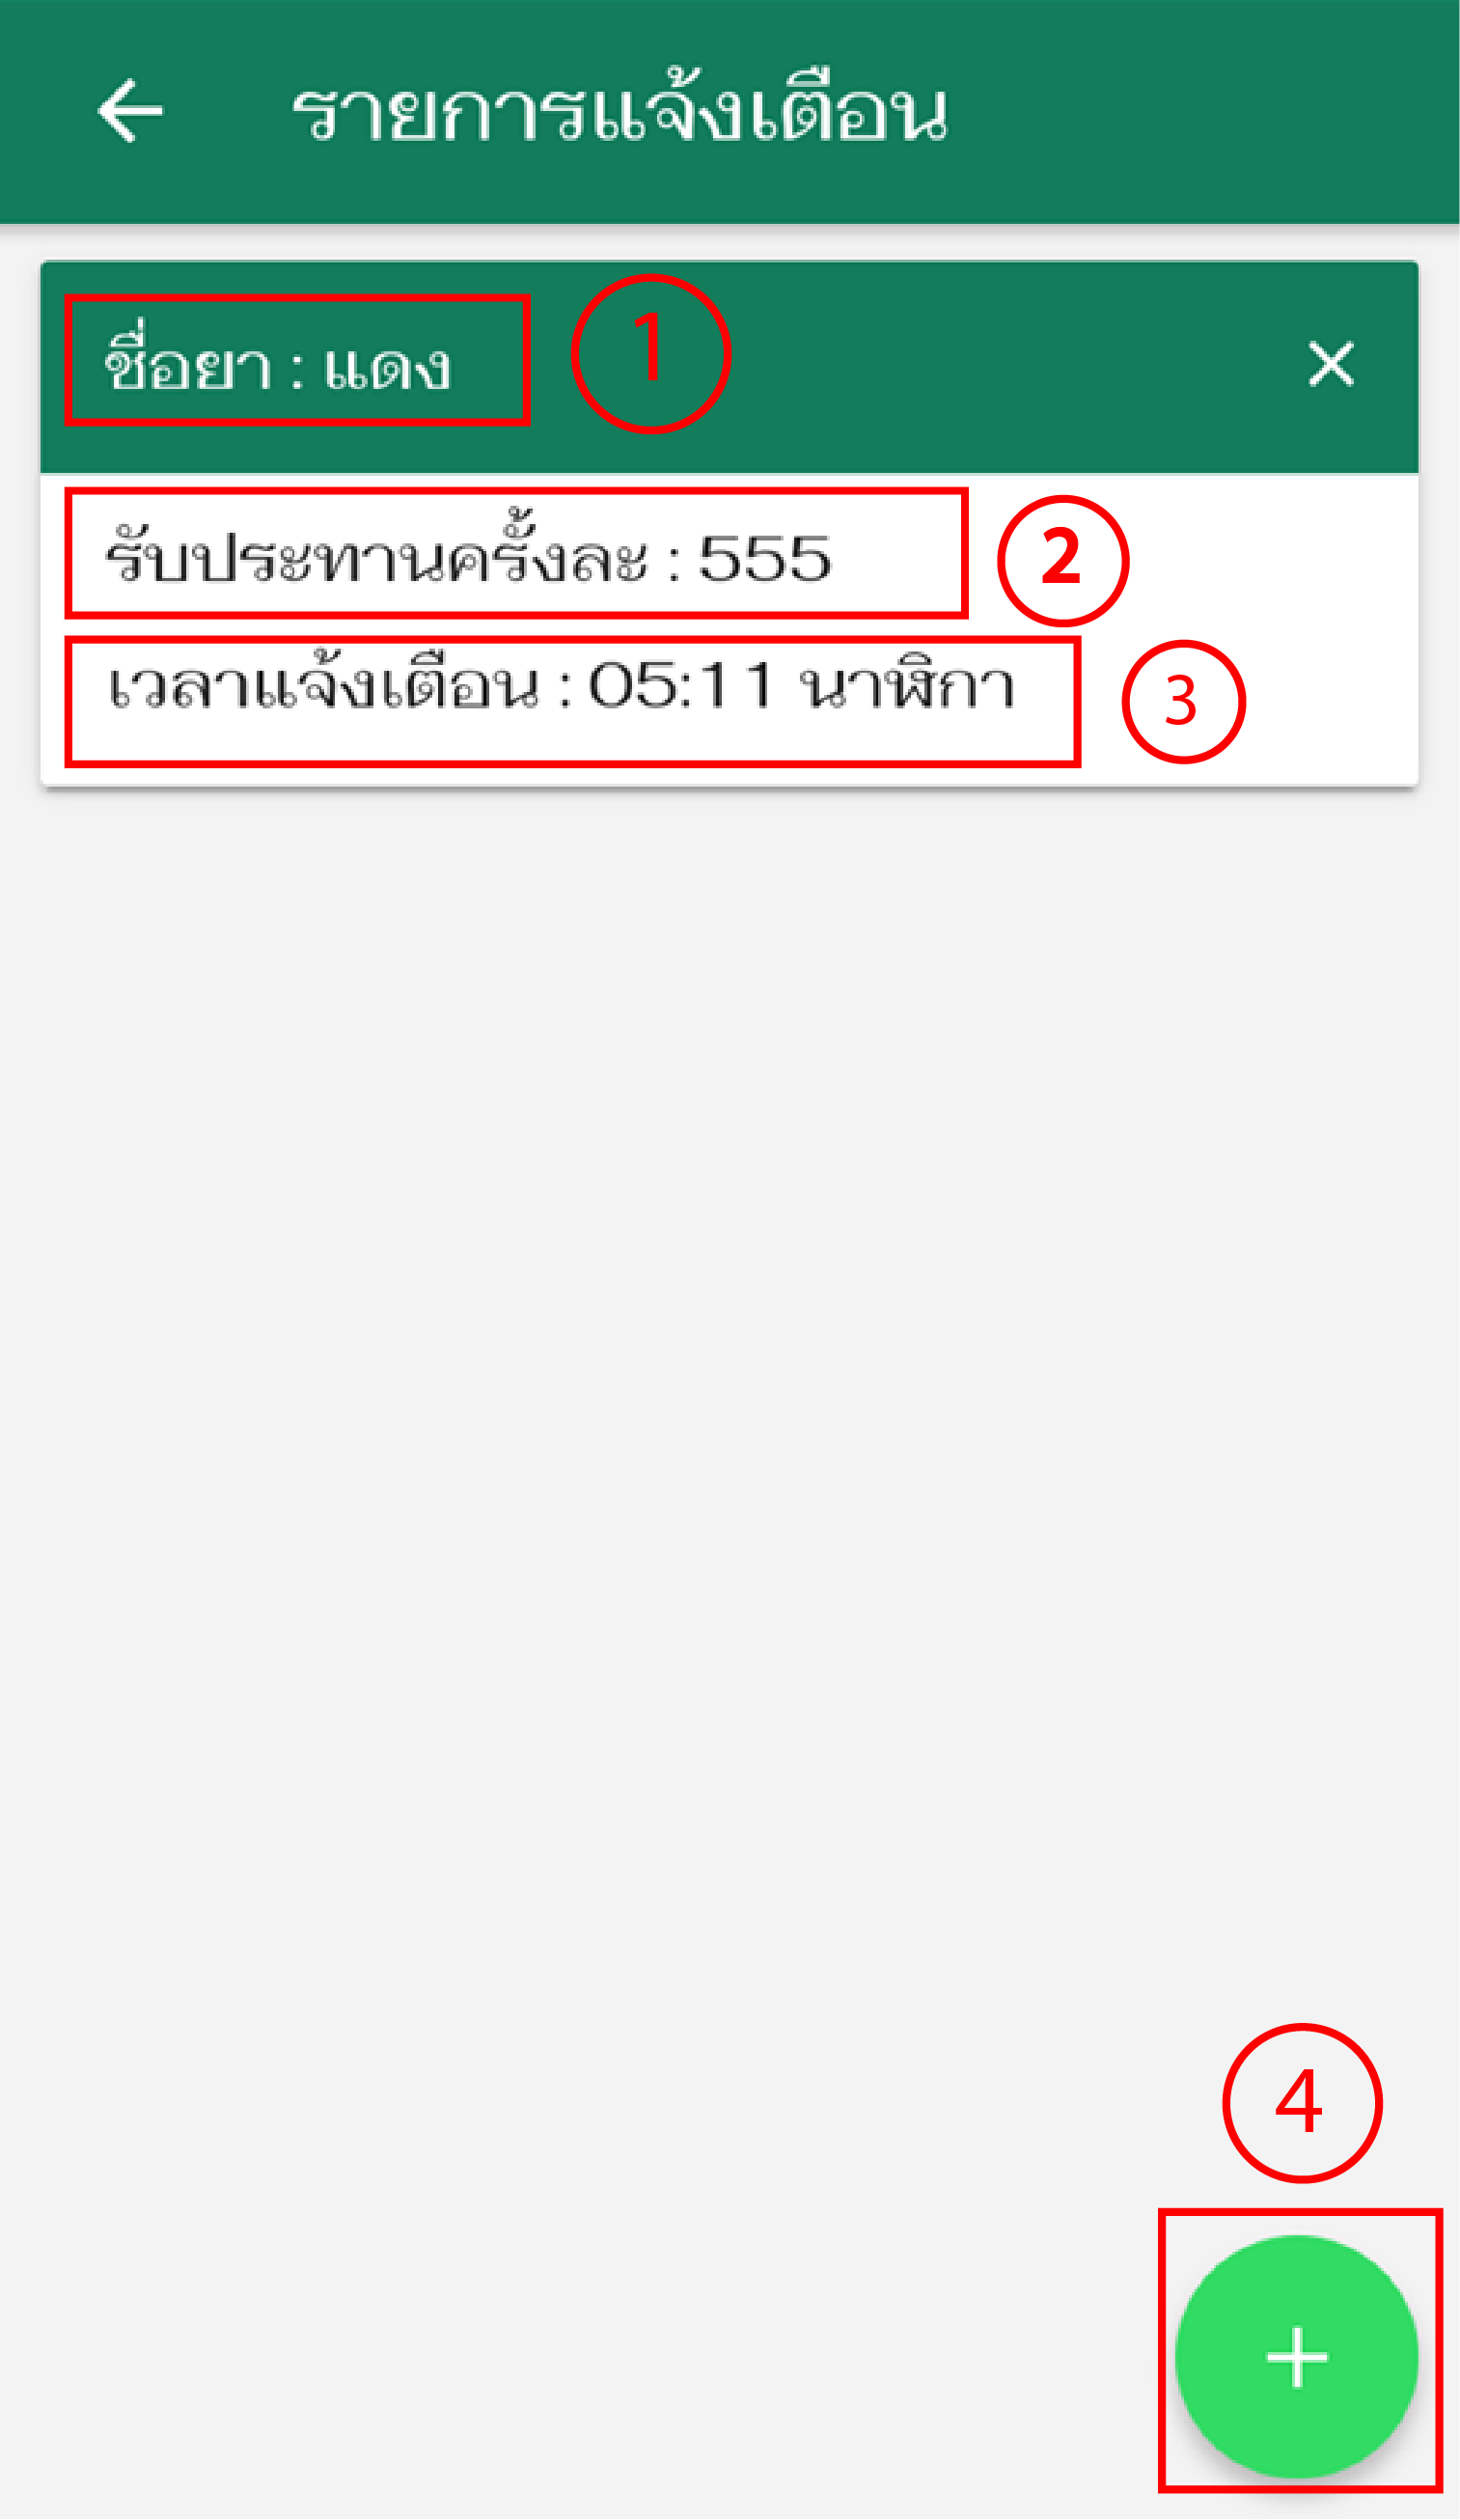
\includegraphics[width=0.6\textwidth]{Figures/3/UI/notification}
			\caption{หน้าแสดงรายการแจ้งเตือนการทานยา}
			\label{Fig:รายการทานยา}
		\end{figure}
		จากภาพที่ \ref{Fig:รายการทานยา} การออกแบบหลักประกอบไปด้วย 4 ส่วนดังนี้
		\begin{itemize}
			\item ส่วนที่ 1 ข้อความแสดงชื่อของยา
			\item ส่วนที่ 2 ข้อความแสดงจำนวนการรับประทานต่อครั้ง
			\item ส่วนที่ 3 ข้อความแสดงเวลาในการแจ้งเตือน
			\item ส่วนที่ 4 ปุ่มสำหรับเพิ่มการแจ้งเตือนการทานยา
		\end{itemize}

		\begin{figure}[H]
			\centering
			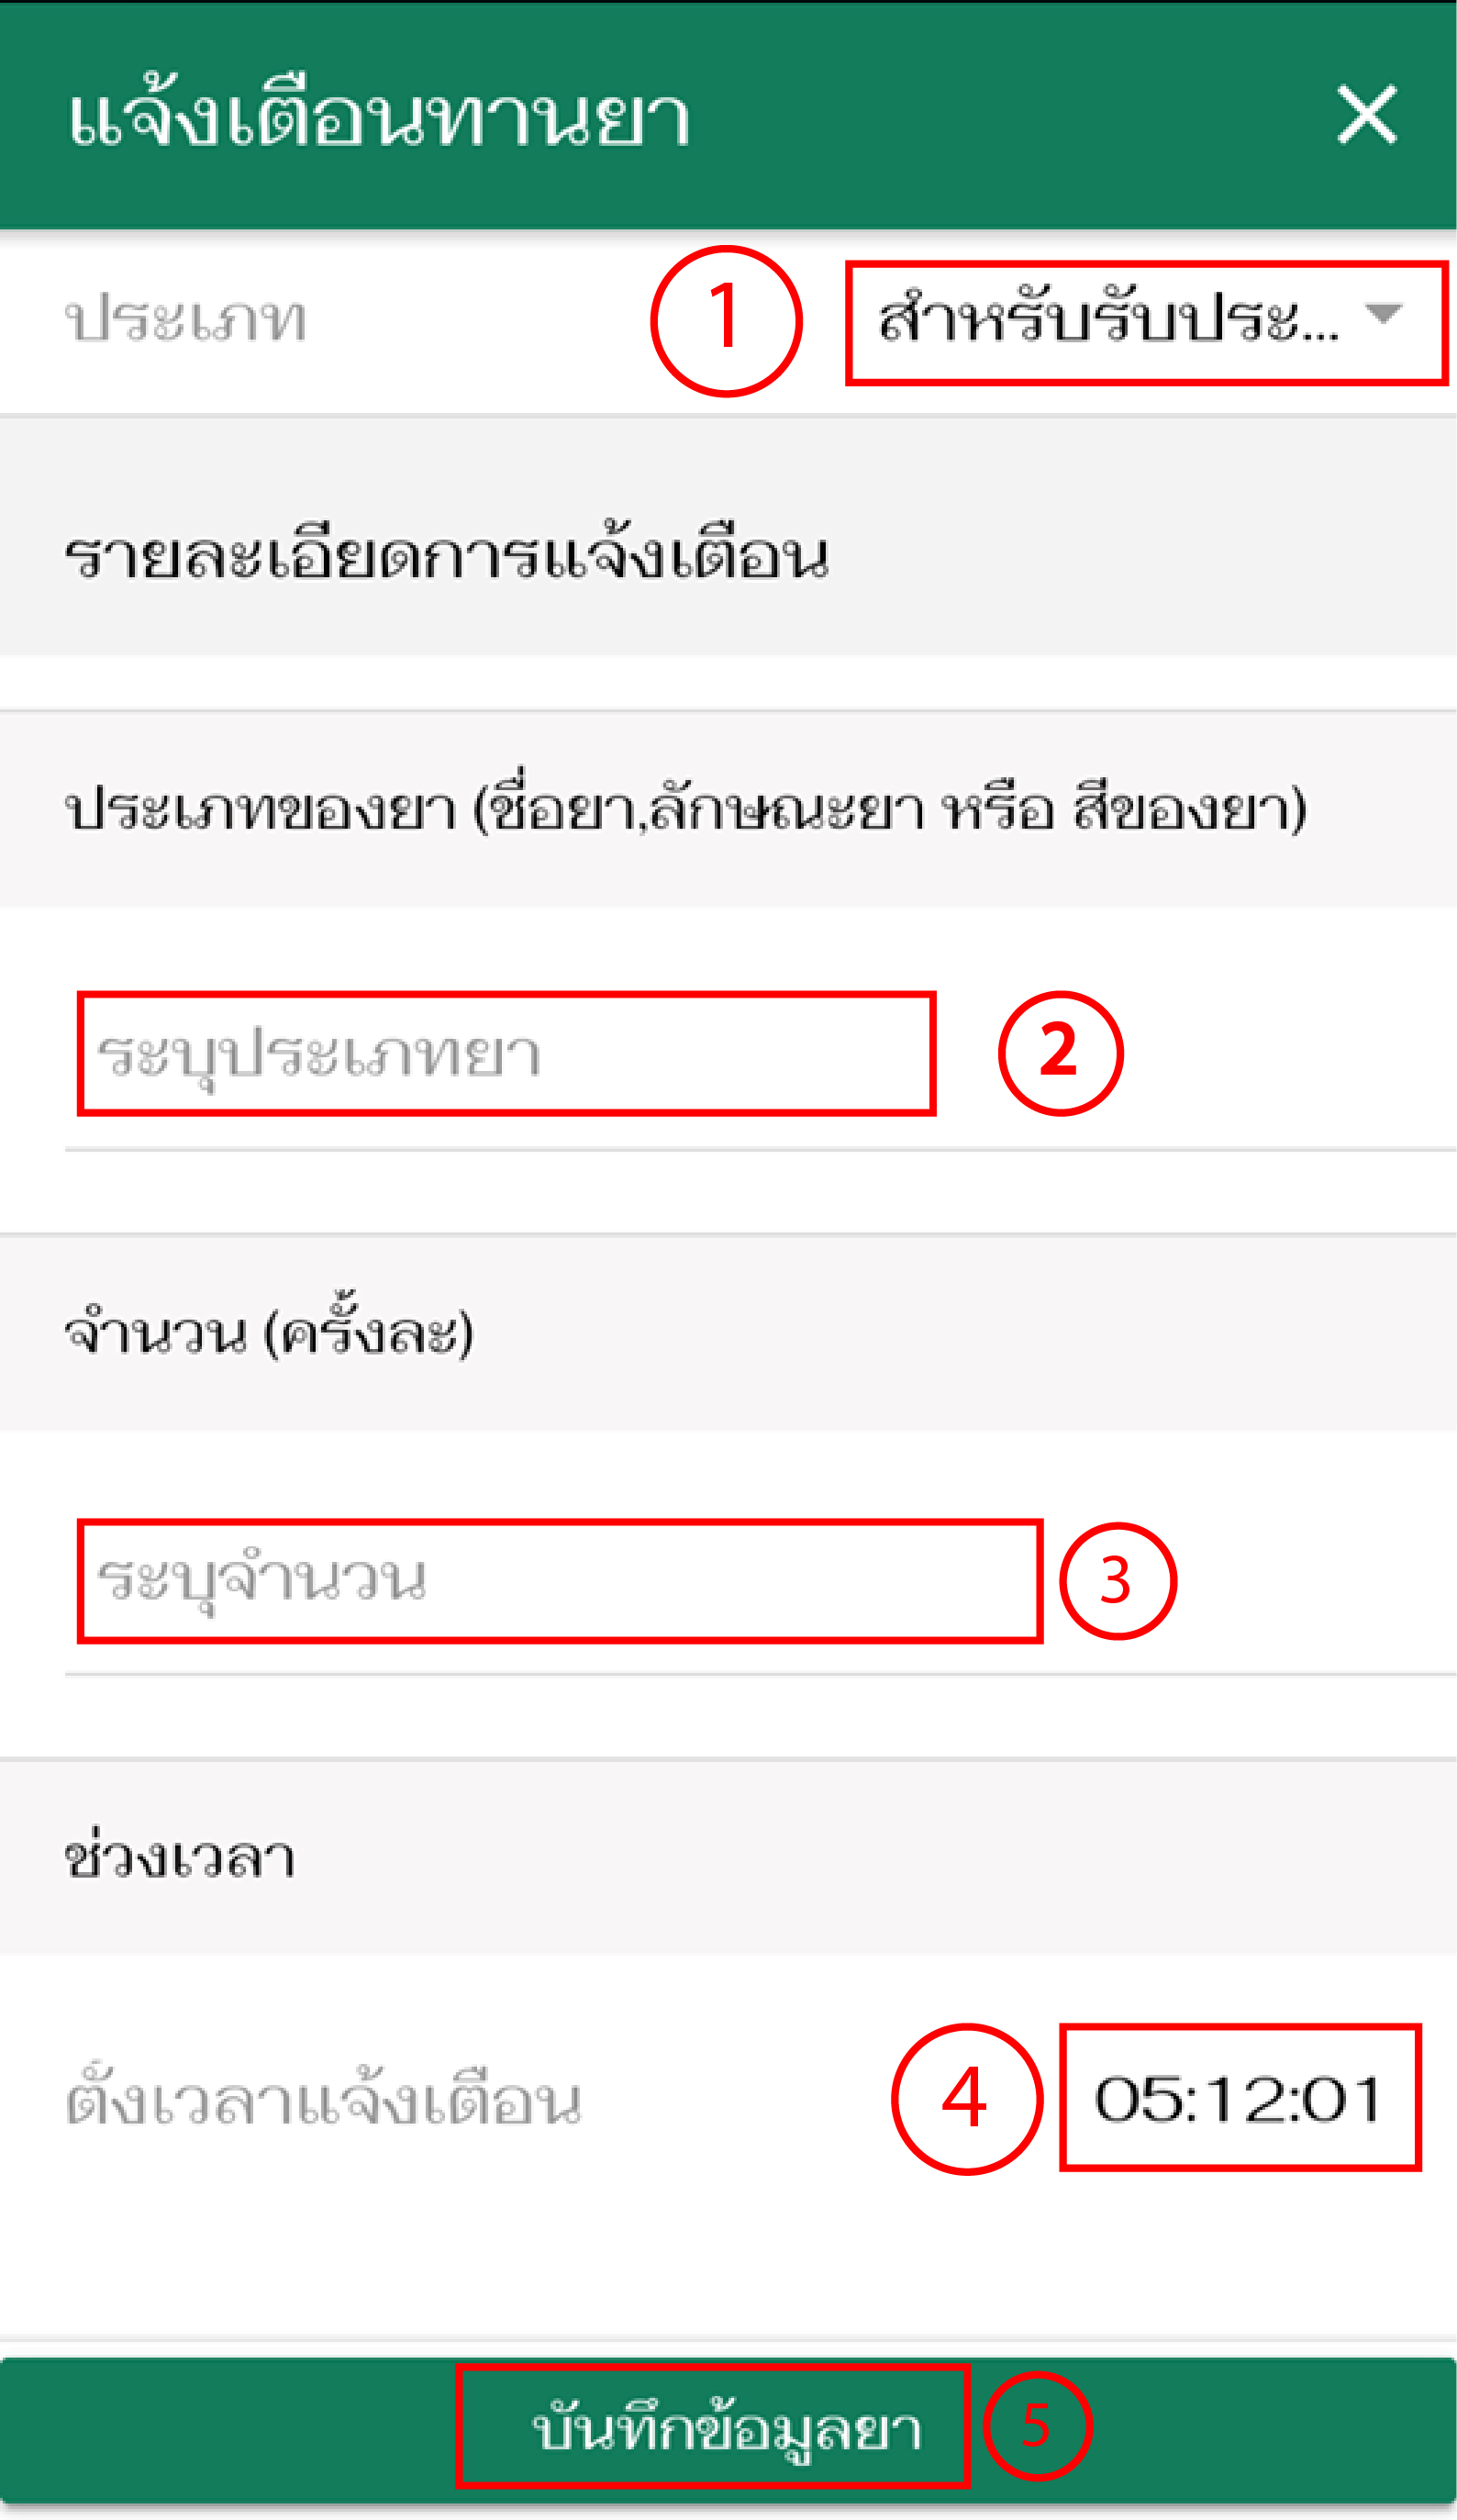
\includegraphics[width=0.6\textwidth]{Figures/3/UI/addnotification}
			\caption{หน้าแสดงการเพิ่มการแจ้งเตือนทานยา}
			\label{Fig:เพิ่มทานยา}
		\end{figure}
		จากภาพที่ \ref{Fig:เพิ่มทานยา} การออกแบบหลักประกอบไปด้วย 5 ส่วนดังนี้
		\begin{itemize}
			\item ส่วนที่ 1 ลิสท์สำหรับเลือกประเภทการรับประทานมี 2 ประเภทได้แก่ สำหรับรับประทานและสำหรับฉีด
			\item ส่วนที่ 2 ช่องสำหรับกรอกชื่อยา ลักษณะของยา หรือสีของยา
			\item ส่วนที่ 3 ช่องสำหรับกรอกจำนวนครั้งในการทานยา
			\item ส่วนที่ 4 ลิสท์สำหรับกำหนดเวลาการแจ้งเตือนการทานยา
			\item ส่วนที่ 5 ปุ่มสำหรับยืนยันการเพิ่มการแจ้งเตือนทานยา
		\end{itemize}

		\begin{figure}[H]
			\centering
			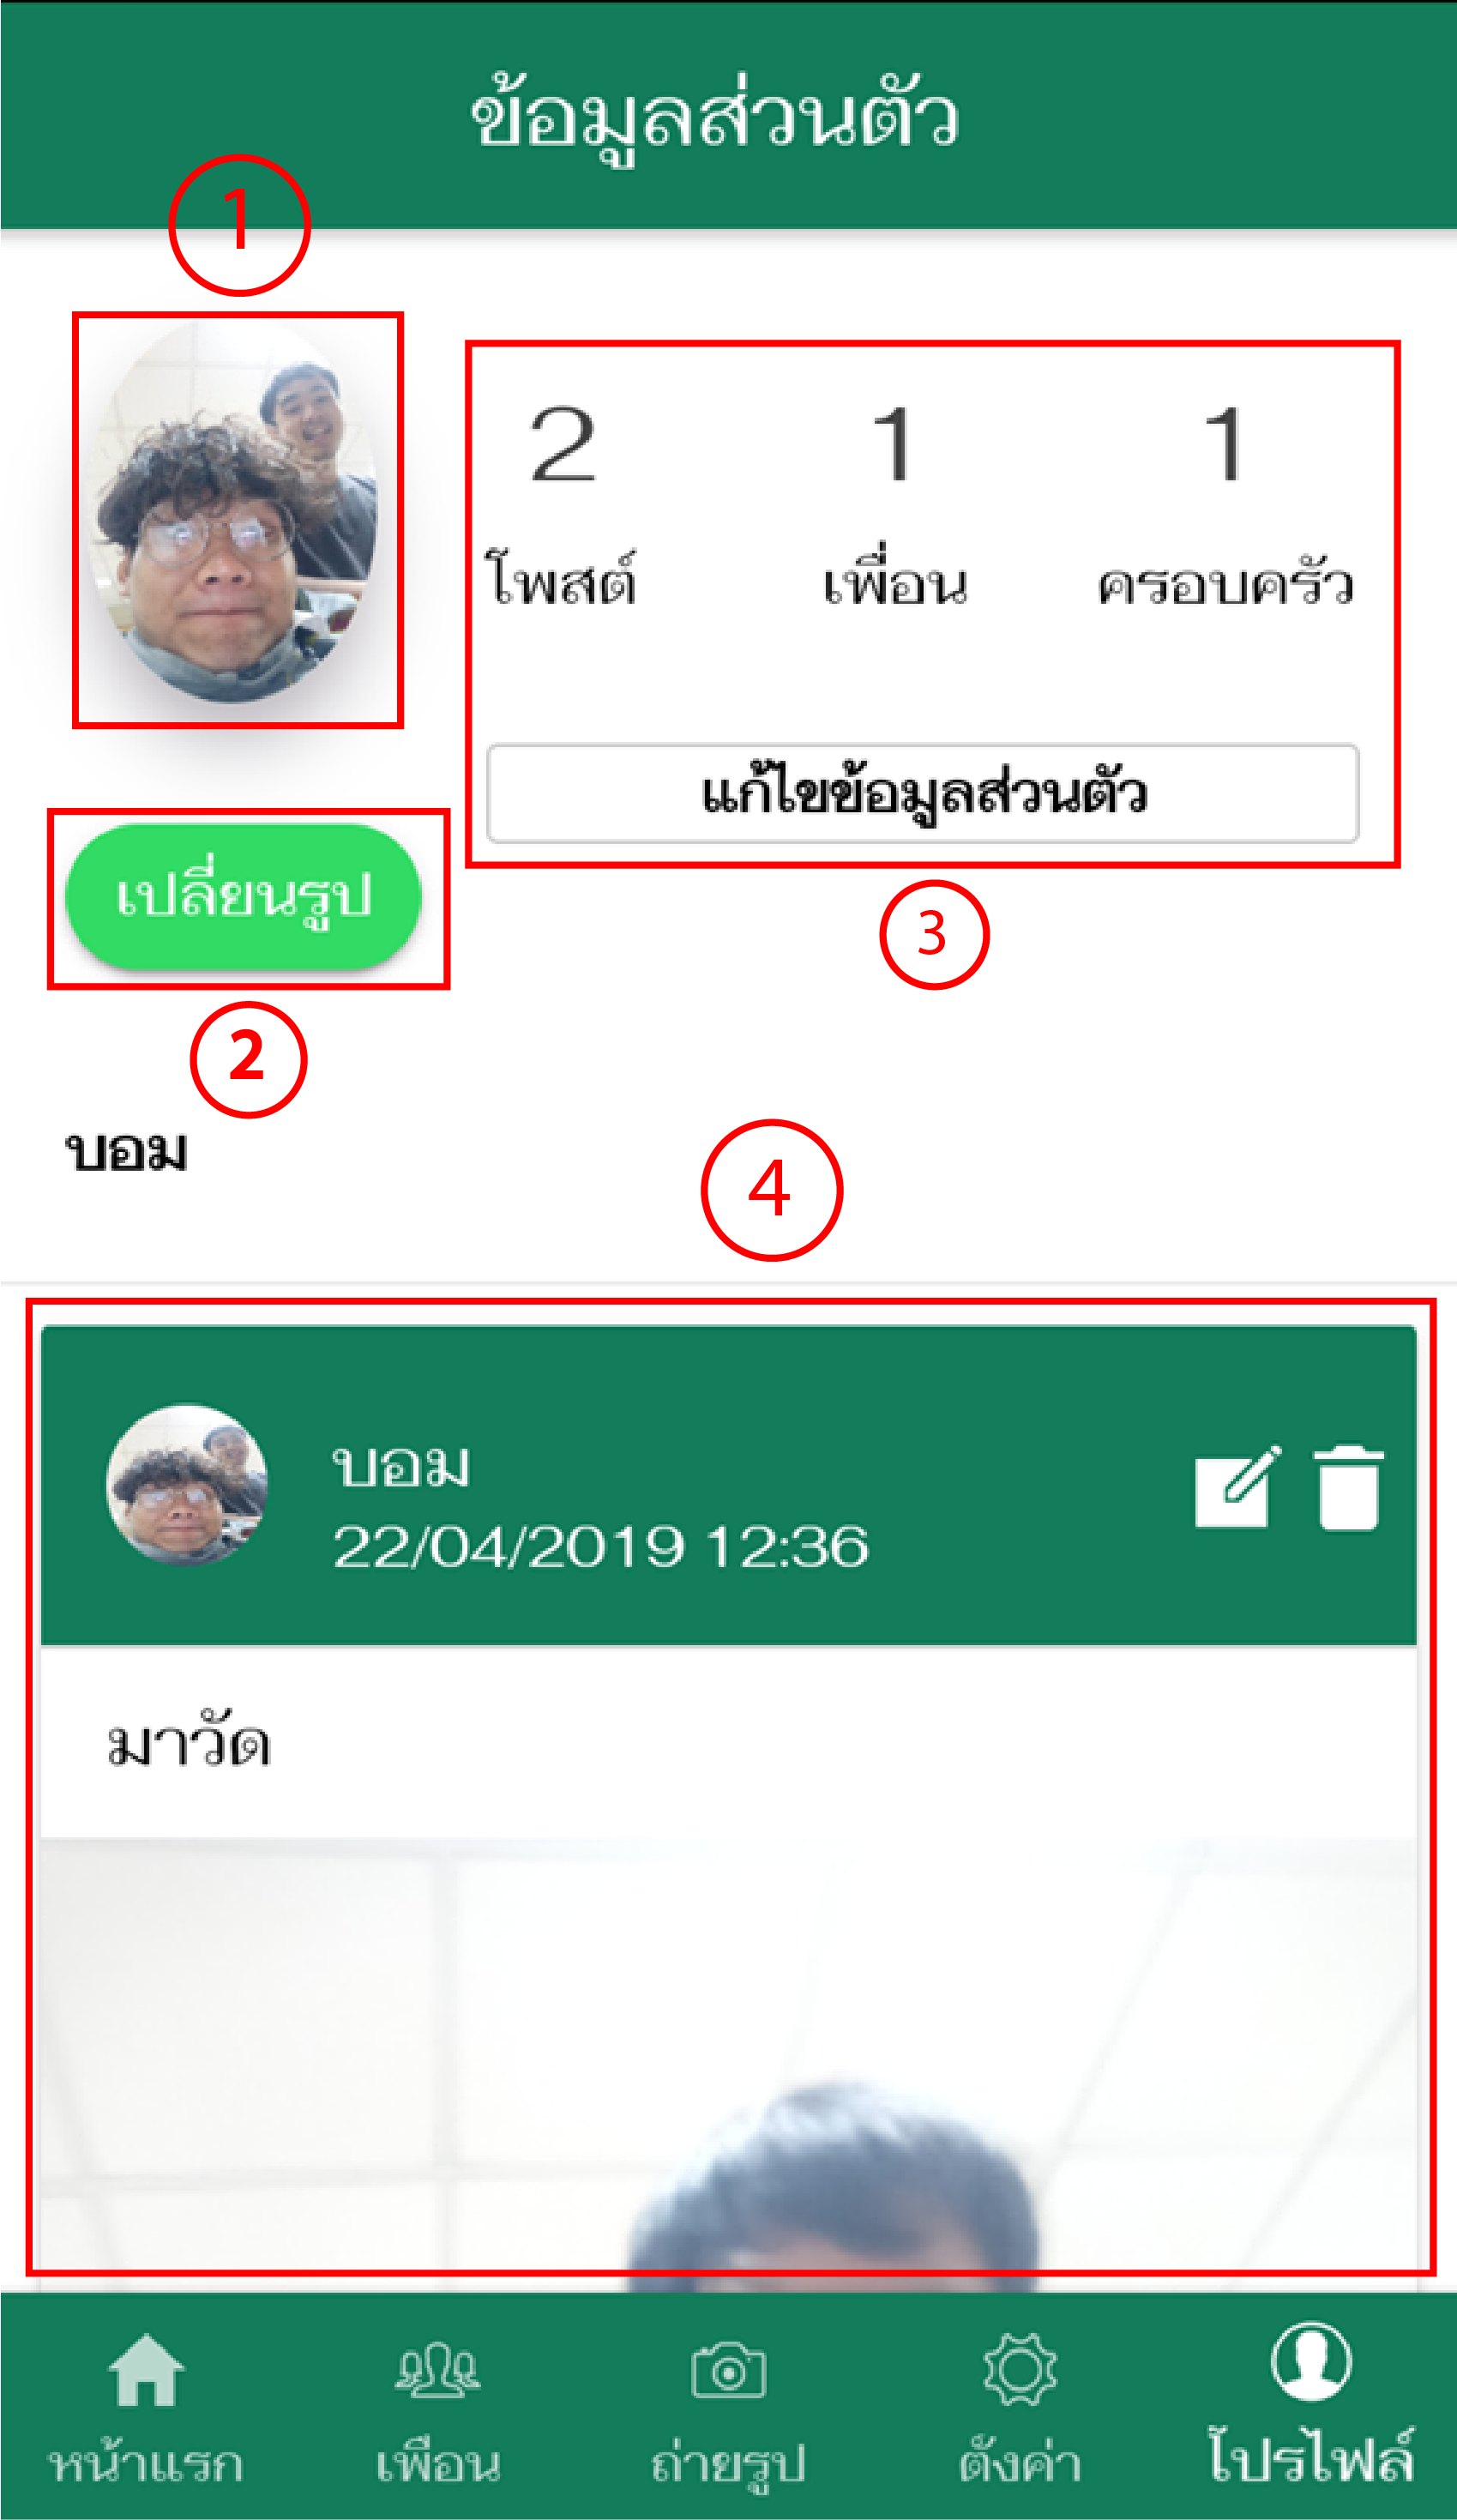
\includegraphics[width=0.6\textwidth]{Figures/3/UI/profile}
			\caption{หน้าจอแสดงข้อมูลส่วนตัวของผู้ใช้}
			\label{Fig:โปรไฟล์}
		\end{figure}
		จากภาพที่ \ref{Fig:โปรไฟล์} การออกแบบหลักประกอบไปด้วย 4 ส่วนดังนี้
		\begin{itemize}
			\item ส่วนที่ 1 รูปประจำตัวของผู้ใช้
			\item ส่วนที่ 2 ปุ่มสำหรับเปลี่ยนรูปประจำตัว
			\item ส่วนที่ 3 แสดงจำนวนโพสท์ เพื่อน ครอบครัว และปุ่มแก้ไขข้อมูลส่วนตัว
			\item ส่วนที่ 4 โพสท์ของผู้ใช้
		\end{itemize}
\newpage

%  สิ้นสุด User Interface Design

%  เริ่มต้น Diagram

\section{แผนภาพไดอะแกรม}

%  เริ่มต้น Use Case Diagram

\subsection{แผนภาพยูสเคส (Use Case Diagram)}
	Use Case Diagram เป็นแผนผังเพื่อแสดงฟังก์ชันแสดงการทำงานของระบบโดยรวม แสดงส่วนประกอบในระบบและกิจกรรมที่เกิดขึ้นในระบบซึ่งในระบบระบบกองทุนเงินให้กู้ยืมเพื่อการศึกษา คณะวิทยาศาสตร์ มหาวิทยาลัยอุบลราชธานี ผู้ใช้จำเป็นต้องเข้าสู่ระบบเพื่อใช้งานระบบ สัญลักษณ์ที่ใช้ในการเขียน Use Case Diagram แสดงในตารางที่ \ref{tab:use-case2}
	\begin{table}[H]
		\caption{สัญลักษณ์ของ Use case Diagram}
		\label{tab:use-case2}
		\begin{tabular}{|c|p{10cm}|}
		\hline
		\textbf{สัญลักษณ์} & \multicolumn{1}{c|}{\textbf{การใช้งาน}} \\ \hline
		\raisebox{-\totalheight}{Use case}
		& \setstretch{1.5} {Use case คือส่วนย่อยของระบบงาน แทนด้วยวงรีและชื่อของ Use case ภายในวงรี} \\ \hline
		\raisebox{-\totalheight}{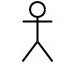
\includegraphics[height=1.5cm]{Figures/table/use-case/2}}
		& \setstretch{1.5} {Actor คือบุคคลหรือระบบงานอื่นที่ใช้งานระบบหรือได้รับประโยชน์จากระบบซึ่งอยู่ภายนอกระบบ แทนด้วยรูปคนและมีชื่อบทบาทการใช้งานระบบ} \\ \hline
		\raisebox{-\totalheight}{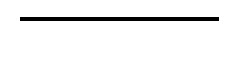
\includegraphics[width=3cm]{Figures/table/use-case/3}}
		& \setstretch{1.5} {เส้นตรงที่แสดงถึงการใช้งาน Use case ของผู้กระทำ} \\ \hline
		\raisebox{-\totalheight}{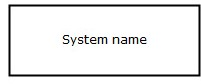
\includegraphics[width=0.3\textwidth]{Figures/table/use-case/4}}
		& \setstretch{1.5} {กรอบสี่เหลี่ยมแสดงถึงขอบเขตของระบบโดยแสดงชื่อระบบภายในหรือด้านบนกรอกสี่เหลี่ยม Use case อยู่ภายในกรอบสี่เหลี่ยม และ actor อยู่ภายนอกกรอบสี่เหลี่ยม} \\ \hline
		\raisebox{-\totalheight}{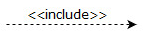
\includegraphics[width=0.3\textwidth]{Figures/table/use-case/5}}
		& \setstretch{1.5} {ความสัมพันธ์แบบ <<includes>> แสดงว่า Use case หนึ่งดำเนินการตามขั้นตอนของ Use case อื่น โดยแทนด้วยสัณลักษณ์ลูกศรเส้นประ ซึ่ง Use case ที่หางลูกศรเรียกใช้งาน Use case ที่หัวลูกศรทุกครั้งที่มีการทำงาน} \\ \hline
		\raisebox{-\totalheight}{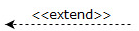
\includegraphics[width=0.3\textwidth]{Figures/table/use-case/6}}
		& \setstretch{1.5} {ความสัมพันธ์แบบ <<extend>> แสดงว่า Use case หนึ่งดำเนินการตามขั้นตอนของ Use case อื่น โดยแทนด้วยสัญลักษณ์ลูกศรเส้นประ ซึ่ง Use case ที่หัวลูกศรเรียกใช้งาน Use case ที่หางลูกศร แต่การใช้งานไม่จำเป็นต้องเกิดขึ้นทุกครั้งขึ้นอยู่กับเงื่อนไขระหว่างการทำงาน} \\ \hline
		\end{tabular}
	\end{table}

	\begin{figure}[H]
		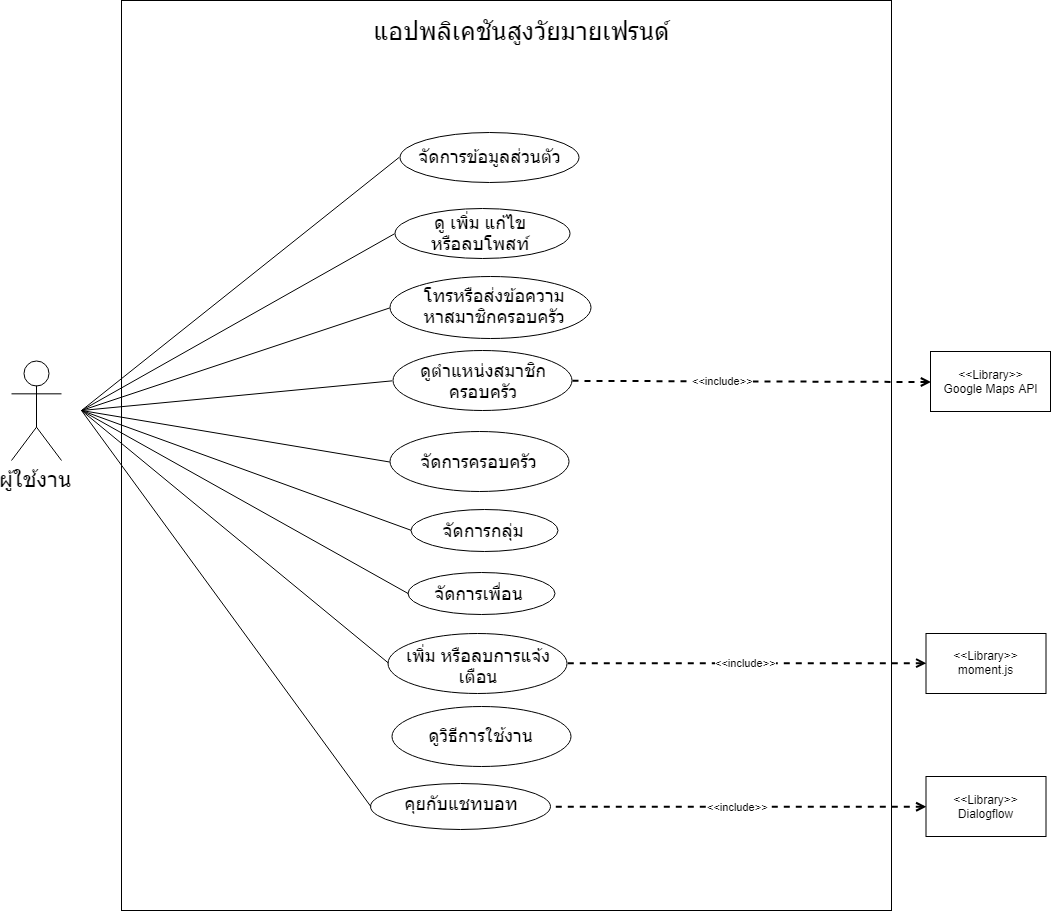
\includegraphics[width=1.1\textwidth]{Figures/3/Usecase/Usecase}
		\caption{Use Case Diagram ของแอปพลิเคชันสูงวัยมายเฟรนด์}
		\label{Fig:usecase}
	\end{figure}
	
	\begin{table}[H]
		\centering
		\caption{อธิบาย Use Case หน้าที่ของแอปพลิเคชันสูงวัยมายเฟรนด์ในภาพที่ \ref{Fig:usecase}}
		\label{tab:usecase}
		\resizebox{\totalheight}{!}{\columnwidth}{%
			\begin{tabular}{|c|p{10cm}|}
				\hline
				\multicolumn{1}{|c|}{\textbf{Use Case}} & \multicolumn{1}{c|}{\textbf{คำอธิบาย}} \\ \hline
				เข้าสู่ระบบ & ใช้สำหรับให้ผู้ใช้เข้าใช้งานแอปพลิเคชัน \\ \hline
				ออกจากระบบ & ผู้ใช้ที่เข้าสู่ระบบแล้วสามารถออกจากระบบ \\ \hline
				จัดการข้อมูลส่วนตัว & ใช้งานเพื่อให้ผู้ใช้ แก้ไขข้อมูลที่ต้องการเปลี่ยนแปลง \\ \hline
				ดู เพิ่ม แก้ไข หรือลบโพสท์ & ใช้งานเพื่อให้ผู้ใช้สามารถดู เพิ่ม แก้ไข หรือลบโพสท์ของตัวเอง \\ \hline
				โทรหรือส่งข้อความหาสมาชิกในครอบครัว & ใช้สำหรับให้ผู้ใช้สามารถโทรหรือส่งข้อความหาคนในครอบครัว และสามารถเปิดเสียงฉุกเฉิน \\ \hline
				ดูตำแหน่งสมาชิกในครอบครัว & ใช้งานเพื่อให้ผู้ใช้สามารถดูตำแหน่งปัจจุบันของสมาชิกในครอบครัวด้วยแผนที่ \\ \hline
				จัดการครอบครัว & ใช้สำหรับเพิ่ม แก้ไข หรือลบข้อมูลสมาชิกครอบครัว \\ \hline
				จัดการกลุ่ม & ใช้สำหรับเพิ่ม แชท แก้ไข หรือลบกลุ่มได้ และเพิ่ม แก้ไข หรือลบสมาชิกในกลุ่มได้ \\ \hline
				จัดการเพื่อน & ใช้สำหรับยืนยันคำร้องขอเป็นเพื่อน รวมถึงพูดคุย เพิ่มและลบเพื่อน \\ \hline
				เพิ่ม หรือลบการแจ้งเตือน & ใช้สำหรับเพิ่ม หรือลบการแจ้งเตือนการทานยา \\ \hline
				ดูวิธีการใช้งาน & ใช้สำหรับให้ผู้ใช้ดูรายละเอียดของหน้าต่าง ๆ ในแอปพลิเคชัน \\ \hline
				คุยกับแชทบอท & ใช้งานเพื่อให้ผู้ใช้สามารถถามเรื่องโรคหรือเรื่องที่สนใจ \\ \hline
			\end{tabular}%
		}
	\end{table}

	\begin{table}[H]
		\centering
		\caption{Use Case เข้าสู่ระบบ}
		\label{tab:usecase}
		\resizebox{\totalheight}{!}{\textwidth}{%
			\begin{tabular}{|p{10cm}|p{10cm}|}
				\hline
				\textbf{Use Case Title : เข้าสู่ระบบ} & \multicolumn{1}{|c|}{\textbf{Use case Id : 1 }} \\ \hline
				\multicolumn{2}{|p{\linewidth}|}{Primary Actor : ผู้ใช้งาน} \\ \hline
			    \multicolumn{2}{|p{\linewidth}|}{Stakeholder Actor : -} \\ \hline
			    \multicolumn{2}{|p{\linewidth}|}{Main Flow : สามารถเข้าสู่ระบบเพื่อใช้งานแอปพลิเคชัน} \\ \hline
				\multicolumn{2}{|p{\linewidth}|}{Exceptional Flow ที่ 1 : หากผู้ใช้ไม่เชื่อมต่ออินเทอร์เน็ต จะไม่สามารถเข้าสู่ระบบได้} \\ \hline
			\end{tabular}%
		}
	\end{table}
	\begin{table}[H]
		\centering
		\caption{Use Case ออกจากระบบ}
		\label{tab:usecase}
		\resizebox{\totalheight}{!}{\textwidth}{%
			\begin{tabular}{|p{10cm}|p{10cm}|}
				\hline
				\textbf{Use Case Title : ออกจากระบบ} & \multicolumn{1}{|c|}{\textbf{Use case Id : 2 }} \\ \hline
				\multicolumn{2}{|l|}{Primary Actor : ผู้ใช้งาน} \\ \hline
				\multicolumn{2}{|l|}{Stakeholder Actor : -} \\ \hline
				\multicolumn{2}{|p{\linewidth}|}{Main Flow : สามารถออกจากระบบได้} \\ \hline
				\multicolumn{2}{|p{\linewidth}|}{Exceptional Flow ที่ 1 : หากยังไม่เข้าสู่ระบบจะไม่สามารถออกจากระบบได้} \\ \hline
			\end{tabular}%
		}
	\end{table}

	\begin{table}[H]
		\centering
		\caption{Use Case จัดการข้อมูลส่วนตัว}
		\label{tab:usecase}
		\resizebox{\totalheight}{!}{\textwidth}{%
			\begin{tabular}{|p{10cm}|p{10cm}|}
				\hline
				\textbf{Use Case Title : จัดการข้อมูลส่วนตัว} & \multicolumn{1}{|c|}{\textbf{Use case Id : 3 }} \\ \hline
				\multicolumn{2}{|l|}{Primary Actor : ผู้ใช้งาน} \\ \hline
				\multicolumn{2}{|l|}{Stakeholder Actor : -} \\ \hline
				\multicolumn{2}{|p{\linewidth}|}{Main Flow : สามารถดู เพิ่ม แก้ไขข้อมูลส่วนตัวได้} \\ \hline
				\multicolumn{2}{|p{\linewidth}|}{Exceptional Flow ที่ 1 : หากผู้ใช้ไม่เข้าสู่ระบบจะไม่สามารถดู เพิ่ม แก้ไขข้อมูลส่วนตัวได้} \\ \hline
			\end{tabular}%
		}
		\end{table}
		
		\begin{table}[H]
			\centering
			\caption{Use Case ดู เพิ่ม แก้ไข หรือลบโพสท์}
			\label{tab:usecase}
			\resizebox{\totalheight}{!}{\textwidth}{%
				\begin{tabular}{|p{10cm}|p{10cm}|}
					\hline
					\textbf{Use Case Title : ดู เพิ่ม แก้ไข หรือลบโพสท์} & \multicolumn{1}{c|}{\textbf{Use case Id : 4 }} \\ \hline
					\multicolumn{2}{|l|}{Primary Actor : ผู้ใช้งาน} \\ \hline
					\multicolumn{2}{|l|}{Stakeholder Actor : -} \\ \hline
					\multicolumn{2}{|p{\linewidth}|}{Main Flow : สามารถดู เพิ่ม แก้ไข หรือลบโพสท์ได้} \\ \hline
					\multicolumn{2}{|p{\linewidth}|}{Exceptional Flow ที่ 1 : หากผู้ใช้ไม่เข้าสู่ระบบจะไม่สามารถดู เพิ่ม แก้ไข หรือลบโพสท์} \\ \hline
				\end{tabular}%
			}
		\end{table}
		
		\begin{table}[H]
			\centering
			\caption{Use Case โทรหรือส่งข้อความหาสมาชิกครอบครัว}
			\label{tab:usecase}
			\resizebox{\totalheight}{!}{\textwidth}{%
				\begin{tabular}{|p{10cm}|p{10cm}|}
					\hline
					\textbf{Use Case Title : โทรหรือส่งข้อความหาสมาชิกครอบครัว} & \multicolumn{1}{c|}{\textbf{Use case Id : 5 }} \\ \hline
					\multicolumn{2}{|l|}{Primary Actor : ผู้ใช้งาน} \\ \hline
					\multicolumn{2}{|l|}{Stakeholder Actor : -} \\ \hline
					\multicolumn{2}{|p{\linewidth}|}{Main Flow : สามารถโทรหรือส่งข้อความหาสมาชิกครอบครัว และสามารถเปิดเสียงฉุกเฉินได้} \\ \hline
					\multicolumn{2}{|p{\linewidth}|}{Exceptional Flow ที่ 1 : หากผู้ใช้ไม่เข้าสู่ระบบจะไม่สามารถโทรหรือส่งข้อความหาสมาชิกครอบครัว และสามารถเปิดเสียงฉุกเฉินได้} \\ \hline
				\end{tabular}%
			}
		\end{table}
	
		\begin{table}[H]
			\centering
			\caption{Use Case ดูตำแหน่งสมาชิกครอบครัว}
			\label{tab:usecase}
			\resizebox{\totalheight}{!}{\textwidth}{%
				\begin{tabular}{|p{10cm}|p{10cm}|}
					\hline
					\textbf{Use Case Title : ดูตำแหน่งสมาชิกครอบครัว} & \multicolumn{1}{c|}{\textbf{Use case Id : 6 }} \\ \hline
					\multicolumn{2}{|l|}{Primary Actor : ผู้ใช้งาน} \\ \hline
					\multicolumn{2}{|l|}{Stakeholder Actor : -} \\ \hline
					\multicolumn{2}{|p{\linewidth}|}{Main Flow : สามารถดูตำแหน่งสมาชิกในครอบครัวได้ด้วยแผนที่} \\ \hline
					\multicolumn{2}{|p{\linewidth}|}{Exceptional Flow ที่ 1 : หากผู้ใช้ไม่เชื่อมต่ออินเทอร์เน็ต จะไม่สามารถดูตำแหน่งสมาชิกในครอบครัวได้} \\ \hline
				\end{tabular}%
			}
		\end{table}	
		
		\begin{table}[H]
			\centering
			\caption{Use Case จัดการครอบครัว}
			\label{tab:usecase}
			\resizebox{\totalheight}{!}{\textwidth}{%
				\begin{tabular}{|p{10cm}|p{10cm}|}
					\hline
					\textbf{Use Case Title : จัดการครอบครัว} & \multicolumn{1}{c|}{\textbf{Use case Id : 7 }} \\ \hline
					\multicolumn{2}{|l|}{Primary Actor : ผู้ใช้งาน} \\ \hline
					\multicolumn{2}{|l|}{Stakeholder Actor : -} \\ \hline
					\multicolumn{2}{|p{\linewidth}|}{Main Flow : สามารถเพิ่ม แก้ไข ลบสมาชิกในครอบครัวได้} \\ \hline
					\multicolumn{2}{|p{\linewidth}|}{Exceptional Flow ที่ 1 : หากผู้ใช้ไม่เข้าสู่ระบบจะไม่สามารถเพิ่ม แก้ไข ลบสมาชิกในครอบครัวได้} \\ \hline
					\multicolumn{2}{|p{\linewidth}|}{Exceptional Flow ที่ 2 : หากผู้ใช้ไม่มีผู้ใช้งานเป็นเพื่อน จะไม่สามารถเพิ่มเข้ามาในครอบครัวได้} \\ \hline
				\end{tabular}%
			}
		\end{table}	

		\begin{table}[H]
			\centering
			\caption{Use Case จัดการกลุ่ม}
			\label{tab:usecase}
			\resizebox{\totalheight}{!}{\textwidth}{%
				\begin{tabular}{|p{10cm}|p{10cm}|}
					\hline
					\textbf{Use Case Title : จัดการกลุ่ม} & \multicolumn{1}{c|}{\textbf{Use case Id : 8 }} \\ \hline
					\multicolumn{2}{|l|}{Primary Actor : ผู้ใช้งาน} \\ \hline
					\multicolumn{2}{|l|}{Stakeholder Actor : -} \\ \hline
					\multicolumn{2}{|p{\linewidth}|}{Main Flow : สามารถเพิ่ม พูดคุย แก้ไข หรือลบกลุ่ม เพิ่ม แก้ไข หรือลบสมาชิกในกลุ่มได้} \\ \hline
					\multicolumn{2}{|p{\linewidth}|}{Exceptional Flow ที่ 1 : หากผู้ใช้ไม่เข้าสู่ระบบจะไม่สามารถเพิ่ม พูดคุย แก้ไข หรือลบกลุ่ม เพิ่ม แก้ไข หรือลบสมาชิกในกลุ่มได้} \\ \hline
					\multicolumn{2}{|p{\linewidth}|}{Exceptional Flow ที่ 2 : หากผู้ใช้ไม่เชื่อมต่ออินเทอร์เน็ตจะไม่สามารถเพิ่ม พูดคุย แก้ไข หรือลบกลุ่ม เพิ่ม แก้ไข หรือลบสมาชิกในกลุ่มได้} \\ \hline
				\end{tabular}%
			}
		\end{table}	

		 \begin{table}[H]
		 	\centering
		 	\caption{Use Case จัดการเพื่อน}
		 	\label{tab:usecase}
		 	\resizebox{\totalheight}{!}{\textwidth}{%
		 		\begin{tabular}{|p{10cm}|p{10cm}|}
		 			\hline
		 			\textbf{Use Case Title : จัดการเพื่อน} & \multicolumn{1}{c|}{\textbf{Use case Id : 9 }} \\ \hline
		 			\multicolumn{2}{|l|}{Primary Actor : ผู้ใช้งาน} \\ \hline
		 			\multicolumn{2}{|l|}{Stakeholder Actor : -} \\ \hline
					 \multicolumn{2}{|p{\linewidth}|}{Main Flow : สามารถเพิ่ม พูดคุย แก้ไข หรือลบเพื่อนได้} \\ \hline
					 \multicolumn{2}{|p{\linewidth}|}{Exceptional Flow ที่ 1 : หากผู้ใช้ไม่เข้าสู่ระบบจะไม่สามารถเพิ่ม พูดคุย แก้ไข หรือลบเพื่อนได้} \\ \hline
		 			\multicolumn{2}{|p{\linewidth}|}{Exceptional Flow ที่ 2 : หากผู้ใช้ไม่เชื่อมต่ออินเทอร์เน็ตจะไม่สามารถเพิ่ม พูดคุย แก้ไข หรือลบเพื่อนได้} \\ \hline
		 		\end{tabular}%
		 	}
		 \end{table}	

		  \begin{table}[H]
		  	\centering
		  	\caption{Use Case เพิ่ม หรือลบการแจ้งเตือน}
		  	\label{tab:usecase}
		  	\resizebox{\totalheight}{!}{\textwidth}{%
		  		\begin{tabular}{|p{10cm}|p{10cm}|}
		  			\hline
		  			\textbf{Use Case Title : เพิ่ม หรือลบการแจ้งเตือน} & \multicolumn{1}{c|}{\textbf{Use case Id : 10 }} \\ \hline
		  			\multicolumn{2}{|l|}{Primary Actor : ผู้ใช้งาน} \\ \hline
		  			\multicolumn{2}{|l|}{Stakeholder Actor : -} \\ \hline
		  			\multicolumn{2}{|p{\linewidth}|}{Main Flow : สามารถเพิ่ม หรือลบการแจ้งเตือนการทานยาได้} \\ \hline
		  			\multicolumn{2}{|p{\linewidth}|}{Exceptional Flow ที่ 1 : หากผู้ใช้ไม่เข้าสู่ระบบจะไม่สมารถเพิ่ม หรือลบการแจ้งเตือนได้} \\ \hline
		  		\end{tabular}%
		  	}
		  \end{table}	
		  \begin{table}[H]
			    	\centering
			    	\caption{Use Case ดูวิธีการใช้งาน}
			    	\label{tab:usecase}
			    	\resizebox{\totalheight}{!}{\textwidth}{%
			    		\begin{tabular}{|p{10cm}|p{10cm}|}
			    			\hline
			    			\textbf{Use Case Title : ดูวิธีการใช้งาน} & \multicolumn{1}{c|}{\textbf{Use case Id : 11 }} \\ \hline
			    			\multicolumn{2}{|l|}{Primary Actor : ผู้ใช้งาน} \\ \hline
			    			\multicolumn{2}{|l|}{Stakeholder Actor : -} \\ \hline
			    			\multicolumn{2}{|p{\linewidth}|}{Main Flow : สามารถดูรายละเอียดของหน้าจอต่าง ๆ ได้} \\ \hline
			    			\multicolumn{2}{|p{\linewidth}|}{Exceptional Flow ที่ 1 : หากผู้ใช้ไม่เข้าสู่ระบบจะไม่สามารถดูรายละเอียดของหน้าจอต่าง ๆ ได้} \\ \hline
			    		\end{tabular}%
			    	}
		  \end{table}	
		    \begin{table}[H]
		    	\centering
		    	\caption{Use Case คุยกับแชทบอท}
		    	\label{tab:usecase}
		    	\resizebox{\totalheight}{!}{\textwidth}{%
		    		\begin{tabular}{|p{10cm}|p{10cm}|}
		    			\hline
		    			\textbf{Use Case Title : คุยกับแชทบอท} & \multicolumn{1}{c|}{\textbf{Use case Id : 12 }} \\ \hline
		    			\multicolumn{2}{|l|}{Primary Actor : ผู้ใช้งาน} \\ \hline
		    			\multicolumn{2}{|l|}{Stakeholder Actor : -} \\ \hline
		    			\multicolumn{2}{|p{\linewidth}|}{Main Flow : สามารถคุยโต้ตอบกับแชทบอทได้} \\ \hline
						\multicolumn{2}{|p{\linewidth}|}{Exceptional Flow ที่ 1 : หากผู้ใช้งานไม่เชื่อมต่ออินเทอร์เน็ตจะไม่คุยกับแชทบอทได้} \\ \hline
						\multicolumn{2}{|p{\linewidth}|}{Exceptional Flow ที่ 2 : หากผู้ใช้งานไม่เข้าสู่ระบบจะไม่คุยกับแชทบอทได้} \\ \hline
		    		\end{tabular}%
		    	}
		    \end{table}	
\newpage

%  สิ้นสุด Use Case Diagrame

%  เริ่มต้น Class Dialgram

\subsection{แผนภาพคลาส (Class Diagram)}
	Class Diagram คือแผนภาพที่ใช้แสดงคลาสและความสัมพันธ์ในแบบต่างๆ ระหว่างคลาส สัญลักษณ์ที่ใช้ในการเขียน Class Diagram แสดงในตารางที่ \ref{tab:class2} 
	\begin{center}
	\begin{table}[H]
		\centering
		\caption{สัญลักษณ์ของ Class Diagram}
		\label{tab:class2}
		\begin{tabular}{|c|p{10cm}|}
			\hline
			\textbf{สัญลักษณ์} & \multicolumn{1}{c|}{\textbf{การใช้งาน}} \\ \hline
			\raisebox{-\totalheight}{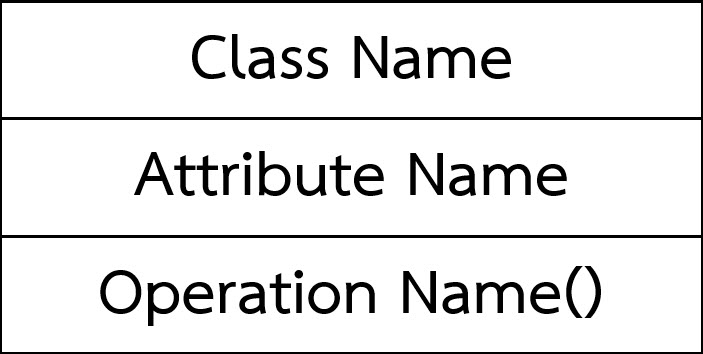
\includegraphics[width=0.3\textwidth]{Figures/table/class/11}}
			& \setstretch{1.5} {คลาส สัญลักษณ์แทนด้วยสี่เหลี่ยมแบ่งเป็น 3 ส่วน 
				ส่วนบน เป็นชื่อของ class ส่วนกลาง เป็นชื่อ Attribute และส่วนล่างเป็น Operation Name หรือ Method ใช้สำหรับเขียนฟังก์ชันในการทำงานของคลาสนั้น ๆ
				ชนิดของ Visibility ของ Method และ Attribute
				แบ่งเป็น 3 ชนิด ได้แก่
				\begin{enumerate}
					\item Public แทนสัญลักษณ์ด้วยเครื่องหมายบวก (+)
					\item Private แทนสัญลักษณ์ด้วยเครื่องหมายลบ (-)
					\item Protected แทนสัญลักษณ์ด้วยเครื่องหมายชาร์ป (#)
				\end{enumerate}
			} \\ \hline
			\raisebox{-\totalheight}{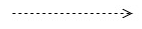
\includegraphics[width=0.3\textwidth]{Figures/table/class/1}}
			& \setstretch{1.5} {Dependency Relationship หมายความว่า คลาสที่อยู่ฝั่งต้นลูกศรสามารถเรียกใช้คลาสที่อยู่ฝั่งหัวลูกศร}
			\\ \hline
			\raisebox{-\totalheight}{
\includegraphics[width=0.35\textwidth]{Figures/3/Class/aggre}}
			& \setstretch{1.5} {Composition Relationship เป็นความสัมพันธ์ระหว่างออบเจ็กต์หรือคลาสแบบขึ้นต่อกันและมีความเกี่ยวข้องกันเสมอ} \\ \hline
			\raisebox{-\totalheight}{
\includegraphics[width=0.3\textwidth]{Figures/3/Class/implement}}
			& \setstretch{1.5} {Realization Relationship เป็นความสัมพันธ์ระหว่าง Object หรือ Class ในลักษณะของการสืบทอดคุณสมบัติจาก Class หนึ่ง (Super class) ไปยังอีก Class หนึ่ง (Subclass)} \\ \hline
			\raisebox{-\totalheight}{
\includegraphics[width=50,height=50]{Figures/table/class/connector}}
			& \setstretch{1.5} {Connector เป็นสัญลักษณ์แทนด้วยรูปห้าเหลี่ยมและมีชื่ออยู่ตรงกลาง จะสร้างสัญลักษณ์นี้ไว้เมื่อต้องการเชื่อมต่อคลาสที่อยู่คนละหน้า} \\ \hline
		\end{tabular}
	\end{table}
	\end{center}

\newpage
  %IMAGE of class
	Class Diagram แสดงความสัมพันธ์ในรูปแบบต่างๆ ระหว่างคลาสของแอปพลิเคชันสูงวัยมายเฟรนด์ อธิบายได้ตามภาพที่ \ref{Fig:MainActivity20C} ดังต่อไปนี้

\begin{sidewaysfigure}
	\begin{figure}[H]
		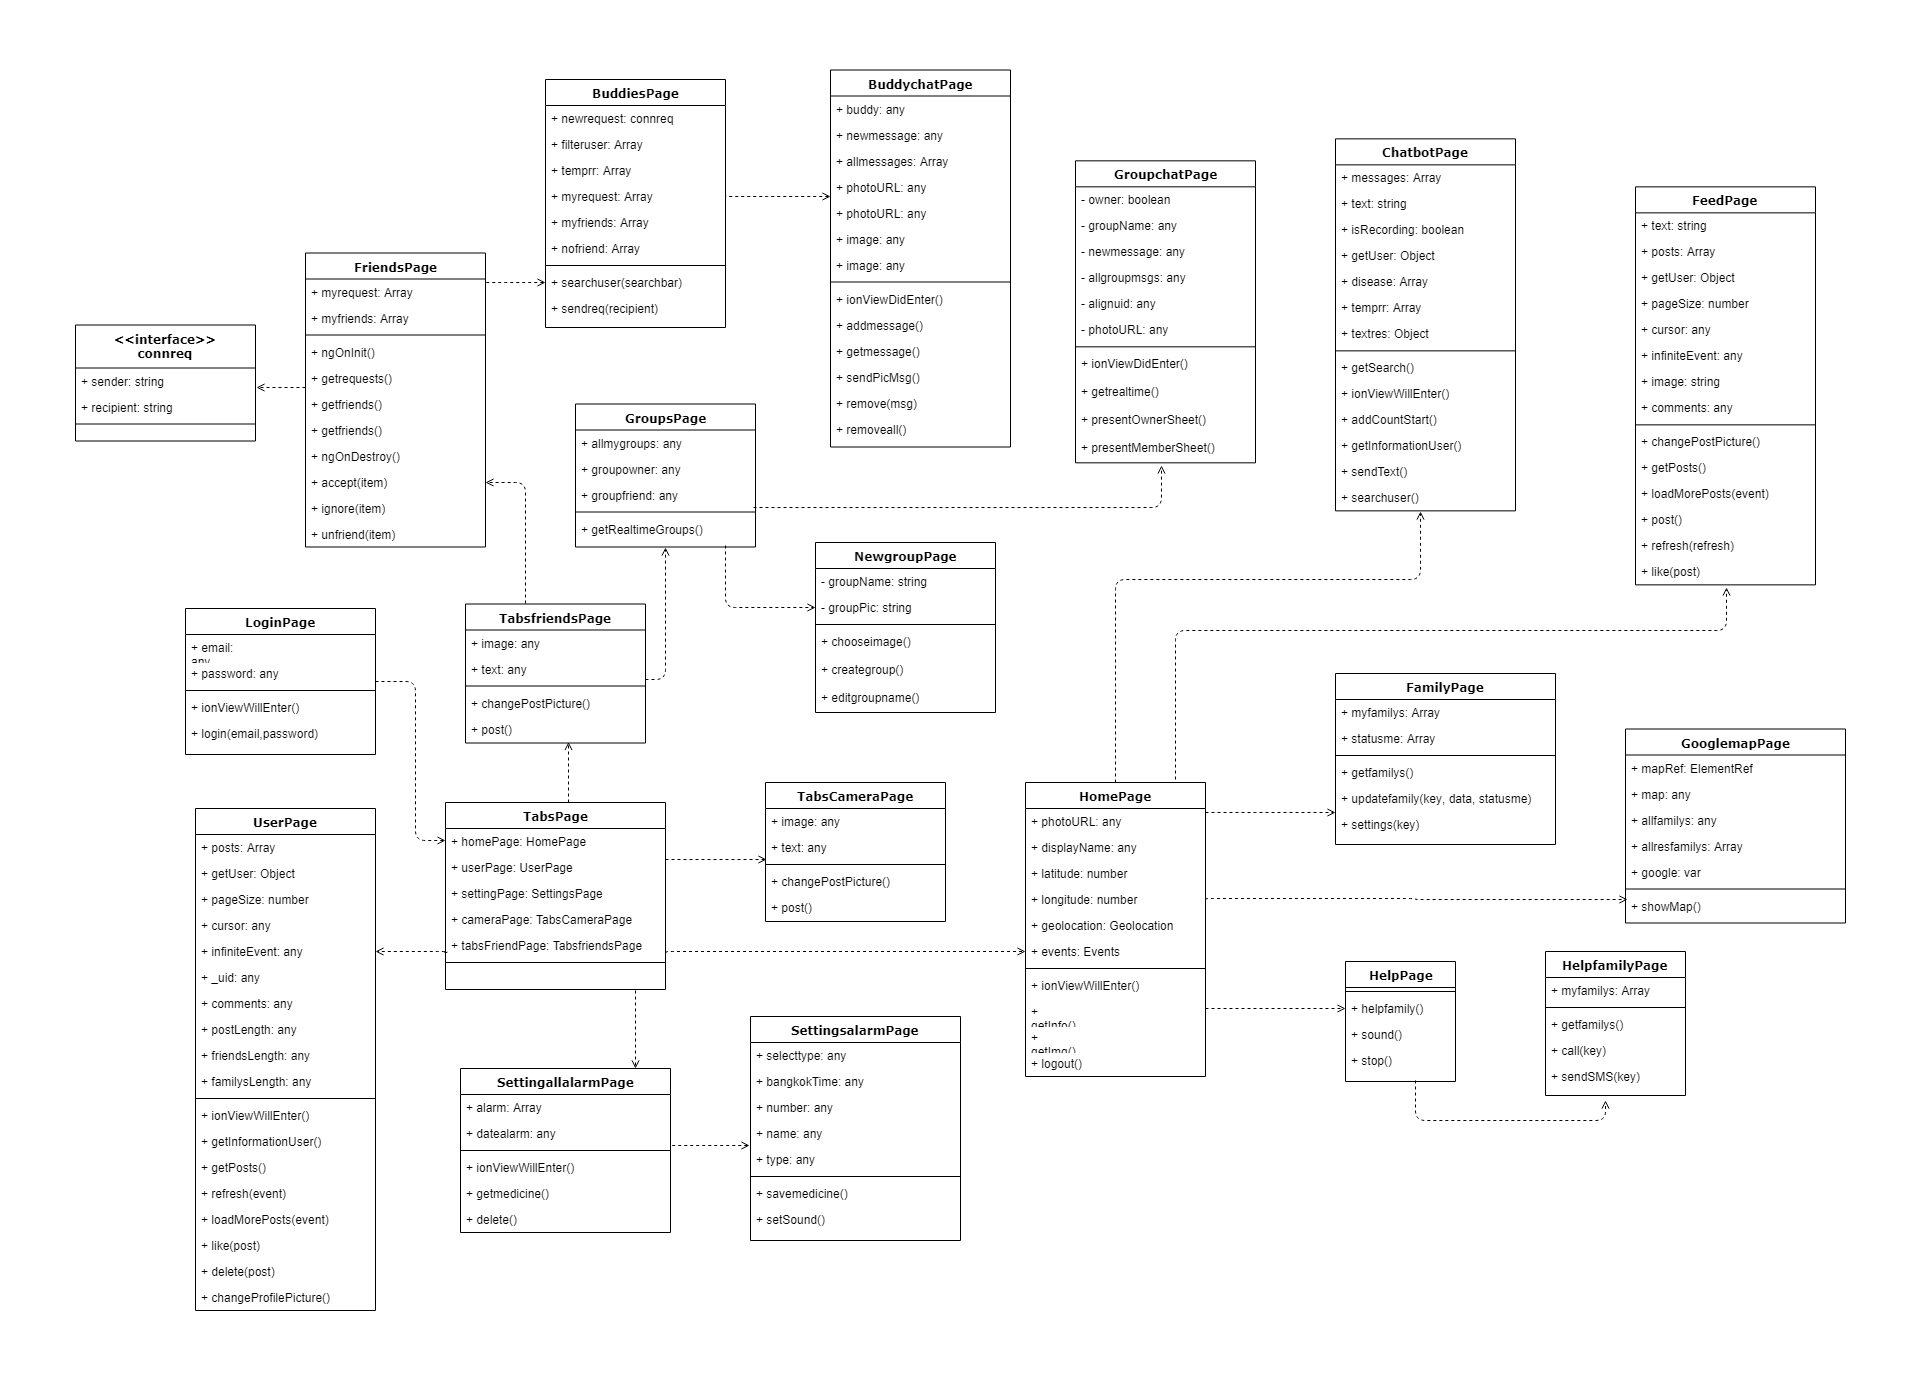
\includegraphics[width=1.0\columnwidth]{Figures/3/Class/classdiagrams}
		\caption{Class Diagram ของแอปพลิเคชันสูงวัยมายเฟรนด์}
		\label{Fig:classdiagram}
	\end{figure}
\end{sidewaysfigure}


	% TABLE of class
\newpage	
	จากรูปภาพที่ \ref{Fig:classdiagram} สามารถอธิบายแผนภาพ Class Diagram ได้ดังนี้
	\begin{table}[H]
		\centering
		\caption{อธิบาย Class Diagram ของแอปพลิเคชันสูงวัยมายเฟรนด์}
		\label{tab:class}
		\begin{tabular}{|c|p{10cm}|}
			\hline
			\textbf{Class Diagram} & \multicolumn{1}{c|}{\textbf{คำอธิบาย}} \\ \hline
			\raisebox{-\totalheight}{LoginPage}
			& \setstretch{1.5} {คลาส LoginPage เป็นคลาสที่ใช้เพื่อให้ผู้ใช้ที่ได้ลงทะเบียนกับระบบไว้แล้วเข้าระบบเพื่อใช้งานแอปพลิเคชัน } \\ \hline
			\raisebox{-\totalheight}{TabsPage}
			& \setstretch{1.5} {คลาส TabsPage เป็นคลาสที่ถูกเรียกเพื่อจัดการ Tabs} \\ \hline
			\raisebox{-\totalheight}{TabsfriendsPage}
			& \setstretch{1.5} {คลาส TabsfriendsPage เป็นคลาสที่ใช้แสดงสมาชิกกลุ่ม คำร้องขอเพิ่มเพื่อนและเพื่อน} \\ \hline
			\raisebox{-\totalheight}{FriendsPage}
			& \setstretch{1.5} {คลาส FriendsPage เป็นคลาสที่ใช้แสดงคำร้องขอเพื่อนและเพื่อน} \\ \hline
			\raisebox{-\totalheight}{connreq}
			& \setstretch{1.5} {คลาส connreq เป็นคลาสที่ใช้เก็บข้อมูลคำร้องขอเพื่อน} \\ \hline
			\raisebox{-\totalheight}{BuddiesPage}
			& \setstretch{1.5} {คลาส BuddiesPage เป็นคลาสที่ใช้สำหรับการเพิ่มเพื่อน} \\ \hline
			\raisebox{-\totalheight}{BuddychatPage}
			& \setstretch{1.5} {คลาส BuddychatPage เป็นคลาสที่ใช้สำหรับแชทกับเพื่อน} \\ \hline
			\raisebox{-\totalheight}{BuddychatPage}
			& \setstretch{1.5} {คลาส BuddychatPage เป็นคลาสที่ใช้สำหรับแชทกับเพื่อน} \\ \hline
			\raisebox{-\totalheight}{GroupsPage}
			& \setstretch{1.5} {คลาส GroupsPage เป็นคลาสที่แสดงกลุ่มของฉันและกลุ่มที่เป็นสมาชิก} \\ \hline
			\raisebox{-\totalheight}{NewgroupPage}
			& \setstretch{1.5} {คลาส NewgroupPage เป็นคลาสที่ใช้สร้างกลุ่ม} \\ \hline
			\raisebox{-\totalheight}{GroupchatPage}
			& \setstretch{1.5} {คลาส GroupchatPage เป็นคลาสสำหรับการแชทกลุ่ม} \\ \hline
			\raisebox{-\totalheight}{SettingallalarmPage}
			& \setstretch{1.5} {คลาส SettingallalarmPage เป็นคลาสที่แสดงการแจ้งเตือนการทานยาทั้งหมด} \\ \hline
			\raisebox{-\totalheight}{SettingsalarmPage}
			& \setstretch{1.5} {คลาส SettingsalarmPage เป็นคลาสที่ใช้บันทึกการแจ้งเตือนการทานยา} \\ \hline
			\raisebox{-\totalheight}{TabsCameraPage}
			& \setstretch{1.5} {คลาส TabsCameraPage เป็นคลาสที่ใช้สำหรับสร้างโพสท์} \\ \hline
			\raisebox{-\totalheight}{HomePage}
			& \setstretch{1.5} {คลาส HomePage เป็นคลาสสำหรับการแสดงหน้าเมนูหลักของแอปพลิเคชัน} \\ \hline
			\raisebox{-\totalheight}{ChatbotPage}
			& \setstretch{1.5} {คลาส ChatbotPage เป็นคลาสที่ใช้สำหรับพูดคุยกับแชทบอท} \\ \hline
			\raisebox{-\totalheight}{FeedPage}
			& \setstretch{1.5} {คลาส FeedPage เป็นคลาสที่แสดงโพสท์ทั้งหมด} \\ \hline
	\end{tabular}
\end{table}

\begin{table}[H]
	\centering
	\caption{อธิบาย Class Diagram ของแอปพลิเคชันสูงวัยมายเฟรนด์}
	\label{tab:class}
	\begin{tabular}{|c|p{10cm}|}
		\hline
		\textbf{Class Diagram} & \multicolumn{1}{c|}{\textbf{คำอธิบาย}} \\ \hline
		\raisebox{-\totalheight}{FamilyPage}
		& \setstretch{1.5} {คลาส FamilyPage เป็นคลาสที่แสดงสมาชิกในครอบครัว} \\ \hline
		\raisebox{-\totalheight}{GooglemapPage}
		& \setstretch{1.5} {คลาส GooglemapPage เป็นคลาสที่แสดงตำแหน่งของสมาชิกในครอบครัวด้วย Google Map} \\ \hline
		\raisebox{-\totalheight}{HelpPage}
		& \setstretch{1.5} {คลาส HelpPage เป็นคลาสที่แสดงรูปภาพขอความช่วยเหลือ 2 แบบ คือ แบบติดต่อครอบครัว และแบบส่งเสียงฉุกเฉิน} \\ \hline
		\raisebox{-\totalheight}{HelpfamilyPage}
		& \setstretch{1.5} {คลาส HelpfamilyPage เป็นคลาสแสดงสมาชิกในครอบครัวเพื่อขอความช่วยเหลือมี 2 แบบได้แก่ โทร และส่งข้อความ} \\ \hline
\end{tabular}
\end{table}

\newpage

%  สิ้นสุด Class Diagram

%  เริ่มต้น Squence Diagram

\section{ซีเควนไดอะแกรม (Sequence Diagram)}
	Sequence Diagram เป็น Diagram ที่แสดงขั้นตอนการทำงานของแต่ละ Use Case ระหว่าง Object ต่างๆ ที่ส่งข้อความถึงกันและกัน โดย Sequence Diagram จะช่วยให้มองเห็นการทำงานของภาพรวมของระบบ ส่วนประกอบสัญลักษณ์ที่ใช้ในการเขียน Sequence Diagram 
	แสดงดังตารางที่ \ref{tab:Sequences}
	
	\begin{table}[H]
		\centering
		\caption{สัญลักษณ์ของ Sequence Diagram}
		\label{tab:Sequences}
		\begin{tabular}{|c|p{10cm}|}
		\hline
		\textbf{สัญลักษณ์} & \multicolumn{1}{c|}{\textbf{การใช้งาน}} \\ \hline
		\raisebox{-\totalheight}{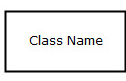
\includegraphics[width=0.17\textwidth]{Figures/table/Sequence/Sequence1}}
		& \setstretch{1.5} {Class แสดงถึงการทำงานของ Use Case ในการส่งหรือรับข้อความ แทนด้วยสัญลักษณ์สี่เหลี่ยมมีชื่อคลาสอยู่ภายใน} \\ \hline
		\raisebox{-\totalheight}{
\includegraphics[height=0.08\textheight]{Figures/table/Sequence/Sequence2}}
		& \setstretch{1.5} {Lifeline หรือเส้นอายุขัย แสดงช่วงเวลาตั้งแต่เริ่มสร้าง object ในคลาสนั้น จนกระทั่ง object นั้นถูกทำลาย สัญลักษณ์แทนด้วยเส้นประ} \\ \hline
		\raisebox{-\totalheight}{
\includegraphics[height=0.08\textheight]{Figures/table/Sequence/Sequence3}}
		& \setstretch{1.5} {Focus of control หรือจุดควบคุม เป็นจุดควบคุมที่ object ใช้ทำการส่งหรือรับข้อความ สัญลักษณ์แทนด้วยสี่เหลี่ยม} \\ \hline
		\raisebox{-\totalheight}{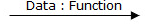
\includegraphics[width=0.3\textwidth]{Figures/table/Sequence/Sequence4}}
		& \setstretch{1.5} {Message คือ ข้อความที่รับส่งระหว่าง Object สัญลักษณ์แทนด้วยลูกศรและประกอบด้วย 2 ส่วน คือ ข้อมูล (Data) และฟังก์ชัน (Function)} \\ \hline
		\raisebox{-\totalheight}{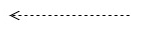
\includegraphics[width=0.3\textwidth]{Figures/table/Sequence/Sequence5}}
		& \setstretch{1.5} {Return Message เป็นข้อมูลที่ส่งกลับหลังจากทำงานเสร็จ} \\ \hline
		\raisebox{-\totalheight}{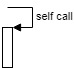
\includegraphics[height=0.08\textheight]{Figures/3/selfcall}}
		& \setstretch{1.5} {Self call เป็นการเรียกฟังชันก์การทำงานภายในตัวเอง} \\ \hline
		\raisebox{-\totalheight}{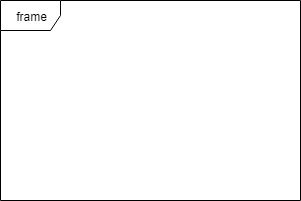
\includegraphics[height=0.1\textheight,width=0.3\textwidth]{Figures/3/frame}}
		& \setstretch{1.5} {สร้างกรอบการทำงานของโปรแกรม เพื่อให้รู้ขอบเขตของการทำงานเช่น ลูป(loop)} \\ \hline
		\end{tabular}
	\end{table}
%
Sequence Diagram ที่ใช้อธิบายการทำงานของแอปพลิเคชันสูงวัยมายเฟรนด์ มีรายละเอียดดังต่อไปนี้
\begin{sidewaysfigure}
	\begin{figure}[H]
		\centering
		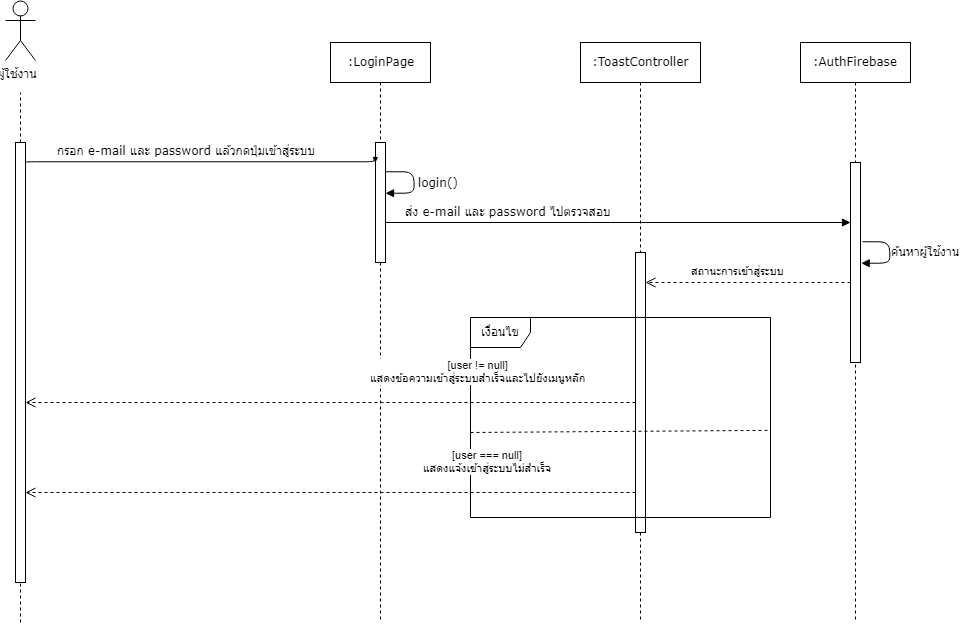
\includegraphics[width=0.8\columnwidth]
		{Figures/3/Sequence/login}
		\caption{Sequence Diagram การเข้าสู่ระบบ}
		\label{Fig:Sequence-login}
	\end{figure}
\end{sidewaysfigure}
	จากภาพที่ \ref{Fig:Sequence-login} สามารถอธิบายแผนภาพ Sequence Diagram การเข้าสู่ระบบ ได้ดังนี้
	เมื่อผู้ใช้กรอก e-mail และ password แล้วกดปุ่มเข้าสู่ระบบ จากนั้นระบบจะเรียกฟังก์ชัน login() เพื่อส่งข้อมูลไปตรวจที่ AuthFibase ที่เป็นบริการ
	ของ Firebase ในการเข้าสู่ระบบด้วยอีเมลล์ จากนั้นจะส่งข้อมูลกลับมายัง ToastController เพื่อเช็คข้อมูลว่ามีหรือไม่ ถ้ามีข้อมูลจะแสดงข้อความว่า 
	เข้าสู่ระบบสำเร็จและไปยังหน้าหลัก ถ้าไม่สำเร็จระบบจะแสดงข้อความว่า กรุณากรอกชื่อผู้ใช้หรือรหัสผ่านให้ถูกต้อง
	\newpage	

	\begin{sidewaysfigure}
	\begin{figure}[H]
		\centering
		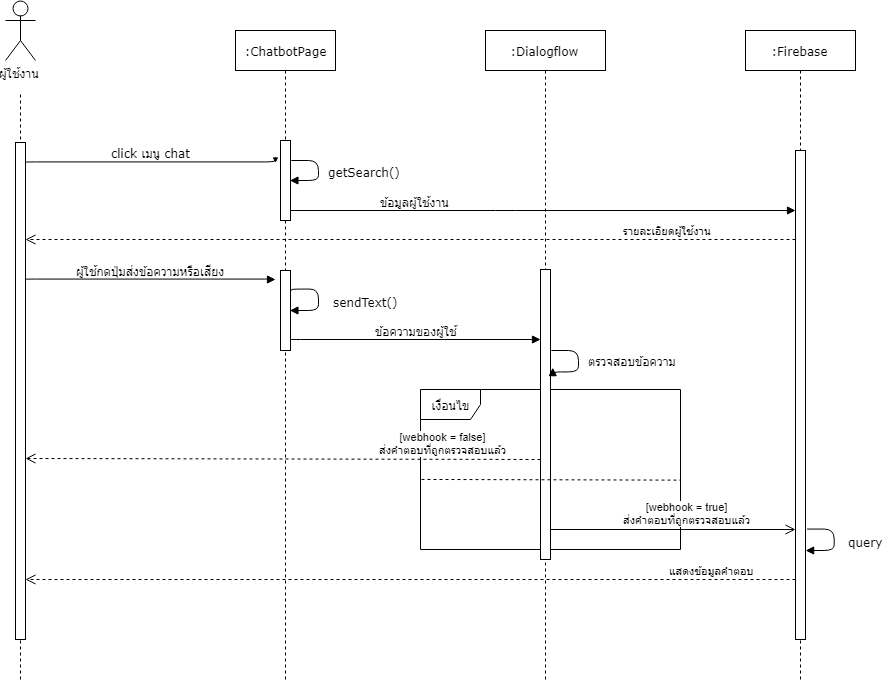
\includegraphics[width=0.8\columnwidth]
		{Figures/3/Sequence/chatbot}
		\caption{Sequence Diagram คุยกับแชทบอท}
		\label{Fig:Sequence-chatbot}
	\end{figure}
\end{sidewaysfigure}
	\newpage
	จากภาพที่ \ref{Fig:Sequence-chatbot} สามารถอธิบายแผนภาพ Sequence Diagram คุยกับแชทบอท ได้ดังนี้ 
	เมื่อผู้ใช้เปิดใช้งานหน้าปู่สนทนากับแชทบอท ระบบจะทำการบันทึกข้อมูลการค้นหาข้อมูลเป็น 0 ในไฟล์เบส เพื่อใช้สำหรับเช็คการค้นหาที่ถูกค้นหามากที่สุด
	แล้วไฟล์เบสก็จะส่งข้อมูลกลับคืนมาหาผู้ใช้ ถ้าผู้ใช้ส่งในรูปแบบข้อความหรือเสียงถ้าหากเป็นเสียงจะแปลงเป็นข้อความก่อน หลังจากนั้นข้อความจะถูกส่งไป Dialogflow 
	เพื่อประมวลผลใน Intent เพื่อหาคำตอบถ้าหาก Intent นั้นไม่ได้ใช้งาน webhook Dialogflow จะส่งข้อความกลับคืนหาผู้ใช้ตามคำตอบที่ได้ตั้งค่าไว้ ถ้าหาก Intent นั้น
	ได้เปิด webhook จะส่งข้อความไปตรวจสอใน Fullfillment เพื่อตรวจสอบคำสำคัญในข้อความ หลังจากนั้นจะถูกส่งไปเช็คใน Firebase แล้วส่ง
	คำตอบกลับมายังผู้ใช้
	\newpage	


	\begin{figure}[H]
		\centering
		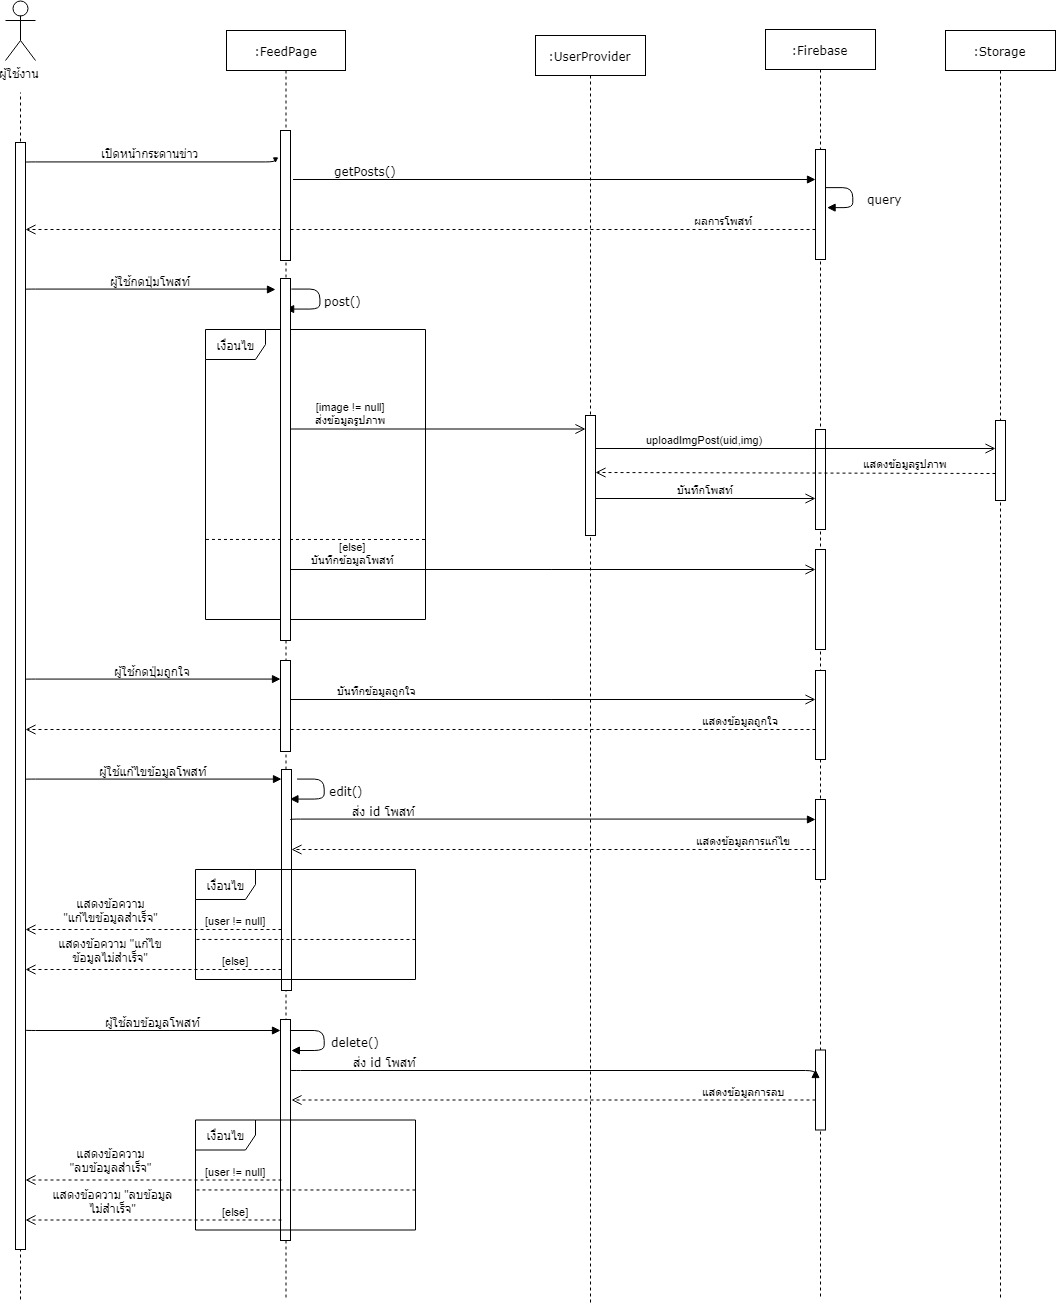
\includegraphics[width=1.0\columnwidth]
		{Figures/3/Sequence/feed}
		\caption{Sequence Diagram การแสดงหน้ากระดานข่าว}
		\label{Fig:Sequence-feed}
	\end{figure}
	\newpage
	จากภาพที่ \ref{Fig:Sequence-doc} สามารถอธิบายแผนภาพ Sequence Diagram การแสดงหน้ากระดานข่าว ได้ดังนี้ 
	\begin{itemize}
	\item เมื่อผู้ใช้งานเข้ามายังหน้ากระดานข่าว ระบบจะดึงข้อมูลมาจากไฟล์เบสเพื่อแสดงโพสท์ทั้งหมด เมื่อผู้ใช้กดปุ่มโพสท์ระบบจะเรียกฟังก์ชัน post() 
	ระบบจะตรวจสอบว่าข้อมูลที่เราต้องการโพสท์มีการเพิ่มรูปหรือไม่ ถ้ามีรูประบบส่งที่อยู่รูปไปทำงานฟังก์ชัน uploadImgPost(uid,img) 
	เพื่อเก็บข้อมูลลงใน Firebas Storage หลังจากนั้นจะบันทึกโพสท์ที่เราสร้างไว้ใน Firebase ถ้าโพสท์ไม่มีรูปภาพจะบันทึกข้อมูลไว้ใน Firebase ทันที 
	\item เมื่อผู้ใช้กดปุ่มถูกใจ ระบบจะส่งข้อมูลไอดีของผู้ที่กดส่งไปเก็บไว้ยังฐานข้อมูล Firebase แล้วจึงส่ง Response กลับมาหาผู้ใช้
	\item เมื่อผู้ใช้กดเลือกเมนูแก้ไขโพสท์แล้วกดปุ่มบันทึกข้อมูล ระบบจะทำการเรียกใช้ฟังก์ชัน edit() เพื่อส่ง id ไปเช็คข้อมูลใน Firebase แล้วจึงแก้ไขข้อมูล หากมี Response กลับคืนมาจะแสดงข้อความบันทึกข้อมูลสำเร็จ แต่ถ้าไม่มี Response กลับคืนมาจะแสดงข้อความว่าบันทึกข้อมูลไม่สำเร็จ
	\item เมื่อผู้ใช้กดเลือกเมนูลบโพสท์แล้วกดปุ่มยืนยัน ระบบจะทำการเรียกใช้ฟังก์ชัน delete() เพื่อส่ง id ไปเช็คข้อมูลใน Firebase แล้วจึงลบข้อมูล หากมี Response กลับคืนมาจะแสดงลบข้อมูลสำเร็จ แต่ถ้าไม่มี Response กลับคืนมาจะแสดงข้อความว่าลบข้อมูลไม่สำเร็จ
	\end{itemize}
	\newpage	

\begin{sidewaysfigure}
	\begin{figure}[H]
		\centering
		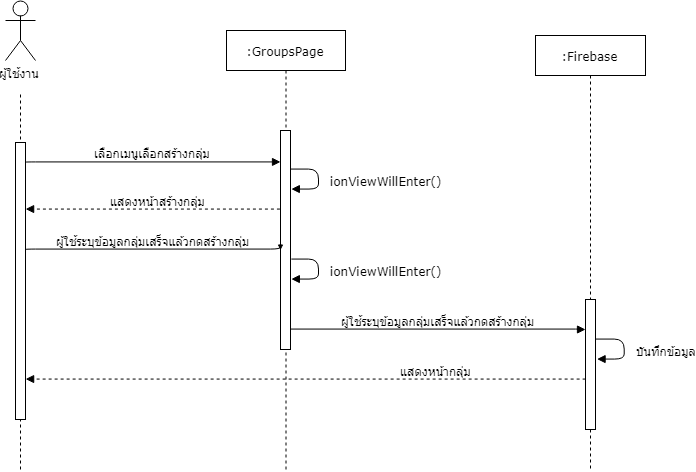
\includegraphics[width=0.8\columnwidth]
		{Figures/3/Sequence/addgroup}
		\caption{Sequence Diagram ของการเพิ่มกลุ่ม}
		\label{Fig:Sequence-addgroup}
	\end{figure}
\end{sidewaysfigure}
	จากภาพที่ \ref{Fig:Sequence-addgroup} สามารถอธิบายแผนภาพ Sequence Diagram ของการเพิ่มกลุ่ม ได้ดังนี้ เมื่อผู้ใช้
	กดปุ่มเพิ่มกลุ่มระบบจะเรียกฟังก์ชัน ionViewWillEnter() เพื่อแสดงหน้าเพิ่มกลุ่ม ต่อมาผู้ใช้กรอกข้อมูลเสร็จแล้วกดสร้างกลุ่ม 
	จากนั้นระบบจะเรียกฟังก์ชัน creategroup() ในคลาส NewGroupsPage เพื่อบันทึกข้อมูลลงใน Firebase เมื่อเพิ่มฐานข้อมูลเสร็จเรียบร้อยแล้ว 
	ระบบจะแสดงหน้ากลุ่ม
	\newpage	


	\begin{figure}[H]
		\centering
		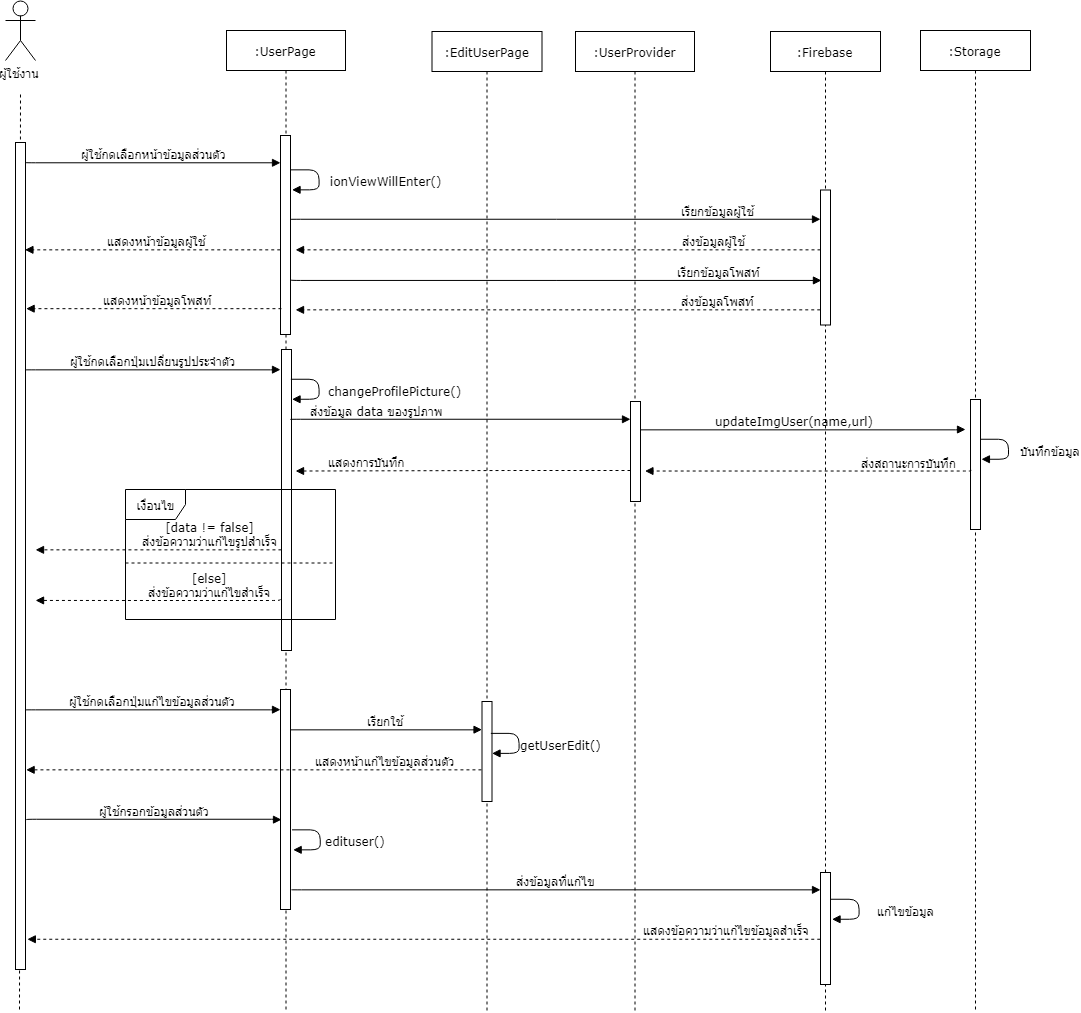
\includegraphics[width=1.0\columnwidth]
		{Figures/3/Sequence/edituser}
		\caption{Sequence Diagram ของการจัดการข้อมูลส่วนตัว}
		\label{Fig:Sequence-edituser}
	\end{figure}
	\newpage
	จากภาพที่ \ref{Fig:Sequence-edituser} สามารถอธิบายแผนภาพ Sequence Diagram ของการจัดการข้อมูลส่วนตัว ได้ดังนี้ 
	\begin{itemize}
		\item เมื่อผู้ใช้กดเลือกหน้าข้อมูลส่วนตัว ระบบจะเรียกฟังก์ชัน ionViewWillEnter() เพื่อเรียกข้อมูลผู้ใช้และโพสท์จากฐานข้อมูลมาแสดงหน้าข้อมูลส่วนตัว
		\item เมื่อผู้ใช้กดเลือกปุ่มเปลี่ยนรูปประจำตัว ระบบจะเรียกฟังก์ชัน changeProfilePicture() เพื่อให้ผู้ใช้เลือกรูปแบบการแก้ไขรูปภาพจาก camera plugin เพื่อใช้งานกล้องและแกลลอรี่ 
		หลังจากนั้นจะส่งข้อมูล url ไปยัง Firebase storage เพื่อทำการเพิ่มหรือแก้ไขข้อมูล แล้วส่งสถานะกลับมายังผู้ใช้งาน ถ้าหากสามารถเปลี่ยนได้จะส่งข้อความว่า แก้ไขรูปสำเร็จ 
		แต่ถ้าไม่สามารถแก้ไขรูปได้จะส่งข้อความว่า แก้ไขไม่สำเร็จ 
		\item เมื่อผู้ใช้เลือกปุ่มแก้ไขข้อมูลส่วนตัว ระบบจะเรียกฟังก์ชัน getUserEdit() ในคลาส EditUserPage จากนั้นจะแสดงหน้าแก้ไขข้อมูลส่วนตัว เมื่อผู้ใช้กรอกข้อมูลส่วนตัวเรียบร้อยแล้ว จะเรียกฟังก์ชัน edituser() 
		จากนั้นจะส่งข้อมูลที่ถูกแก้ไขไปฐานข้อมูล ฐานข้อมูลตรวจสอบและอัพเดทข้อมูลที่ถูกแก้ไข จากนั้นฐานข้อมูลจะส่งข้อความกลับมาว่า แก้ไขข้อมูลสำเร็จแล้ว
		\end{itemize}
\newpage	

	\begin{figure}[H]
		\centering
		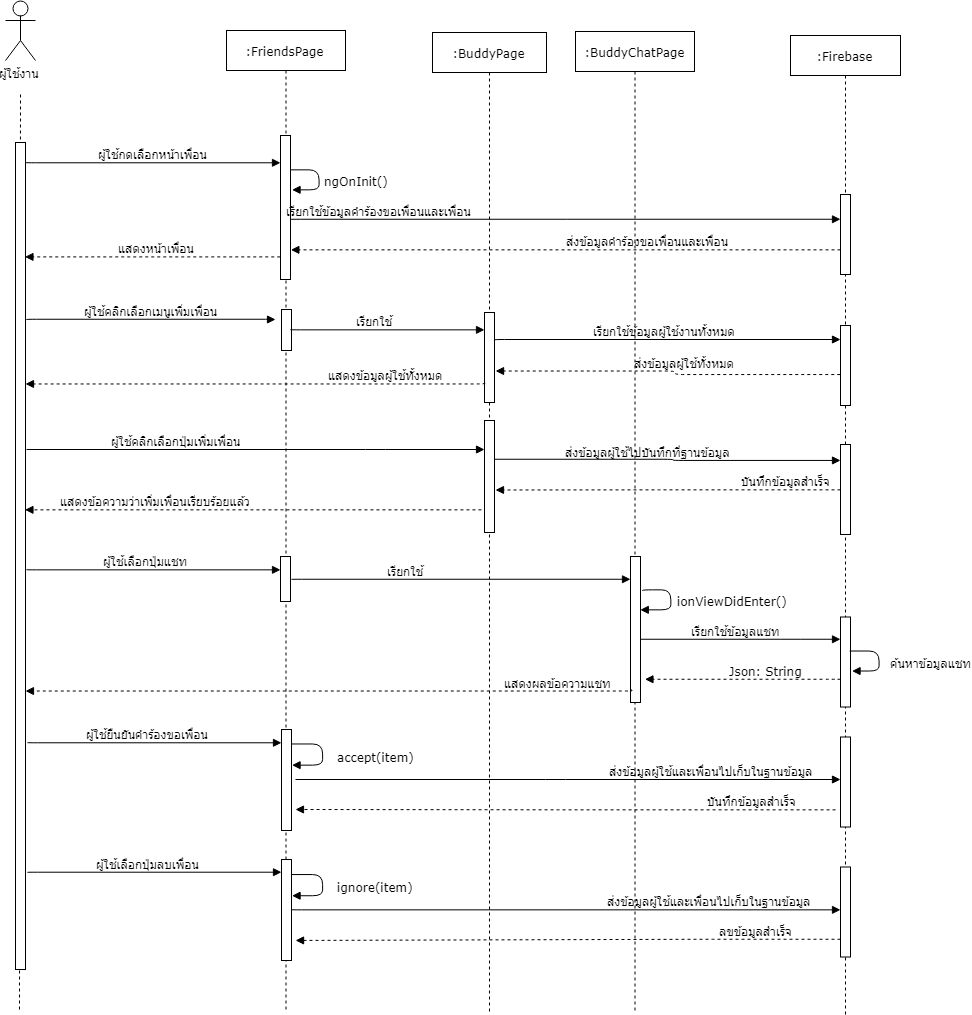
\includegraphics[width=1.0\columnwidth]
		{Figures/3/Sequence/friend}
		\caption{Sequence Diagram ของการจัดการเพื่อน}
		\label{Fig:Sequence-friend}
	\end{figure}
	\newpage
	จากภาพที่ \ref{Fig:Sequence-friend} สามารถอธิบายแผนภาพ Sequence Diagram ของการจัดการเพื่อน ได้ดังนี้ 
	\begin{itemize}
		\item เมื่อผู้ใช้เลือกเมนูเพื่อน ระบบจะเรียกฟังก์ชัน ngOnit() ในคลาส FriendsPage จะไป get ข้อมูลจาก Firebase เพื่อมาแสดง
		\item เมื่อผู้ใช้คลิกเลือกเมนูเพิ่มเพื่อน จะเรียกใช้คลาส BuddyPage จากนั้นระบบจะไป get ข้อมูลคำร้องขอเพื่อนและเพื่อนจาก Firebase มาแสดงในคลาส 
		\item เมื่อผู้ใช้เลือกปุ่มเพิ่มเพื่อนในคลาส BuddyPage จะส่งข้อมูล id ของผู้และ id ของเพื่อนไปเก็บไว้ในฐานข้อมูล หลังจากนั้นฐานข้อมูลจะส่งผลการบันทึกข้อมูลสำเร็จมาที่คลาส แล้วระบบจะส่งข้อความว่าเพิ่มเพื่อนเรียบร้อยแล้วมายังผู้ใช้
		\item ผู้ใช้เลือกปุ่มแชทในคลาส FriendsPage ระบบจะเรียกใช้ฟังก์ชัน ionViewDidEnter() ในคลาส BuddychatPage เพื่อไปเรียกข้อมูลการแชททั้งหมดจากฐานข้อมูล จากนั้นฐานข้อมูลจะส่งค่า Json กลับคืนมายังคลาส BuddychatPage แล้วจึงแสดงข้อความแชทให้ผู้ใช้
		\item เมื่อผู้ใช้ยืนยันคำร้องขอเพื่อน ระบบจะเรียกฟังก์ชัน accept(item) จะรับข้อมูล Json ของเพื่อนเพื่อดึง id ไปเก็บไว้ในฐานข้อมูล จากนั้นฐานข้อมูลจะส่งผลการบันทึกข้อความคืนมายังคลาส
		\item เมื่อผู้ใช้เลือกปุ่มลบเพื่อน ระบบจะทำการเรียกใช้ฟังก์ชัน ignore(item) จากนั้นจะส่งค่า id ของเพื่อนไปเช็คในฐานข้อมูล แล้วลบข้อมูลผู้ใช้นั้น แล้วจึงส่งผลการลบข้อมูลกลับมายังคลาส
		\end{itemize}
\newpage	 


\begin{figure}[H]
	\centering
	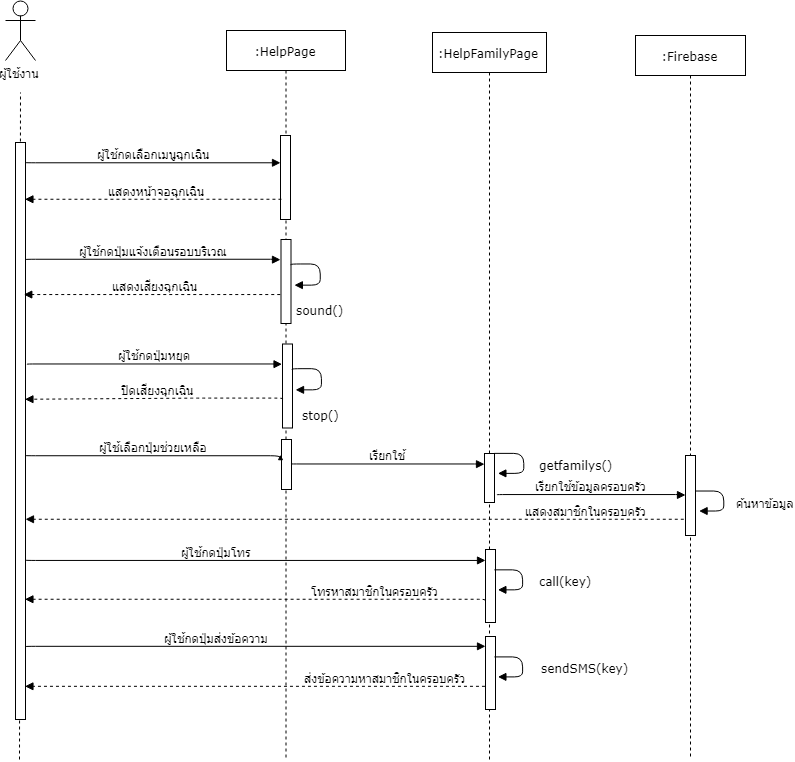
\includegraphics[width=1.0\columnwidth]
	{Figures/3/Sequence/danger}
	\caption{Sequence Diagram ของฉุกเฉิน}
	\label{Fig:Sequence-danger}
\end{figure}

\newpage
จากภาพที่ \ref{Fig:Sequence-danger} สามารถอธิบายแผนภาพ Sequence Diagram ของฉุกเฉิน ได้ดังนี้ 
ผู้ใช้กดเลือกเมนฉุกเฉิน ระบบจะเรียกฟังก์ชัน ionViewWillEnter() ในคลาสแสดงหน้าฉุกเฉิน เมื่อผู้ใช้กดปุ่มแจ้งเตือนรอบบริเวณ ระบบจะเรียกฟังก์ชัน sound() เพื่อใช้งาน NativeAudio Plugin ที่ใช้สำหรับแสดงเสียงแล้วแสดงเสียงแก่ผู้ใช้งาน 
เมื่อผู้ใช้คลิกที่ปุ่มหยุด ระบบจะหยุดเสียงที่ผู้ใช้ได้กดปุ่มแจ้งเตือนรอบบริเวณก่อนหน้านี้ เมื่อผู้ใช้เลือกปุ่มช่วยเหลือ จะเรียกใช้คลาส HelpFamilyPage จากนั้น Contructor จะเรียกข้อมูลสมาชิกครอบครัวในฐานข้อมูลมาแสดง 
ถ้าผู้ใช้กดปุ่มโทร ระบบจะเรียกฟังก์ชัน call(key) จากนั้นจะ get เบอร์มือถือของเพื่อนเพื่อใช้ CallNumber Plugin สำหรับโทร เมื่อผู้ใช้กดปุ่มส่งข้อความ ระบบจะเรียกฟังก์ชัน sendSMS(key) ที่อยู่ภายในคลาส HelpFamilyPage และเรียกใช้ SocialSharing Plugin ในการส่ง SMS ที่
มีข้อความว่า "ช่วยด้วย !!! นี่ (ชื่อผู้ใช้) เอง ตอนนี้มีปัญหาช่วยติดต่อกลับที่ (เบอร์มือถือผู้ใช้) ด้วยนะ ด่วน ๆ"
\newpage

	
% \section{โครงสร้างฐานข้อมูลไฟร์เบส(Firebase Database Stucture)}
% Firebase Database นั้นเป็น Database แบบ NoSQL และเป็น JSON database ที่มีโครงสร้างที่เป็น Key และ Value จัดเก็บข้อมูลในลักษณะโหนด หากต้องการเรียกงานจะเรียกใช้โดย
% การท่องไปยังโหนดที่ต้องการ ส่วนประกอบสัญลักษณ์ที่ใช้ในการเขียนโครงสร้างฐานข้อมูลแบบ Firebase
% แสดงดังตารางที่ \ref{tab:DB}

% \begin{table}[H]
% 	\centering
% 	\caption{สัญลักษณ์ของโครงสร้างฐานข้อมูลแบบ Firebase}
% 	\label{tab:DB}
% 	\begin{tabular}{| c	| p{10cm} |}
% 		\hline
% 		\textbf{สัญลักษณ์} & \multicolumn{1}{c|}{\textbf{คำอธิบาย}} \\ \hline
% 		\raisebox{-\totalheight}{
\includegraphics[width=0.1\textwidth]{Figures/3/DB/dbroot}}
% 		& \setstretch{1.5} {Database เป็นการเรียกชื่อแทนโหนด(Node)บนสุดที่ใช้ในการเก็บข้อมูล} \\ \hline
% 		\raisebox{-\totalheight}{
\includegraphics[width=0.1\textwidth]{Figures/3/DB/dbcollection}}
% 		& \setstretch{1.5} {Collection เป็นการเรียกชื่อแทนของการเก็บหลาย ๆ เอกสารไว้ด้วยกัน} \\ \hline
% 		\raisebox{-\totalheight}{
\includegraphics[width=0.1\textwidth]{Figures/3/DB/dbdoc}}
% 		& \setstretch{1.5} {Document เป็นการเรียกชื่อแทนหน่วยการเก็บของข้อมูลใน Cloud Firestore ภายในจะประกอบไปด้วย ชื่อของ Document  ชื่อของคีย์ (key) และ ค่าข้อมูล (value) โดยชื่อของ Document ห้ามซ้ำกัน ซึ่งใน Cloud Firestore สามารถระบุประเภทของข้อมูลได้ 9 ประเภทได้แก่ boolean, number, string, geo point, timestamp, array, object, reference และ null} \\ \hline
% 	\end{tabular}
% \end{table}
% 	\begin{figure}[H]
% 	\centering
% 	\includegraphics[width=0.7\columnwidth]
% 	{Figures/3/DB/DB1}
% 	\caption{โครงสร้างฐานข้อมูลแบบ Firebase}
% 	\label{Fig:DB1}
% 	\end{figure}

% 	\begin{figure}[H]
% 	\centering
% 	\includegraphics[width=0.9\columnwidth]
% 	{Figures/3/DB/DB2}
% 	\caption{โครงสร้างฐานข้อมูลแบบ Firebase(ต่อ)}
% 	\label{Fig:DB2}
% \end{figure}
% 	\begin{figure}[H]
% 	\centering
% 	\includegraphics[width=0.55\columnwidth]
% 	{Figures/3/DB/DB3}
% 	\caption{โครงสร้างฐานข้อมูลแบบ Firebase(ต่อ)}
% 	\label{Fig:DB3}
% \end{figure}
% 	\begin{figure}[H]
% 	\centering
% 	\includegraphics[width=0.7\columnwidth]
% 	{Figures/3/DB/DB4}
% 	\caption{โครงสร้างฐานข้อมูลแบบ Firebase(ต่อ)}
% 	\label{Fig:DB4}
% \end{figure}

% \newpage
% จากรูที่ \ref{Fig:DB1}-\ref{Fig:DB4} สามารถอธิบายโครงสร้างของข้อมูลได้ดังนี้
% \begin{figure}[H]
% \centering
% \includegraphics[width=0.5\columnwidth]
% {Figures/3/DB/nodePost}
% \caption{โหนดเก็บข้อมูลประกาศ}
% \label{Fig:DB4}
% \end{figure}
% \begin{table}[H]
% 	\centering
% 	\caption{อธิบายโหนดที่ใช้เก็บข้อมูลประกาศ}
% 	\label{my-label1}
% 	\begin{tabular}{|c|p{10cm}|}
% 		\hline
% 		\multicolumn{1}{|c|}{\textbf{Key}} & \multicolumn{1}{c|}{\textbf{คำอธิบาย}} \\ \hline
% 		Posts & โหนดสำหรับเก็บข้อมูลประกาศทั้งหมด \\ \hline
% 		Post &  สำหรับเก็บข้อมูลแต่ละประกาศ \\ \hline
% 		title & สำหรับเก็บชื่อหัวข้อประกาศ \\ \hline
% 		description & สำหรับเก็บรายละเอียดประกาศ  \\ \hline
% 		collection & สำหรับเก็บประเภทของประกาศได้แก่ สาธารณะและเฉพาะบุคคล \\ \hline
% 		fileURL & สำหรับเก็บ url ของเอกสารแนบประกาศ \\ \hline
% 		id & สำหรับเก็บรหัสของประกาศ \\ \hline
% 		time & สำหรับเก็บเวลาที่ประกาศ \\ \hline
% 	\end{tabular}
% \end{table}

% \newpage
% \begin{figure}[H]
% 	\centering
% 	\includegraphics[width=0.5\columnwidth]
% 	{Figures/3/DB/nodeDoc}
% 	\caption{โหนดเก็บข้อมูลเอกสารที่เกี่ยวข้อง}
% 	\label{Fig:DB4}
% \end{figure}
% \begin{table}[H]
% 	\centering
% 	\caption{อธิบายโหนดที่ใช้เก็บข้อมูลเอกสารที่เกี่ยวข้อง}
% 	\label{my-label1}
% 	\begin{tabular}{|c|p{10cm}|}
% 		\hline
% 		\multicolumn{1}{|c|}{\textbf{Key}} & \multicolumn{1}{c|}{\textbf{คำอธิบาย}} \\ \hline
% 		Docs & โหนดสำหรับเก็บข้อมูลของเอกสารที่เกี่ยวข้องทั้งหมด \\ \hline
% 		Doc &  สำหรับเก็บข้อมูลเอกสารแต่ละฉบับ \\ \hline
% 		title & สำหรับเก็บชื่อหัวเรื่องของเอกสาร \\ \hline
% 		description & สำหรับเก็บรายละเอียดของเอกสาร \\ \hline
% 		fileType & สำหรับนามสกุลไฟล์เอกสาร เช่น .pdf .png เป็นต้น \\ \hline
% 		fileURL & สำหรับเก็บ url ของเอกสาร\\ \hline
% 		time & สำหรับเก็บเวลาที่ถูกอัพโหลดเข้าสู่ระบบโดยเจ้าหน้าที่\\ \hline
% 	\end{tabular}
% \end{table}

% \newpage
% \begin{figure}[H]
% 	\centering
% 	\includegraphics[width=0.4\columnwidth]
% 	{Figures/3/DB/nodeChat}
% 	\caption{โหนดเก็บข้อมูลประวัติการสนทนา}
% 	\label{Fig:DB4}
% \end{figure}
% \begin{table}[H]
% 	\centering
% 	\caption{อธิบายโหนดที่ใช้เก็บข้อมูลประวัติการสนทนา}
% 	\label{my-label1}
% 	\begin{tabular}{|c|p{10cm}|}
% 		\hline
% 		\multicolumn{1}{|c|}{\textbf{Key}} & \multicolumn{1}{c|}{\textbf{คำอธิบาย}} \\ \hline
% 		Chats & โหนดสำหรับเก็บข้อมูลประวัติการสนทนาทั้งหมด \\ \hline
% 		User\_id &  สำหรับเก็บประวัติการสนทนาของผู้ใช้แต่ละคน \\ \hline
% 		Messages & สำหรับเก็บประวัติการสนทนาทั้งหมดของผู้ใช้ \\ \hline
% 		Message & สำหรับเก็บข้อมูลของแต่ละข้อความ \\ \hline
% 		message & สำหรับเก็บข้อความ \\ \hline
% 		name & สำหรับเก็บชื่อของผู้ส่งข้อความ\\ \hline
% 		photo & สำหรับเก็บ url รูปภาพของผู้ส่งข้อความ\\ \hline
% 		senderId & สำหรับเก็บรหัสของผู้ส่งข้อความ\\ \hline
% 		time & สำหรับเก็บเวลาที่ข้อความถูกส่ง\\ \hline
% 	\end{tabular}
% \end{table}

% \newpage
% \begin{figure}[H]
% 	\centering
% 	\includegraphics[width=0.5\columnwidth]
% 	{Figures/3/DB/nodeEvent}
% 	\caption{โหนดเก็บข้อมูลกำหนดการ}
% 	\label{Fig:DB4}
% \end{figure}
% \begin{table}[H]
% 	\centering
% 	\caption{อธิบายโหนดที่ใช้เก็บข้อมูลกำหนดการ}
% 	\label{my-label1}
% 	\begin{tabular}{|c|p{10cm}|}
% 		\hline
% 		\multicolumn{1}{|c|}{\textbf{Key}} & \multicolumn{1}{c|}{\textbf{คำอธิบาย}} \\ \hline
% 		Events & โหนดสำหรับเก็บข้อมูลของกำหนดการทั้งหมด \\ \hline
% 		Event & สำหรับเก็บข้อมูลของแต่ละกำหนดการ \\ \hline
% 		title & สำหรับเก็บชื่อหัวข้อของกำหนดการ \\ \hline
% 		description & สำหรับเก็บรายละเอียดของกำหนดการ\\ \hline
% 		time & สำหรับเก็บเวลาของกำหนดการ\\ \hline
% 	\end{tabular}
% \end{table}

% \newpage
% \begin{figure}[H]
% 	\centering
% 	\includegraphics[width=0.4\columnwidth]
% 	{Figures/3/DB/nodeReq}
% 	\caption{โหนดเก็บข้อมูลการยื่นสำเนาเอกสารเพื่อตรวจสอบของนักศึกษา}
% 	\label{Fig:DB4}
% \end{figure}
% \begin{table}[H]
% 	\centering
% 	\caption{อธิบายโหนดที่ใช้เก็บข้อมูลการยื่นสำเนาเอกสารเพื่อตรวจสอบของนักศึกษา}
% 	\label{my-label1}
% 	\begin{tabular}{|c|p{10cm}|}
% 		\hline
% 		\multicolumn{1}{|c|}{\textbf{Key}} & \multicolumn{1}{c|}{\textbf{คำอธิบาย}} \\ \hline
% 		RusetSubmitDocs & โหนดสำหรับเก็บข้อมูลการยื่นสำเนาเอกสารเพื่อตรวจสอบของนักศึกษาทั้งหมด \\ \hline
% 		User\_id & สำหรับเก็บข้อมูลของแต่ละสำเนาเอกสารของนักศึกษาแต่ละคน \\ \hline
% 		doc2 & สำหรับเก็บ url ของภาพถ่ายสำเนาเอกสารฉบับที่ 1\\ \hline
% 		doc2 & สำหรับเก็บ url ของภาพถ่ายสำเนาเอกสารฉบับที่ 2\\ \hline
% 		status & สำหรับเก็บผลการตรวจสอบของเจ้าหน้าที่ \\ \hline
% 		time & สำหรับเก็บเวลาที่สำเนาเอกสารถูกเพิ่มเข้าสู่ระบบ \\ \hline
% 	\end{tabular}
% \end{table}

% \newpage
% \begin{figure}[H]
% 	\centering
% 	\includegraphics[width=0.35\columnwidth]
% 	{Figures/3/DB/nodeUser}
% 	\caption{โหนดเก็บข้อมูลของนักศึกษา}
% 	\label{Fig:DB4}
% \end{figure}
% \begin{table}[H]
% 	\centering
% 	\caption{อธิบายโหนดที่ใช้เก็บข้อมูลของนักศึกษา}
% 	\label{my-label1}
% 	\begin{tabular}{|c|p{10cm}|}
% 		\hline
% 		\multicolumn{1}{|c|}{\textbf{Key}} & \multicolumn{1}{c|}{\textbf{คำอธิบาย}} \\ \hline
% 		Users & โหนดสำหรับเก็บข้อมูลของนักศึกษา \\ \hline
% 		User\_id & สำหรับเก็บข้อมูลของนักศึกษาแต่ละคน \\ \hline
% 		depart & สำหรับเก็บภาควิชาของนักศึกษา\\ \hline
% 		major & สำหรับเก็บสาขาของนักศึกษา\\ \hline
% 		sid & สำหรับเก็บรหัสประจำตัวนักศึกษา \\ \hline
% 		name & สำหรับเก็บชื่อของนักศึกษา \\ \hline
% 		year & สำหรับเก็บชั้นปีของนักศึกษา \\ \hline
% 		lastChat & สำหรับเก็บเวลาที่สนทนากับเจ้าหน้าที่ล่าสุด \\ \hline
% 		photoUrl & สำหรับเก็บ url รูปภาพโปรไฟล์ (Profile) \\ \hline
% 	\end{tabular}
% \end{table}

% \newpage
% \begin{figure}[H]
% 	\centering
% 	\includegraphics[width=0.5\columnwidth]
% 	{Figures/3/DB/nodeQueue}
% 	\caption{โหนดเก็บข้อมูลการจองคิวของนักศึกษา}
% 	\label{Fig:DB4}
% \end{figure}
% \begin{table}[H]
% 	\centering
% 	\caption{อธิบายโหนดที่ใช้เก็บข้อมูลการจองคิวของนักศึกษา}
% 	\label{my-label1}
% 	\begin{tabular}{|c|p{10cm}|}
% 		\hline
% 		\multicolumn{1}{|c|}{\textbf{Key}} & \multicolumn{1}{c|}{\textbf{คำอธิบาย}} \\ \hline
% 		Queue & โหนดสำหรับเก็บข้อมูลการจองคิวของนักศึกษาทั้งหมด \\ \hline
% 		q\_id &  สำหรับเก็บข้อมูลของการจองคิวแต่ละครั้งที่เปิดจองคิว \\ \hline
% 		Date &  สำหรับเก็บวันที่สำหรับส่งเอกสาร\\ \hline
% 		Time &  สำหรับเก็บรายชื่อของนักศึกษาที่ทำการจองคิวในส่งเอกสารเวลานั้น ๆ\\ \hline
% 		User\_id & สำหรับเก็บรหัสของนักศึกษา \\ \hline
% 		title & สำหรับเก็บชื่อหัวเรื่องกำหนดการการจองคิว \\ \hline
% 		studentPerHr & สำหรับเก็บจำนวนนักศึกษาต่อชั่วโมง \\ \hline
% 	\end{tabular}
% \end{table}

% \newpagedr
% \begin{figure}[H]
% 	\centering
% 	\includegraphics[width=0.4\columnwidth]
% 	{Figures/3/DB/nodeFaq}
% 	\caption{โหนดเก็บข้อมูลคำถามที่พบบ่อย}
% 	\label{Fig:DB4}
% \end{figure}
% \begin{table}[H]
% 	\centering
% 	\caption{อธิบายโหนดที่ใช้เก็บข้อมูลคำถามที่พบบ่อย}
% 	\label{my-label1}
% 	\begin{tabular}{|c|p{10cm}|}
% 		\hline
% 		\multicolumn{1}{|c|}{\textbf{Key}} & \multicolumn{1}{c|}{\textbf{คำอธิบาย}} \\ \hline
% 		Queue & โหนดสำหรับเก็บข้อมูลคำถามที่พบบ่อยทั้งหมด \\ \hline
% 		Faq\_id & สำหรับเก็บข้อมูลคำถามที่พบบ่อยแต่ละรายการ \\ \hline
% 		title & สำหรับเก็บคำถาม \\ \hline
% 		description & สำหรับเก็บคำตอบ \\ \hline
% 	\end{tabular}
% \end{table}
